%&preformat-disser
\RequirePackage[l2tabu,orthodox]{nag} % Раскомментировав, можно в логе получать рекомендации относительно правильного использования пакетов и предупреждения об устаревших и нерекомендуемых пакетах
% Формат А4, 14pt (ГОСТ Р 7.0.11-2011, 5.3.6)
\documentclass[a4paper,14pt,oneside,openany]{memoir}

%%%%%%%%%%%%%%%%%%%%%%%%%%%%%%%%%%%%%%%%%%%%%%%%%%%%%%
%%%% Файл упрощённых настроек шаблона диссертации %%%%
%%%%%%%%%%%%%%%%%%%%%%%%%%%%%%%%%%%%%%%%%%%%%%%%%%%%%%

%%% Инициализирование переменных, не трогать!  %%%
\newcounter{intvl}
\newcounter{otstup}
\newcounter{contnumeq}
\newcounter{contnumfig}
\newcounter{contnumtab}
\newcounter{pgnum}
\newcounter{chapstyle}
\newcounter{headingdelim}
\newcounter{headingalign}
\newcounter{headingsize}
%%%%%%%%%%%%%%%%%%%%%%%%%%%%%%%%%%%%%%%%%%%%%%%%%%%%%%

%%% Область упрощённого управления оформлением %%%

%% Интервал между заголовками и между заголовком и текстом %%
% Заголовки отделяют от текста сверху и снизу
% тремя интервалами (ГОСТ Р 7.0.11-2011, 5.3.5)
\setcounter{intvl}{3}               % Коэффициент кратности к размеру шрифта

%% Отступы у заголовков в тексте %%
\setcounter{otstup}{0}              % 0 --- без отступа; 1 --- абзацный отступ

%% Нумерация формул, таблиц и рисунков %%
% Нумерация формул
\setcounter{contnumeq}{0}   % 0 --- пораздельно (во введении подряд,
                            %       без номера раздела);
                            % 1 --- сквозная нумерация по всей диссертации
% Нумерация рисунков
\setcounter{contnumfig}{0}  % 0 --- пораздельно (во введении подряд,
                            %       без номера раздела);
                            % 1 --- сквозная нумерация по всей диссертации
% Нумерация таблиц
\setcounter{contnumtab}{1}  % 0 --- пораздельно (во введении подряд,
                            %       без номера раздела);
                            % 1 --- сквозная нумерация по всей диссертации

%% Оглавление %%
\setcounter{pgnum}{1}       % 0 --- номера страниц никак не обозначены;
                            % 1 --- Стр. над номерами страниц (дважды
                            %       компилировать после изменения настройки)
\settocdepth{subsection}    % до какого уровня подразделов выносить в оглавление
\setsecnumdepth{subsection} % до какого уровня нумеровать подразделы


%% Текст и форматирование заголовков %%
\setcounter{chapstyle}{1}     % 0 --- разделы только под номером;
                              % 1 --- разделы с названием "Глава" перед номером
\setcounter{headingdelim}{1}  % 0 --- номер отделен пропуском в 1em или \quad;
                              % 1 --- номера разделов и приложений отделены
                              %       точкой с пробелом, подразделы пропуском
                              %       без точки;
                              % 2 --- номера разделов, подразделов и приложений
                              %       отделены точкой с пробелом.

%% Выравнивание заголовков в тексте %%
\setcounter{headingalign}{0}  % 0 --- по центру;
                              % 1 --- по левому краю

%% Размеры заголовков в тексте %%
\setcounter{headingsize}{0}   % 0 --- по ГОСТ, все всегда 14 пт;
                              % 1 --- пропорционально изменяющийся размер
                              %       в зависимости от базового шрифта

%% Подпись таблиц %%

% Смещение строк подписи после первой строки
\newcommand{\tabindent}{0cm}

% Тип форматирования заголовка таблицы:
% plain --- название и текст в одной строке
% split --- название и текст в разных строках
\newcommand{\tabformat}{plain}

%%% Настройки форматирования таблицы `plain`

% Выравнивание по центру подписи, состоящей из одной строки:
% true  --- выравнивать
% false --- не выравнивать
\newcommand{\tabsinglecenter}{false}

% Выравнивание подписи таблиц:
% justified   --- выравнивать как обычный текст («по ширине»)
% centering   --- выравнивать по центру
% centerlast  --- выравнивать по центру только последнюю строку
% centerfirst --- выравнивать по центру только первую строку (не рекомендуется)
% raggedleft  --- выравнивать по правому краю
% raggedright --- выравнивать по левому краю
\newcommand{\tabjust}{justified}

% Разделитель записи «Таблица #» и названия таблицы
\newcommand{\tablabelsep}{~\cyrdash\ }

%%% Настройки форматирования таблицы `split`

% Положение названия таблицы:
% \centering   --- выравнивать по центру
% \raggedleft  --- выравнивать по правому краю
% \raggedright --- выравнивать по левому краю
\newcommand{\splitformatlabel}{\raggedleft}

% Положение текста подписи:
% \centering   --- выравнивать по центру
% \raggedleft  --- выравнивать по правому краю
% \raggedright --- выравнивать по левому краю
\newcommand{\splitformattext}{\raggedright}

%% Подпись рисунков %%
%Разделитель записи «Рисунок #» и названия рисунка
\newcommand{\figlabelsep}{~\cyrdash\ }  % (ГОСТ 2.105, 4.3.1)
                                        % "--- здесь не работает

%%% Цвета гиперссылок %%%
% Latex color definitions: http://latexcolor.com/
\definecolor{linkcolor}{rgb}{0,0,0}
\definecolor{citecolor}{rgb}{0,0,0}
\definecolor{urlcolor}{rgb}{0,0,1}
%\definecolor{linkcolor}{rgb}{0,0,0} %black
%\definecolor{citecolor}{rgb}{0,0,0} %black
%\definecolor{urlcolor}{rgb}{0,0,0} %black
            % общие настройки шаблона
%%% Проверка используемого TeX-движка %%%
\newif\ifxetexorluatex   % определяем новый условный оператор (http://tex.stackexchange.com/a/47579)
\ifxetex
    \xetexorluatextrue
\else
    \ifluatex
        \xetexorluatextrue
    \else
        \xetexorluatexfalse
    \fi
\fi

\newif\ifsynopsis           % Условие, проверяющее, что документ --- автореферат

\usepackage{etoolbox}[2015/08/02]   % Для продвинутой проверки разных условий
\providebool{presentation}

\usepackage{comment}    % Позволяет убирать блоки текста (добавляет
                        % окружение comment и команду \excludecomment)

%%% Поля и разметка страницы %%%
\usepackage{pdflscape}  % Для включения альбомных страниц
\usepackage{geometry}   % Для последующего задания полей

%%% Математические пакеты %%%
\usepackage{amsthm,amsmath,amscd}   % Математические дополнения от AMS
\usepackage{amsfonts,amssymb}       % Математические дополнения от AMS
\usepackage{mathtools}              % Добавляет окружение multlined
\usepackage{xfrac}                  % Красивые дроби
\usepackage[
    locale = DE,
    list-separator       = {;\,},
    list-final-separator = {;\,},
    list-pair-separator  = {;\,},
    list-units           = single,
    range-units          = single,
    range-phrase={\text{\ensuremath{-}}},
    % quotient-mode        = fraction, % красивые дроби могут не соответствовать ГОСТ
    fraction-function    = \sfrac,
    separate-uncertainty,
    ]{siunitx}[=v2]                 % Размерности SI
\sisetup{inter-unit-product = \ensuremath{{}\cdot{}}}

% Кириллица в нумерации subequations
% Для правильной работы требуется выполнение сразу после загрузки пакетов
\patchcmd{\subequations}{\def\theequation{\theparentequation\alph{equation}}}
{\def\theequation{\theparentequation\asbuk{equation}}}
{\typeout{subequations patched}}{\typeout{subequations not patched}}

%%%% Установки для размера шрифта 14 pt %%%%
%% Формирование переменных и констант для сравнения (один раз для всех подключаемых файлов)%%
%% должно располагаться до вызова пакета fontspec или polyglossia, потому что они сбивают его работу
\newlength{\curtextsize}
\newlength{\bigtextsize}
\setlength{\bigtextsize}{13.9pt}

\makeatletter
%\show\f@size    % неплохо для отслеживания, но вызывает стопорение процесса,
                 % если документ компилируется без команды  -interaction=nonstopmode
\setlength{\curtextsize}{\f@size pt}
\makeatother

%%% Кодировки и шрифты %%%
\ifxetexorluatex
    \ifpresentation
        \providecommand*\autodot{} % quick fix for polyglossia 1.50
    \fi
    \PassOptionsToPackage{no-math}{fontspec}    % https://tex.stackexchange.com/a/26295/104425
    \usepackage{polyglossia}[2014/05/21]        % Поддержка многоязычности
                                        % (fontspec подгружается автоматически)
\else
   %%% Решение проблемы копирования текста в буфер кракозябрами
    \ifnumequal{\value{usealtfont}}{0}{}{
        \input glyphtounicode.tex
        \input glyphtounicode-cmr.tex %from pdfx package
        \pdfgentounicode=1
    }
    \usepackage{cmap}   % Улучшенный поиск русских слов в полученном pdf-файле
    \ifnumequal{\value{usealtfont}}{2}{}{
        \defaulthyphenchar=127  % Если стоит до fontenc, то переносы
                                % не впишутся в выделяемый текст при
                                % копировании его в буфер обмена
    }
    \usepackage{textcomp}
    \usepackage[T1,T2A]{fontenc}                    % Поддержка русских букв
    \ifnumequal{\value{usealtfont}}{1}{% Используется pscyr, при наличии
        \IfFileExists{pscyr.sty}{\usepackage{pscyr}}{}  % Подключение pscyr
    }{}
    \usepackage[utf8]{inputenc}[2014/04/30]         % Кодировка utf8
    \usepackage[english, russian]{babel}[2014/03/24]% Языки: русский, английский
    \makeatletter\AtBeginDocument{\let\@elt\relax}\makeatother % babel 3.40 fix
    \ifnumequal{\value{usealtfont}}{2}{
        % http://dxdy.ru/post1238763.html#p1238763
        \usepackage[scaled=0.914]{XCharter}[2017/12/19] % Подключение русифицированных шрифтов XCharter
        \usepackage[charter, vvarbb, scaled=1.048]{newtxmath}[2017/12/14]
        \ifpresentation
        \else
            \setDisplayskipStretch{-0.078}
        \fi
    }{}
\fi

%%% Оформление абзацев %%%
\ifpresentation
\else
    \indentafterchapter     % Красная строка после заголовков типа chapter
    \usepackage{indentfirst}
\fi

%%% Цвета %%%
\ifpresentation
\else
    \usepackage[dvipsnames, table, hyperref]{xcolor} % Совместимо с tikz
\fi

%%% Таблицы %%%
\usepackage{longtable,ltcaption} % Длинные таблицы
\usepackage{multirow,makecell}   % Улучшенное форматирование таблиц
\usepackage{tabu, tabulary}      % таблицы с автоматически подбирающейся
                                 % шириной столбцов (tabu обязательно
                                 % до hyperref вызывать)
\makeatletter
%https://github.com/tabu-issues-for-future-maintainer/tabu/issues/26
\@ifpackagelater{longtable}{2020/02/07}{
\def\tabuendlongtrial{%
    \LT@echunk  \global\setbox\LT@gbox \hbox{\unhbox\LT@gbox}\kern\wd\LT@gbox
                \LT@get@widths
}%
}{}
\makeatother

\usepackage{threeparttable}      % автоматический подгон ширины подписи таблицы

%%% Общее форматирование
\usepackage{soulutf8}% Поддержка переносоустойчивых подчёркиваний и зачёркиваний
\usepackage{icomma}  % Запятая в десятичных дробях

%%% Оптимизация расстановки переносов и длины последней строки абзаца
\IfFileExists{impnattypo.sty}{% проверка установленности пакета impnattypo
    \ifluatex
        \ifnumequal{\value{draft}}{1}{% Черновик
            \usepackage[hyphenation, lastparline, nosingleletter, homeoarchy,
            rivers, draft]{impnattypo}
        }{% Чистовик
            \usepackage[hyphenation, lastparline, nosingleletter]{impnattypo}
        }
    \else
        \usepackage[hyphenation, lastparline]{impnattypo}
    \fi
}{}

%% Векторная графика

\usepackage{tikz}                   % Продвинутый пакет векторной графики
\usetikzlibrary{chains}             % Для примера tikz рисунка
\usetikzlibrary{shapes.geometric}   % Для примера tikz рисунка
\usetikzlibrary{shapes.symbols}     % Для примера tikz рисунка
\usetikzlibrary{arrows}             % Для примера tikz рисунка

%%% Гиперссылки %%%
\ifxetexorluatex
    \let\CYRDZE\relax
\fi
\usepackage{hyperref}[2012/11/06]

%%% Изображения %%%
\usepackage{graphicx}[2014/04/25]   % Подключаем пакет работы с графикой
\usepackage{caption}                % Подписи рисунков и таблиц
\usepackage{subcaption}             % Подписи подрисунков и подтаблиц
\usepackage{pdfpages}               % Добавление внешних pdf файлов

%%% Счётчики %%%
\usepackage{aliascnt}
\usepackage[figure,table]{totalcount}   % Счётчик рисунков и таблиц
\usepackage{totcount}   % Пакет создания счётчиков на основе последнего номера
                        % подсчитываемого элемента (может требовать дважды
                        % компилировать документ)
\usepackage{totpages}   % Счётчик страниц, совместимый с hyperref (ссылается
                        % на номер последней страницы). Желательно ставить
                        % последним пакетом в преамбуле

%%% Продвинутое управление групповыми ссылками (пока только формулами) %%%
\ifpresentation
\else
    \usepackage[russian]{cleveref} % cleveref имеет сложности со считыванием
    % языка из babel. Такое решение русификации вывода выбрано вместо
    % определения в documentclass из опасности что-то лишнее передать во все
    % остальные пакеты, включая библиографию.

    % Добавление возможности использования пробелов в \labelcref
    % https://tex.stackexchange.com/a/340502/104425
    \usepackage{kvsetkeys}
    \makeatletter
    \let\org@@cref\@cref
    \renewcommand*{\@cref}[2]{%
        \edef\process@me{%
            \noexpand\org@@cref{#1}{\zap@space#2 \@empty}%
        }\process@me
    }
    \makeatother
\fi

\usepackage{placeins} % для \FloatBarrier

\ifnumequal{\value{draft}}{1}{% Черновик
    \usepackage[firstpage]{draftwatermark}
    \SetWatermarkText{DRAFT}
    \SetWatermarkFontSize{14pt}
    \SetWatermarkScale{15}
    \SetWatermarkAngle{45}
}{}

%%% Цитата, не приводимая в автореферате:
% возможно, актуальна только для biblatex
%\newcommand{\citeinsynopsis}[1]{\ifsynopsis\else ~\cite{#1} \fi}

% если текущий процесс запущен библиотекой tikz-external, то прекомпиляция должна быть включена
\ifdefined\tikzexternalrealjob
    \setcounter{imgprecompile}{1}
\fi

\ifnumequal{\value{imgprecompile}}{1}{% Только если у нас включена предкомпиляция
    \usetikzlibrary{external}   % подключение возможности предкомпиляции
    \tikzexternalize[prefix=images/cache/,optimize command away=\includepdf] % activate! % здесь можно указать отдельную папку для скомпилированных файлов
    \ifxetex
        \tikzset{external/up to date check={diff}}
    \fi
}{}

         % Пакеты общие для диссертации и автореферата
\synopsisfalse                      % Этот документ --- не автореферат
\input{Dissertation/dispackages}    % Пакеты для диссертации
\input{Dissertation/userpackages}   % Пакеты для специфических пользовательских задач

%%%%%%%%%%%%%%%%%%%%%%%%%%%%%%%%%%%%%%%%%%%%%%%%%%%%%%
%%%% Файл упрощённых настроек шаблона диссертации %%%%
%%%%%%%%%%%%%%%%%%%%%%%%%%%%%%%%%%%%%%%%%%%%%%%%%%%%%%

%%% Инициализирование переменных, не трогать!  %%%
\newcounter{intvl}
\newcounter{otstup}
\newcounter{contnumeq}
\newcounter{contnumfig}
\newcounter{contnumtab}
\newcounter{pgnum}
\newcounter{chapstyle}
\newcounter{headingdelim}
\newcounter{headingalign}
\newcounter{headingsize}
%%%%%%%%%%%%%%%%%%%%%%%%%%%%%%%%%%%%%%%%%%%%%%%%%%%%%%

%%% Область упрощённого управления оформлением %%%

%% Интервал между заголовками и между заголовком и текстом %%
% Заголовки отделяют от текста сверху и снизу
% тремя интервалами (ГОСТ Р 7.0.11-2011, 5.3.5)
\setcounter{intvl}{3}               % Коэффициент кратности к размеру шрифта

%% Отступы у заголовков в тексте %%
\setcounter{otstup}{0}              % 0 --- без отступа; 1 --- абзацный отступ

%% Нумерация формул, таблиц и рисунков %%
% Нумерация формул
\setcounter{contnumeq}{0}   % 0 --- пораздельно (во введении подряд,
                            %       без номера раздела);
                            % 1 --- сквозная нумерация по всей диссертации
% Нумерация рисунков
\setcounter{contnumfig}{0}  % 0 --- пораздельно (во введении подряд,
                            %       без номера раздела);
                            % 1 --- сквозная нумерация по всей диссертации
% Нумерация таблиц
\setcounter{contnumtab}{1}  % 0 --- пораздельно (во введении подряд,
                            %       без номера раздела);
                            % 1 --- сквозная нумерация по всей диссертации

%% Оглавление %%
\setcounter{pgnum}{1}       % 0 --- номера страниц никак не обозначены;
                            % 1 --- Стр. над номерами страниц (дважды
                            %       компилировать после изменения настройки)
\settocdepth{subsection}    % до какого уровня подразделов выносить в оглавление
\setsecnumdepth{subsection} % до какого уровня нумеровать подразделы


%% Текст и форматирование заголовков %%
\setcounter{chapstyle}{1}     % 0 --- разделы только под номером;
                              % 1 --- разделы с названием "Глава" перед номером
\setcounter{headingdelim}{1}  % 0 --- номер отделен пропуском в 1em или \quad;
                              % 1 --- номера разделов и приложений отделены
                              %       точкой с пробелом, подразделы пропуском
                              %       без точки;
                              % 2 --- номера разделов, подразделов и приложений
                              %       отделены точкой с пробелом.

%% Выравнивание заголовков в тексте %%
\setcounter{headingalign}{0}  % 0 --- по центру;
                              % 1 --- по левому краю

%% Размеры заголовков в тексте %%
\setcounter{headingsize}{0}   % 0 --- по ГОСТ, все всегда 14 пт;
                              % 1 --- пропорционально изменяющийся размер
                              %       в зависимости от базового шрифта

%% Подпись таблиц %%

% Смещение строк подписи после первой строки
\newcommand{\tabindent}{0cm}

% Тип форматирования заголовка таблицы:
% plain --- название и текст в одной строке
% split --- название и текст в разных строках
\newcommand{\tabformat}{plain}

%%% Настройки форматирования таблицы `plain`

% Выравнивание по центру подписи, состоящей из одной строки:
% true  --- выравнивать
% false --- не выравнивать
\newcommand{\tabsinglecenter}{false}

% Выравнивание подписи таблиц:
% justified   --- выравнивать как обычный текст («по ширине»)
% centering   --- выравнивать по центру
% centerlast  --- выравнивать по центру только последнюю строку
% centerfirst --- выравнивать по центру только первую строку (не рекомендуется)
% raggedleft  --- выравнивать по правому краю
% raggedright --- выравнивать по левому краю
\newcommand{\tabjust}{justified}

% Разделитель записи «Таблица #» и названия таблицы
\newcommand{\tablabelsep}{~\cyrdash\ }

%%% Настройки форматирования таблицы `split`

% Положение названия таблицы:
% \centering   --- выравнивать по центру
% \raggedleft  --- выравнивать по правому краю
% \raggedright --- выравнивать по левому краю
\newcommand{\splitformatlabel}{\raggedleft}

% Положение текста подписи:
% \centering   --- выравнивать по центру
% \raggedleft  --- выравнивать по правому краю
% \raggedright --- выравнивать по левому краю
\newcommand{\splitformattext}{\raggedright}

%% Подпись рисунков %%
%Разделитель записи «Рисунок #» и названия рисунка
\newcommand{\figlabelsep}{~\cyrdash\ }  % (ГОСТ 2.105, 4.3.1)
                                        % "--- здесь не работает

%%% Цвета гиперссылок %%%
% Latex color definitions: http://latexcolor.com/
\definecolor{linkcolor}{rgb}{0,0,0}
\definecolor{citecolor}{rgb}{0,0,0}
\definecolor{urlcolor}{rgb}{0,0,1}
%\definecolor{linkcolor}{rgb}{0,0,0} %black
%\definecolor{citecolor}{rgb}{0,0,0} %black
%\definecolor{urlcolor}{rgb}{0,0,0} %black
      % Упрощённые настройки шаблона

% Новые переменные, которые могут использоваться во всём проекте
% ГОСТ 7.0.11-2011
% 9.2 Оформление текста автореферата диссертации
% 9.2.1 Общая характеристика работы включает в себя следующие основные структурные
% элементы:
% актуальность темы исследования;
\newcommand{\actualityTXT}{Актуальность темы.}
% степень ее разработанности;
\newcommand{\progressTXT}{Степень разработанности темы.}
% цели и задачи;
\newcommand{\aimTXT}{Целью}
\newcommand{\tasksTXT}{задачи}
% научную новизну;
\newcommand{\noveltyTXT}{Научная новизна:}
% теоретическую и практическую значимость работы;
%\newcommand{\influenceTXT}{Теоретическая и практическая значимость}
% или чаще используют просто
\newcommand{\influenceTXT}{Практическая значимость}
% методологию и методы исследования;
\newcommand{\methodsTXT}{Методология и методы исследования.}
% положения, выносимые на защиту;
\newcommand{\defpositionsTXT}{Результаты, выносимые на~защиту:}
% степень достоверности и апробацию результатов.
\newcommand{\reliabilityTXT}{Достоверность.}
\newcommand{\probationTXT}{Апробация работы.}

\newcommand{\contributionTXT}{Личный вклад.}
\newcommand{\publicationsTXT}{Публикации.}


%%% Заголовки библиографии:

% для автореферата:
\newcommand{\bibtitleauthor}{Публикации автора по теме диссертации}

% для стиля библиографии `\insertbiblioauthorgrouped`
\newcommand{\bibtitleauthorvak}{В изданиях из списка ВАК РФ}
\newcommand{\bibtitleauthorscopus}{В изданиях, входящих в международную базу цитирования Scopus}
\newcommand{\bibtitleauthorwos}{В изданиях, входящих в международную базу цитирования Web of Science}
\newcommand{\bibtitleauthorother}{В прочих изданиях}
\newcommand{\bibtitleauthorconf}{В сборниках трудов конференций}
\newcommand{\bibtitleauthorpatent}{Зарегистрированные патенты}
\newcommand{\bibtitleauthorprogram}{Зарегистрированные программы для ЭВМ}

% для стиля библиографии `\insertbiblioauthorimportant`:
\newcommand{\bibtitleauthorimportant}{Наиболее значимые \protect\MakeLowercase\bibtitleauthor}

% для списка литературы в диссертации и списка чужих работ в автореферате:
\newcommand{\bibtitlefull}{Список литературы} % (ГОСТ Р 7.0.11-2011, 4)
         % Новые переменные, для всего проекта

%%% Основные сведения %%%
\newcommand{\thesisAuthorLastName}{Лисицын}
\newcommand{\thesisAuthorOtherNames}{Сергей Алексеевич}
\newcommand{\thesisAuthorInitials}{С.\,А.}
\newcommand{\thesisAuthor}             % Диссертация, ФИО автора
{%
    \texorpdfstring{% \texorpdfstring takes two arguments and uses the first for (La)TeX and the second for pdf
        \thesisAuthorLastName~\thesisAuthorOtherNames% так будет отображаться на титульном листе или в тексте, где будет использоваться переменная
    }{%
        \thesisAuthorLastName, \thesisAuthorOtherNames% эта запись для свойств pdf-файла. В таком виде, если pdf будет обработан программами для сбора библиографических сведений, будет правильно представлена фамилия.
    }
}
\newcommand{\thesisAuthorShort}        % Диссертация, ФИО автора инициалами
{\thesisAuthorInitials~\thesisAuthorLastName}
%\newcommand{\thesisUdk}                % Диссертация, УДК
%{\fixme{xxx.xxx}}
\newcommand{\thesisTitle}              % Диссертация, название
{Исследование и оптимизация применения трасс исполнения приложения для статической бинарной трансляции под RISC архитектуры}
\newcommand{\thesisSpecialtyNumber}    % Диссертация, специальность, номер
{05.13.11}
\newcommand{\thesisSpecialtyTitle}     % Диссертация, специальность, название (название взято с сайта ВАК для примера)
{Математическое и программное обеспечение вычислительных машин, комплексов и компьютерных сетей}
%% \newcommand{\thesisSpecialtyTwoNumber} % Диссертация, вторая специальность, номер
%% {\fixme{XX.XX.XX}}
%% \newcommand{\thesisSpecialtyTwoTitle}  % Диссертация, вторая специальность, название
%% {\fixme{Теория и~методика физического воспитания, спортивной тренировки,
%% оздоровительной и~адаптивной физической культуры}}
\newcommand{\thesisDegree}             % Диссертация, ученая степень
{кандидата технических наук}
\newcommand{\thesisDegreeShort}        % Диссертация, ученая степень, краткая запись
{канд. тех. наук}
\newcommand{\thesisCity}               % Диссертация, город написания диссертации
{Москва}
\newcommand{\thesisYear}               % Диссертация, год написания диссертации
{\the\year}
\newcommand{\thesisOrganization}       % Диссертация, организация
{ФЕДЕРАЛЬНОЕ ГОСУДАРСТВЕННОЕ АВТОНОМНОЕ ОБРАЗОВАТЕЛЬНОЕ УЧРЕЖДЕНИЕ ВЫСШЕГО ОБРАЗОВАНИЯ \\

<<Московский физико-технический институт \\ (национальный исследовательский университет)>> \\ (МФТИ, Физтех)}
\newcommand{\thesisOrganizationShort}  % Диссертация, краткое название организации для доклада
{\fixme{НазУчДисРаб}}

\newcommand{\thesisInOrganization}     % Диссертация, организация в предложном падеже: Работа выполнена в ...
{федеральном государственном автономном образовательном учреждении высшего образования <<Московский физико-технический институт (национальный исследовательский университет)>> (МФТИ)}

%% \newcommand{\supervisorDead}{}           % Рисовать рамку вокруг фамилии
\newcommand{\supervisorFio}              % Научный руководитель, ФИО
{Плоткин Арнольд Леонидович}
\newcommand{\supervisorRegalia}          % Научный руководитель, регалии
{д.т.н., профессор}
\newcommand{\supervisorFioShort}         % Научный руководитель, ФИО
{А.\,Л.~Плоткина}
\newcommand{\supervisorRegaliaShort}     % Научный руководитель, регалии
{заведующий кафедрой микропроцессорных технологий в интеллектуальных системах управления МФТИ}

%% \newcommand{\supervisorTwoDead}{}        % Рисовать рамку вокруг фамилии
%% \newcommand{\supervisorTwoFio}           % Второй научный руководитель, ФИО
%% {\fixme{Фамилия Имя Отчество}}
%% \newcommand{\supervisorTwoRegalia}       % Второй научный руководитель, регалии
%% {\fixme{уч. степень, уч. звание}}
%% \newcommand{\supervisorTwoFioShort}      % Второй научный руководитель, ФИО
%% {\fixme{И.\,О.~Фамилия}}
%% \newcommand{\supervisorTwoRegaliaShort}  % Второй научный руководитель, регалии
%% {\fixme{уч.~ст.,~уч.~зв.}}

\newcommand{\opponentOneFio}           % Оппонент 2, ФИО
{Белеванцев Андрей Андреевич}
\newcommand{\opponentOneRegalia}       % Оппонент 2, регалии
{доктор физико-математических наук}
\newcommand{\opponentOneJobPlace}      % Оппонент 2, место работы
{заведующий лабораторией системного программирования и информиционной безопасности Федерального государственного бюджетного учреждения науки Институт	 системного программирования им. В. П. Иванникова РАН}
\newcommand{\opponentOneJobPost}       % Оппонент 2, должность
{}

\newcommand{\opponentTwoFio}           % Оппонент 1, ФИО
{Сухомлин Владимир Александрович}
\newcommand{\opponentTwoRegalia}       % Оппонент 1, регалии
{доктор технических наук}
\newcommand{\opponentTwoJobPlace}      % Оппонент 1, место работы
{профессор кафедры Информационная безопасность факультета Вычислительной математики и кибернетики МГУ им. М.В. Ломоносова}
\newcommand{\opponentTwoJobPost}       % Оппонент 1, должность
{}

%% \newcommand{\opponentThreeFio}         % Оппонент 3, ФИО
%% {\fixme{Фамилия Имя Отчество}}
%% \newcommand{\opponentThreeRegalia}     % Оппонент 3, регалии
%% {\fixme{кандидат физико-математических наук}}
%% \newcommand{\opponentThreeJobPlace}    % Оппонент 3, место работы
%% {\fixme{Основное место работы c длинным длинным длинным длинным названием}}
%% \newcommand{\opponentThreeJobPost}     % Оппонент 3, должность
%% {\fixme{старший научный сотрудник}}

\newcommand{\leadingOrganizationTitle} % Ведущая организация, дополнительные строки. Удалить, чтобы не отображать в автореферате
{публичное акционерное общество <<Институт
электронных управляющих машин им. И.С. Брука>>}

\newcommand{\defenseDate}              % Защита, дата
{\underline{\textbf{30 июня 2022~г.~в~11 ч. 00 мин.}}}
\newcommand{\defenseCouncilNumber}     % Защита, номер диссертационного совета
{\textbf{ФРКТ.05.13.11.003}}
\newcommand{\defenseCouncilTitle}      % Защита, учреждение диссертационного совета
{федеральном государственном бюджетном образовательном учреждении высшего образования <<МИРЭА - Российский технологический университет>> (РТУ МИРЭА)}
\newcommand{\defenseCouncilAddress}    % Защита, адрес учреждение диссертационного совета
{г. Москва, пр. Вернадского, д. 78, ауд. Д 117}

\newcommand{\defenseSecretaryFio}      % Секретарь диссертационного совета, ФИО
{Сахно Сергей Владимирович}
\newcommand{\defenseSecretaryRegalia}  % Секретарь диссертационного совета, регалии
{кандидат физико-математических наук}            % Для сокращений есть ГОСТы, например: ГОСТ Р 7.0.12-2011 + http://base.garant.ru/179724/#block_30000

\newcommand{\synopsisLibrary}          % Автореферат, название библиотеки
{РТУ МИРЭА}
\newcommand{\synopsisDate}             % Автореферат, дата рассылки
{29 апреля \the\year~года}

% To avoid conflict with beamer class use \providecommand
\providecommand{\keywords}%            % Ключевые слова для метаданных PDF диссертации и автореферата
{}
             % Основные сведения
\input{common/fonts}            % Определение шрифтов (частичное)
\input{common/styles}           % Стили общие для диссертации и автореферата
\input{Dissertation/disstyles}  % Стили для диссертации
\input{Dissertation/userstyles} % Стили для специфических пользовательских задач

%%% Библиография. Выбор движка для реализации %%%
% Здесь только проверка установленного ключа. Сама настройка выбора движка
% размещена в common/setup.tex
\ifnumequal{\value{bibliosel}}{0}{%
    \input{biblio/predefined}   % Встроенная реализация с загрузкой файла через движок bibtex8
}{
    \input{biblio/biblatex}     % Реализация пакетом biblatex через движок biber
}

% Вывести информацию о выбранных опциях в лог сборки
\typeout{Selected options:}
\typeout{Draft mode: \arabic{draft}}
\typeout{Font: \arabic{fontfamily}}
\typeout{AltFont: \arabic{usealtfont}}
\typeout{Bibliography backend: \arabic{bibliosel}}
\typeout{Precompile images: \arabic{imgprecompile}}
% Вывести информацию о версиях используемых библиотек в лог сборки
\listfiles

%%% Управление компиляцией отдельных частей диссертации %%%
% Необходимо сначала иметь полностью скомпилированный документ, чтобы все
% промежуточные файлы были в наличии
% Затем, для вывода отдельных частей можно воспользоваться командой \includeonly
% Ниже примеры использования команды:
%
%\includeonly{Dissertation/part2}
%\includeonly{Dissertation/contents,Dissertation/appendix,Dissertation/conclusion}
%
% Если все команды закомментированы, то документ будет выведен в PDF файл полностью
\DeclareUnicodeCharacter{2217}{}
\begin{document}
%%% Переопределение именований типовых разделов
% https://tex.stackexchange.com/a/156050
\gappto\captionsrussian{\input{common/renames}\unskip} % for polyglossia and babel
\input{common/renames}

%%% Структура диссертации (ГОСТ Р 7.0.11-2011, 4)
% Титульный лист (ГОСТ Р 7.0.11-2001, 5.1)
\thispagestyle{empty}
\begin{center}
\textbf{\thesisOrganization}
\end{center}
%
\vspace{0pt plus4fill} %число перед fill = кратность относительно некоторого расстояния fill, кусками которого заполнены пустые места
\IfFileExists{images/logo.png}{
  \begin{minipage}[b]{0.5\linewidth}
    \begin{flushleft}
      \includegraphics[height=3.5cm]{logo}
    \end{flushleft}
  \end{minipage}%
  \begin{minipage}[b]{0.5\linewidth}
    \begin{flushright}
      \textbf{\textit{На правах рукописи}}\\
      \textsl {УДК 004.4'416}
    \end{flushright}
  \end{minipage}
}{
\begin{flushright}
      \textbf{\textit{На правах рукописи}}\\
      \textsl {УДК 004.4'416}
\end{flushright}
}
%
\vspace{0pt plus5fill} %число перед fill = кратность относительно некоторого расстояния fill, кусками которого заполнены пустые места
\begin{center}
{\large \textbf{\thesisAuthor}}
\end{center}
%
\vspace{0pt plus1fill} %число перед fill = кратность относительно некоторого расстояния fill, кусками которого заполнены пустые места
\begin{center}
\textbf {\large %\MakeUppercase
\thesisTitle}

\vspace{0pt plus2fill} %число перед fill = кратность относительно некоторого расстояния fill, кусками которого заполнены пустые места
{%\small
\textbf{Специальность: \thesisSpecialtyNumber\ "---} \textbf{<<\thesisSpecialtyTitle>>}
}

\ifdefined\thesisSpecialtyTwoNumber
{%\small
Специальность: \thesisSpecialtyTwoNumber\ "---

<<\thesisSpecialtyTwoTitle>>
}
\fi

\vspace{0pt plus2fill} %число перед fill = кратность относительно некоторого расстояния fill, кусками которого заполнены пустые места
\textbf{ДИССЕРТАЦИЯ \\ на соискание учёной степени}

\textbf{\thesisDegree}
\end{center}
%
\vspace{0pt plus4fill} %число перед fill = кратность относительно некоторого расстояния fill, кусками которого заполнены пустые места
\begin{flushright}
\ifdefined\supervisorTwoFio
Научные руководители:

\supervisorRegalia

\ifdefined\supervisorDead
\framebox{\supervisorFio}
\else
\supervisorFio
\fi

\supervisorTwoRegalia

\ifdefined\supervisorTwoDead
\framebox{\supervisorTwoFio}
\else
\supervisorTwoFio
\fi
\else
\textbf{Научный руководитель:}

\supervisorRegalia

\ifdefined\supervisorDead
\framebox{\supervisorFio}
\else
\supervisorFio
\fi
\fi

\end{flushright}
%
\vspace{0pt plus4fill} %число перед fill = кратность относительно некоторого расстояния fill, кусками которого заполнены пустые места
{\centering\textbf{\thesisCity\ "--- \thesisYear}\par}
           % Титульный лист
\include{Dissertation/contents}        % Оглавление
\ifnumequal{\value{contnumfig}}{1}{}{\counterwithout{figure}{chapter}}
\ifnumequal{\value{contnumtab}}{1}{}{\counterwithout{table}{chapter}}
\chapter*{Введение}                         % Заголовок
\addcontentsline{toc}{chapter}{Введение}    % Добавляем его в оглавление

\newcommand{\actuality}{}
\newcommand{\progress}{}
\newcommand{\aim}{{\textbf\aimTXT}}
\newcommand{\tasks}{\textbf{\tasksTXT}}
\newcommand{\novelty}{\textbf{\noveltyTXT}}
\newcommand{\influence}{\textbf{\influenceTXT}}
\newcommand{\methods}{\textbf{\methodsTXT}}
\newcommand{\defpositions}{\textbf{\defpositionsTXT}}
\newcommand{\reliability}{\textbf{\reliabilityTXT}}
\newcommand{\probation}{\textbf{\probationTXT}}
\newcommand{\contribution}{\textbf{\contributionTXT}}
\newcommand{\publications}{\textbf{\publicationsTXT}}


{\actuality} 
В настоящее время задача улучшения производительности вычислительных машин приобретает всё большее значение. В 2021 году две трети населения планеты ежедневно использовали мобильные вычислительные устройства, а их количество стало больше 4 миллиардов. Уменьшение времени работы на конкретных задачах или увеличение соотношения производительность/энергопотребление приносит большой выигрыш в масштабе количества устройств.

Повышения производительности приложений можно добиться двумя способами: улучшением аппаратного и программного обеспечения. Под программным обеспечением понимается не только качество написанного кода и выбранных алгоритмов, но и процесс трансляции высокоуровневого языка в бинарное представление вместе с процессом запуска бинарного файла. Для повышения производительности в трансляцию добавляются оптимизирующие стадии, такие как оптимизации компилятора, линкера и бинарные оптимизации. Последние могут быть использованы в случаях, когда в наличии есть только исполняемый бинарный файл приложения, что применимо при отсутствии исходного кода (рисунок \cref{fig:Compile}).

Для повышения качества оптимизаций на вход трансляторам может поступать дополнительная информация: профиль исполнения, вероятные входные данные, дополнительная данные о микроархитектуре целевого процессора и др.

\begin{figure}[ht]
    \centerfloat{
        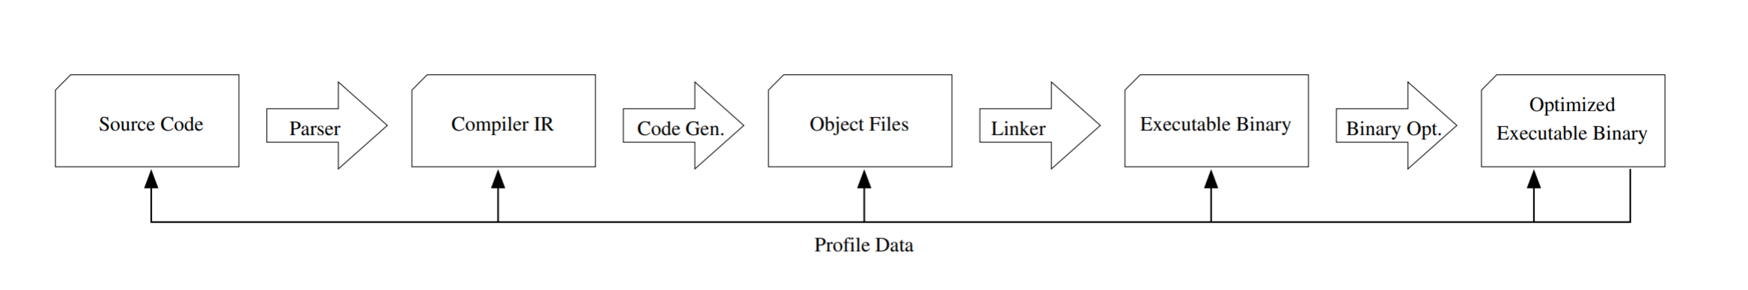
\includegraphics[width=1.0\linewidth]{translation}
    }
    \caption{Процесс трансляции исходного кода в оптимизированный бинарный файл}\label{fig:Compile}
\end{figure}

Оптимизация приложений является важнейшей частью процесса создания современного программного обеспечения, так как позволяет в разы повысить производительность и энергоэффективность вычислений. Оптимизации на основе профильной информации приложения позволяют получить большой прирост в указанных выше параметрах. Для получения профиля нужно использовать специально собранную версию приложения либо обеспечивать аппаратную поддержку сбора необходимых характеристик.

Для архитектуры x86 существует специальная аппаратная поддержка, позволяющая собирать профильную информацию во время исполнения приложения - LBR (Last Branch Record). Для ARM архитектуры аналог данной технологии существует, но не поддерживается всеми процессорами, что создаёт проблемы для оптимизаций приложений с учётом профиля исполнения. Произвести статическую инструментацию приложения не всегда является возможным, например, в случае отсутствия исходного кода или информации о символах и релокационных данных в бинарном файле. Поэтому \textbf{актуальной} задачей является разработка метода получения профильной информации для ARM архитектуры и дополнительных бинарных оптимизаций.

{\aim} данной работы является изучение и оптимизация существующих инструментов статической бинарной трансляции под RISC архитектуры. Основной целевой платформой является одна из наиболее распространенных на данный момент RISC архитектур -- ARM. Основным классом оптимизаций являются оптимизации, использующие профильную информацию исполнения приложения.

Для~достижения поставленной цели необходимо было решить следующие {\tasks}:
\begin{enumerate}[beginpenalty=10000] % https://tex.stackexchange.com/a/476052/104425
  \item Исследовать существующие статические бинарные трансляторы под RISC архитектуры.
  \item Разработать универсальный метод получения профильной информации под RISC архитектуры.
  \item Разработать ПО для получения профильной информации приложения по трассе его исполнения.
  \item Разработать методы улучшения статического бинарного транслятора.
  \item Реализовать наиболее перспективные методы улучшения бинарного оптимизатора.
  \item Разработать новые оптимизации на основе внедренных методов и улучшений.
  \item Протестировать разработанные методы на реальных приложениях под RISC архитектуру.
\end{enumerate}

Тема и содержание диссертационной работы соответствует паспорту научной специальности 05.13.11 – Математическое и программное обеспечение вычислительных машин, комплексов и компьютерных сетей, в частности, пунктам:

п. 1 – Модели, методы и алгоритмы проектирования и анализа программ и программных систем, их эквивалентных преобразований, верификации и тестирования.

п. 3 – Модели, методы, алгоритмы, языки и программные инструменты для организации взаимодействия программ и программных систем.

{\novelty}
\begin{enumerate}[beginpenalty=10000] % https://tex.stackexchange.com/a/476052/104425
  \item В диссертационной работе был реализован новый алгоритм получения профильной информации формата BOLT на основе трасс исполнения приложения. В диссертации показано, что для определенных классов устройств это единственный способ получения полноценного профиля приложения.
  \item Была реализована полноценная поддержка бинарного оптимизатора BOLT для ARM архитектуры, необходимая для проведения тестовых замеров на целевых приложениях, в то время как исходная версия BOLT не поддерживает оптимизацию нужных приложений.
  \item Был разработан специальный формат, описывающий преобразования исполняемого файла в оптимизированный.
  \item Был разработан статический анализатор, верифицирующий оптимизированный исполняемый файл на основе оригинального файла и файла преобразования.
  \item Был создан алгоритм мультипрофильного анализа, выделяющий профили приложения на основе трасс исполнения. На его основе реализована оптимизация копирования кода.

\end{enumerate}

{\influence} данной работы заключается в использовании разработанных методов и алгоритмов в бинарном оптимизаторе BOLT и его инфраструктуре и успешном \textbf{внедрении} компанией ООО <<Техкомпания Хуавэй>> для оптимизации приложений. Реализованные оптимизации, верификации и методы получения профильной информации позволили получить прирост производительности на целевых приложениях компании.

Результаты данной работы также \textbf{внедрены} в кафедральный курс «Современные методы разработки компиляторов» кафедры микропроцессорных технологий в интеллектуальных системах управления МФТИ.

Теоретическая значимость диссертационной работы заключается в разработке новых методов использования трасс исполнения приложения, как для получения профильной информации, так и для использования в анализе и оптимизациях.

{\defpositions}
\begin{enumerate}[beginpenalty=10000] % https://tex.stackexchange.com/a/476052/104425
  \item Метод получения профильной информации для бинарного оптимизатора BOLT из трасс исполнения приложений.
  \item Алгоритм оптимизации длинных переходов при работе бинарного оптимизатора BOLT.
  \item Алгоритм верификации оптимизированных бинарным оптимизатором BOLT файлов.
  \item Алгоритм мультипрофильного анализа трасс исполнения приложений.
  \item Алгоритм дублирования кода на основе мультипрофильного анализа трасс исполнения приложений.
\end{enumerate}

{\reliability}
Обоснованность и достоверность результатов и выводов диссертации подтверждается подробным описанием проведенных экспериментов и полученных данных.

{\probation}
Результаты диссертационной работы докладывались на следующих научно-технических конференциях:
\begin{enumerate}[beginpenalty=10000] % https://tex.stackexchange.com/a/476052/104425
  \item 63-й всероссийской научной конференции московского физико–технического института (государственного университета, Москва, ноябрь 2020 г.
  \item Международном конгрессе <<Современные проблемы компьютерных и информационных наук>>, Москва, ноябрь 2021 г.
  \item 64-й всероссийской научной конференции московского физико–технического института (государственного университета, Москва, ноябрь 2021 г.
\end{enumerate}

{\contribution} Основные результаты диссертационного исследования получены лично автором. Постановка задач и анализ полученных результатов осуществлялся непосредственно автором. В совместных работах вклад автора в результаты исследования являлся определяющим. Автор лично реализовывал и интегрировал разработанные решения в бинарный оптимизатор BOLT.

\ifnumequal{\value{bibliosel}}{0}
{%%% Встроенная реализация с загрузкой файла через движок bibtex8. (При желании, внутри можно использовать обычные ссылки, наподобие `\cite{vakbib1,vakbib2}`).
    {\publications} Основные результаты по теме диссертации изложены
    в~XX~печатных изданиях,
    X из которых изданы в журналах, рекомендованных ВАК,
    X "--- в тезисах докладов.
}%
{%%% Реализация пакетом biblatex через движок biber
    \begin{refsection}[bl-author, bl-registered]
        % Это refsection=1.
        % Процитированные здесь работы:
        %  * подсчитываются, для автоматического составления фразы "Основные результаты ..."
        %  * попадают в авторскую библиографию, при usefootcite==0 и стиле `\insertbiblioauthor` или `\insertbiblioauthorgrouped`
        %  * нумеруются там в зависимости от порядка команд `\printbibliography` в этом разделе.
        %  * при использовании `\insertbiblioauthorgrouped`, порядок команд `\printbibliography` в нём должен быть тем же (см. biblio/biblatex.tex)
        %
        % Невидимый библиографический список для подсчёта количества публикаций:
        \printbibliography[heading=nobibheading, section=1, env=countauthorvak,          keyword=biblioauthorvak]%
        \printbibliography[heading=nobibheading, section=1, env=countauthorwos,          keyword=biblioauthorwos]%
        \printbibliography[heading=nobibheading, section=1, env=countauthorscopus,       keyword=biblioauthorscopus]%
        \printbibliography[heading=nobibheading, section=1, env=countauthorconf,         keyword=biblioauthorconf]%
        \printbibliography[heading=nobibheading, section=1, env=countauthorother,        keyword=biblioauthorother]%
        \printbibliography[heading=nobibheading, section=1, env=countregistered,         keyword=biblioregistered]%
        \printbibliography[heading=nobibheading, section=1, env=countauthorpatent,       keyword=biblioauthorpatent]%
        \printbibliography[heading=nobibheading, section=1, env=countauthorprogram,      keyword=biblioauthorprogram]%
        \printbibliography[heading=nobibheading, section=1, env=countauthor,             keyword=biblioauthor]%
        \printbibliography[heading=nobibheading, section=1, env=countauthorvakscopuswos, filter=vakscopuswos]%
        \printbibliography[heading=nobibheading, section=1, env=countauthorscopuswos,    filter=scopuswos]%
        %
        \nocite{*}%
        %
        {\publications} Основные результаты по теме диссертации изложены в~\arabic{citeauthor}~печатных изданиях,
        \arabic{citeauthorvak} из которых изданы в журналах, рекомендованных ВАК\sloppy%
        \ifnum \value{citeauthorscopuswos}>0%
            , \arabic{citeauthorscopuswos} "--- в~периодических научных журналах, индексируемых Web of~Science и Scopus\sloppy%
        \fi%
        \ifnum \value{citeauthorconf}>0%
            , \arabic{citeauthorconf} "--- в~тезисах докладов.
        \else%
            .
        \fi%
        \ifnum \value{citeregistered}=1%
            \ifnum \value{citeauthorpatent}=1%
                Зарегистрирован \arabic{citeauthorpatent} патент.
            \fi%
            \ifnum \value{citeauthorprogram}=1%
                Зарегистрирована \arabic{citeauthorprogram} программа для ЭВМ.
            \fi%
        \fi%
        \ifnum \value{citeregistered}>1%
            Зарегистрированы\ %
            \ifnum \value{citeauthorpatent}>0%
            \formbytotal{citeauthorpatent}{патент}{}{а}{}\sloppy%
            \ifnum \value{citeauthorprogram}=0 . \else \ и~\fi%
            \fi%
            \ifnum \value{citeauthorprogram}>0%
            \formbytotal{citeauthorprogram}{программ}{а}{ы}{} для ЭВМ.
            \fi%
        \fi%
        % К публикациям, в которых излагаются основные научные результаты диссертации на соискание учёной
        % степени, в рецензируемых изданиях приравниваются патенты на изобретения, патенты (свидетельства) на
        % полезную модель, патенты на промышленный образец, патенты на селекционные достижения, свидетельства
        % на программу для электронных вычислительных машин, базу данных, топологию интегральных микросхем,
        % зарегистрированные в установленном порядке.(в ред. Постановления Правительства РФ от 21.04.2016 N 335)
    \end{refsection}%
    \begin{refsection}[bl-author, bl-registered]
        % Это refsection=2.
        % Процитированные здесь работы:
        %  * попадают в авторскую библиографию, при usefootcite==0 и стиле `\insertbiblioauthorimportant`.
        %  * ни на что не влияют в противном случае
        \nocite{vakbib1}%vak
        \nocite{vakbib2}%vak
        \nocite{confbib1}%conf
        \nocite{confbib2}%conf
        \nocite{confbib3}%conf
    \end{refsection}%
        %
        % Всё, что вне этих двух refsection, это refsection=0,
        %  * для диссертации - это нормальные ссылки, попадающие в обычную библиографию
        %  * для автореферата:
        %     * при usefootcite==0, ссылка корректно сработает только для источника из `external.bib`. Для своих работ --- напечатает "[0]" (и даже Warning не вылезет).
        %     * при usefootcite==1, ссылка сработает нормально. В авторской библиографии будут только процитированные в refsection=0 работы.
} % Характеристика работы по структуре во введении и в автореферате не отличается (ГОСТ Р 7.0.11, пункты 5.3.1 и 9.2.1), потому её загружаем из одного и того же внешнего файла, предварительно задав форму выделения некоторым параметрам
\newpage
\textbf{Объем и структура работы.} Диссертация состоит из~введения,
\formbytotal{totalchapter}{глав}{ы}{}{},
заключения и
\formbytotal{totalappendix}{приложен}{ия}{ий}{}.
%% на случай ошибок оставляю исходный кусок на месте, закомментированным
%Полный объём диссертации составляет  \ref*{TotPages}~страницу
%с~\totalfigures{}~рисунками и~\totaltables{}~таблицами. Список литературы
%содержит \total{citenum}~наименований.
%
Полный объём диссертации составляет
\formbytotal{TotPages}{страниц}{у}{ы}{}, включая
\formbytotal{totalcount@figure}{рисун}{ок}{ка}{ков} и
\formbytotal{totalcount@table}{таблиц}{у}{ы}{}.
Список литературы содержит
\formbytotal{citenum}{наименован}{ие}{ия}{ий}.
    % Введение
\ifnumequal{\value{contnumfig}}{1}{\counterwithout{figure}{chapter}
}{\counterwithin{figure}{chapter}}
\ifnumequal{\value{contnumtab}}{1}{\counterwithout{table}{chapter}
}{\counterwithin{table}{chapter}}
\chapter{Обзор существующих технологий бинарной трансляции}\label{ch:ch1}
Первая глава содержит обзор существующих технологий бинарных трансляторов, используемых для генерации оптимизированных исполняемых файлов приложений.

В разделе 1.1 приводится описание методов оптимизаций приложений.

В разделе 1.2 рассматриваются общие принципы работы существующих технологий бинарных оптимизаторов и приводится обзор на существующие решения.

В разделе 1.3 подробно рассматривается устройство бинарного оптимизатора BOLT (Binary Optimization and Layout Tool), вопросы получения профильной информации для его работы на x86 архитектуре с использованием аппаратной поддержки профилирования -- LBR (Last Branch Record).

Разбираются вопросы формата профилей с информацией о взятых переходах и без неё и пример оптимизации простого приложения с условным переходом в цикле.

В конце первой главы обсуждается вопрос поддержки архитектуры ARM в бинарном оптимизаторе BOLT, варианты получения профильной информации на ней и возможности оптимизаций. Приведены примеры профилей в формате BOLT.

\section{Процесс оптимизации приложений}\label{sec:ch1/sec1}
На данный момент большинство программ пишутся на языке программирования высокого уровня, после чего применяются трансляторы, переводящие их в бинарный формат (рисунок \cref{fig:TransVar}). Так называемые программирующие программы (компиляторы) появились ещё в 50-х годах двадцатого века.

\begin{figure}[!h]
    \centerfloat{
        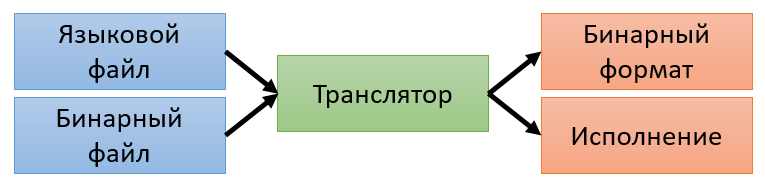
\includegraphics[width=0.8\linewidth]{translate1}
    }
    \caption{Варианты работы транслятора}\label{fig:TransVar}
\end{figure}

Практически всегда приложение проходит процесс оптимизации во время компиляции, так как данные проходы включают в системах сборки по умолчанию. Во время трансляции программы с языка высокого уровня в бинарный код реальной или виртуальной машины получаемое промежуточное представление подвергается упорядоченному набору оптимизаций. Для компилируемых языков применяются дополнительные оптимизации времени компоновки кода (LTO – Link Time Optimizations), поскольку на этом этапе становится доступно больше информации о всех полученных объектных файлах. После компоновки кода приложение готово к использованию \cite{Wu1994}. Для данных оптимизаций использовалась информация о приложении, полученная из исходного кода.

Для повышения производительности можно собрать профиль исполнения приложения, что позволит лучше подобрать эвристики для используемых оптимизационных проходов, а также применить дополнительные проходы в компиляторе и линкере \cite{Licker2020}.

\section{Бинарная оптимизация}\label{sec:ch1/sec2}
В случае, когда доступа к исходному коду нет, но есть бинарный файл приложения и его профиль исполнения, появляется возможность провести бинарную оптимизацию\cite{Li2019}. Тогда на вход транслятору будет подаваться не языковой, а бинарный файл (рисунок \cref{fig:TransVar}), который будет переведён в другой бинарный формат.

Целевая архитектура для входного и выходного формата могут не совпадать. В случае их совпадения целесообразно использовать данный транслятор с оптимизациями под конкретную модель процессора. Добавив информацию о его спецификации, на котором будет исполнятся приложение, можно провести ряд микроархитектурных оптимизаций. Также можно использовать профильную информацию исполнения для проведения дополнительных оптимизирующих проходов.

За последние несколько лет наблюдается резкий рост популярности бинарных оптимизаторов: BOLT \cite{Panchenko2019}, Propeller \cite{Moreira2021}, Janus \cite{Zhou2019}, HALO \cite{Savage2020}, Ispike \cite{Luk2004}. Эти инструменты используют профильную информацию исполнения для принятия решений по оптимизации.

Оптимизация, основанная на обратной связи (FDO, Feedback Directed Optimization), является эффективным методом повышения производительности программ сверх того, что обычно могут достичь статические компиляторы \cite{Chen2016}. В данном сценарии компилятор использует информацию, полученную в результате предыдущих исполнений целевой программы, для выполнения более агрессивных преобразований кода. FDO является ключевым компонентом инструментов бинарной оптимизации, которые полагаются на информацию профилирования для выполнения преобразований, таких как изменение порядка базовых блоков и функций.
Эти инструменты достигают прироста производительности благодаря оптимизации с профилем исполнения: BOLT (Binary Optimization and Layout Tool) \cite{Panchenko2019} дает ускорение приложений до 30\% (при отсутствии предварительных профильных оптимизаций).

Несмотря на эффективность, сбор данных во время выполнения создает разработчикам неудобства: подбор входных данных, необходимость внесения изменений в программное обеспечение и увеличение времени сборки.

Помимо генерации бинарного файла, транслятор может произвести исполнение считанного им кода на высокоуровневом языке программирования либо бинарном формате. В первом случае это будет интерпретацией, во втором - моделированием/бинарной интерпретацией, что позволяет проводить тестовые запуски без наличия реального устройства.

\section{Обзор бинарного оптимизатора BOLT}\label{sec:ch1/sec3}
Основными целевыми приложениями для оптимизатора BOLT являются современные программы для центров обработки данных. Из-за размера кода программ повышение его локализации стало важным инструментом повышения производительности \cite{Ottoni2017}. Основной оптимизацией BOLT является перекомпоновка кода на основе полученного профиля, использование которого на бинарном уровне точнее, чем на этапе компиляции (рисунок \cref{fig:BOLT}) \cite{Newell2020}. Создатели данного бинарного оптимизатора достигли прироста производительности в 10\% на x86 приложениях, скомпилированные с оптимизациями времени связывания и с использованием профиля \cite{Panchenko2019}\cite{Panchenko2021}.

\begin{figure}[!h]
    \centerfloat{
        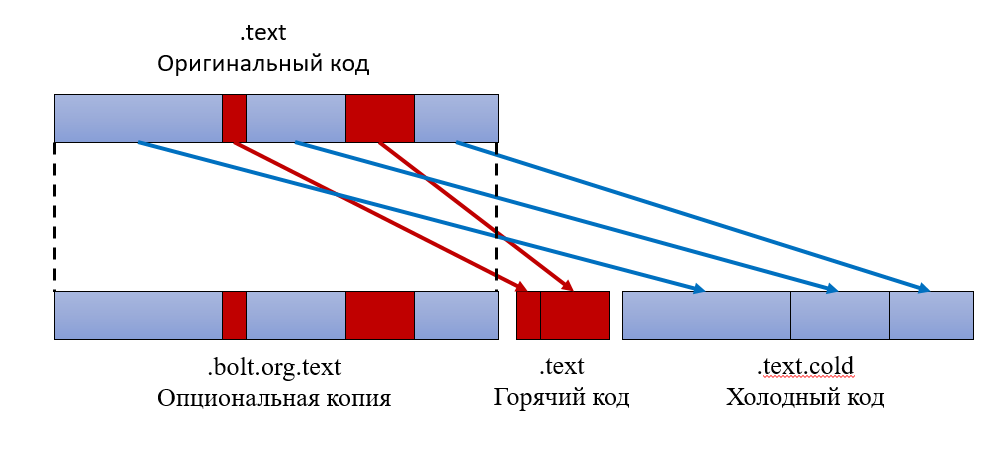
\includegraphics[width=1.0\linewidth]{1}
    }
    \caption{Алгоритм работы бинарного оптимизатора BOLT}\label{fig:BOLT}
\end{figure}

Данный бинарный оптимизатор написан с использованием фреймворка генерации компиляторов – LLVM \cite{Lattner2004}, что делает BOLT потенциально портируемым на множество других архитектур. Базовая поддержка ARM архитектуры (Aarch64) на данный момент уже добавлена.

BOLT применим к приложениям, размер которых значительно больше размера L1I (инструкционного кэша 1 уровня) и размера отображаемого кода iTLB (буфер ассоциативной трансляции инструкций) - десятки мегабайт и более. За счет новой компоновки кода, основанной на профиле, часто исполняемый код локализуется в новой секции. Частоту исполнения кода называют его <<температурой>>, и в данном примере созданная секция является <<горячей>>. Остальной же код с меньшей частотой исполнения будет называться <<холодным>>. Теперь при обращении в горячий участок кода в кэш-линию, помимо исполняемого в данный момент кода, будут попадать более горячие соседние участки из новой секции, и температура кода инструкционного кэша будет выше \cite{Lavaee2019}. Это приводит к меньшим промахам при обращении в L1I и iTLB, а значит к повышению производительности.

Для оптимизации с помощью BOLT необходима релокационная информация, так как его алгоритм производит перекомпоновку всей секции .text, в которой может содержаться как код, так и данные. Это одна из особенностей фон-Неймановских архитектур: код и данные располагаются в одном адресном пространстве.

На рисунке \cref{fig:4byte} представлен пример, когда одни и те же 4-байтовые данные могут обозначать либо ARM инструкцию условного перехода, либо 4 символа. При перекомпоновке необходимо изменить значение смещения инструкции b.ls, во втором случае 4-байтовые данные должны остаться неизменными, поэтому без дополнительной информации о расположении данных оптимизатор не сможет решить, как обработать секцию корректно. 

\begin{figure}[!h]
    \centerfloat{
        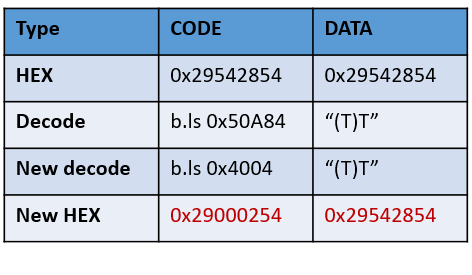
\includegraphics[width=0.7\linewidth]{12}
    }
    \caption{Пример модификации 4-байтовых данных при перемещении кода}\label{fig:4byte}
\end{figure}

Помимо релокационной информации BOLT требует наличие символов в бинарном файле, так как он оперирует с бинарными функциями. Также формат профиля в BOLT использует имена символов для обозначения местоположения инструкций переходов.

\subsection{Получение профильной информации для оптимизатора BOLT}\label{subsec:ch1/sec3/sub1}
Один из способов собрать профиль – провести инструментацию бинарного файла \cite{Ottoni2018}. Во время запуска будет произведена запись по счетчикам, расставленным во время компиляции, но для данного подхода необходим исходный код. Основная проблема заключается в необходимости адаптации инфраструктуры сборки проекта для профилирования. Кроме того, используемые сторонние библиотеки не предоставляются в инструментированном виде, что осложняет получения полной картины исполнения \cite{Nethercote2007}.

Вместо инструментации кода во время компиляции разработаны среды, позволяющие произвести инструментацию во время исполнения приложения. Таким образом, может быть получена вся необходимая информация об исполнении при разрешении сложностей извлечения собранных данных. Однако, стоимость разработки динамической инструментации выше разработки аналогичного процесса в момент компиляции. Также появляются затраты вычислительных ресурсов во время записи трасс исполнения.\cite{Li2007}

При наличии архитектурной поддержки есть возможность собрать информацию исполнения с меньшими расходами. В x86 архитектуре такая поддержка есть, что позволило сотрудникам Facebook использовать такой подход в своём бинарном оптимизаторе BOLT (рисунок \cref{fig:OptX86})\cite{Panchenko2019}.

\begin{figure}[!h]
    \centerfloat{
        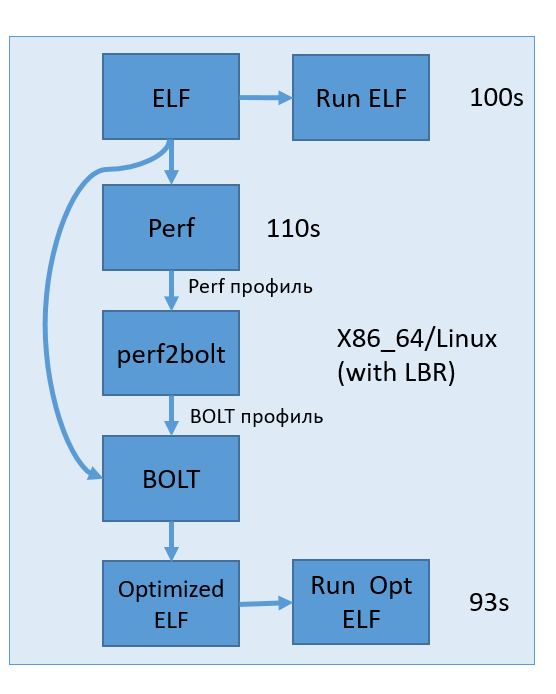
\includegraphics[width=0.6\linewidth]{2}
    }
    \caption{Схема оптимизации бинарного файла на x86 архитектуре}\label{fig:OptX86}
\end{figure}

Для нахождения горячих и холодных участков кода используется профиль (рисунок \cref{fig:ProfileFormat}), собранный на основе выборок. BOLT использует данные, полученные с помощью приложения perf, собирающее статистические данные исполнения, такие как значения счетчика команд и последние взятые переходы с информацией от предсказателя переходов. Последний параметр предоставляется perf благодаря аппаратной поддержке в архитектуре x86. Поддержка осуществляется с помощью LBR (Last Branch Record), записывающей информацию о последних 8-32 (в зависимости от модели процессора) переходах.

\begin{figure}[!h]
    \centerfloat{
        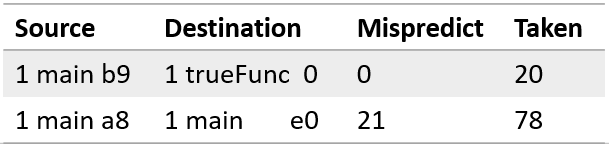
\includegraphics[width=0.8\linewidth]{profile}
    }
    \caption{Формат профильной информации бинарного оптимизатора BOLT}\label{fig:ProfileFormat}
\end{figure}

Сначала идет информация о местонахождении инструкции перехода (Source). Это поле задается тремя значениями: является ли дальнейшее поле символом (0 или 1), имя символа в исполняемом файле, смещение от символа  до инструкции перехода. Далее в такой же последовательности следует информация о месте назначения прыжка (Destination). Последние два числа – количество не предсказанных и количество взятых переходов.
	На рисунке \cref{fig:ProfileFormat} продемонстрирована информация о двух переходах:
	
\begin{enumerate}[beginpenalty=10000]
  \item Вызов trueFunc из main, являющийся прямым прыжком (поэтому mispredict = 0), взятый 20 раз.
  \item Переход внутри функции main, который является условным прыжком, не предсказанный 21 раз и взятый 78 раз.
\end{enumerate}

Затем происходит конвертация профиля из формата perf в формат BOLT при помощи приложения perf2bolt. В итоге будет сгенерирован список записей, состоящих из адресов начала и конца перехода, количества не предсказанных и количества взятых переходов.

На основании полученного профиля начинается работа бинарного оптимизатора. На рисунке \cref{fig:BinOptSteps} представлена схема работы BOLT.

\begin{figure}[!h]
    \centerfloat{
        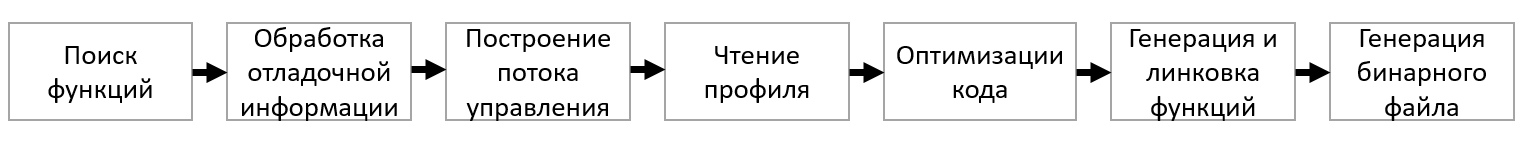
\includegraphics[width=1.0\linewidth]{3}
    }
    \caption{Последовательность работы бинарного оптимизатора BOLT}\label{fig:BinOptSteps}
\end{figure}

Уровни абстракций, на которых работает BOLT, выстраиваются в последовательности, показанной на рисунке \cref{fig:BOLTAbst}.

\begin{figure}[!h]
    \centerfloat{
        
\includegraphics[width=1.0\linewidth]{4}
    }
    \caption{Уровни абстракции бинарного оптимизатора BOLT}\label{fig:BOLTAbst}
\end{figure}

Для первых 4 абстракций создатели BOLT написали в программном коде свои собственные классы. Машинные инструкции были использованы из стандартных классов LLVM (MCInst). Под бинарным базовым блоком понимается линейный участок кода, исполнение которого всегда идёт с его первой инструкции и заканчивается последней.

После работы бинарного оптимизатора получается новый бинарный файл, в котором вместо одной секции .text с исходным кодом появляется две секции .text (с горячим кодом) и .text.cold (с холодным кодом).
	
BOLT поддерживает возможность сохранения оригинальной секции. В таком случае он переименует её в .bolt.org.text. Это необходимо для тех случаев, когда перенос некоторых бинарных функций невозможен и необходимо переиспользовать оригинальный код.


\subsection{Пример оптимизации}\label{subsec:ch1/sec3/sub2}

Рассмотрим пример оптимизации следующей функции main (рисунок \cref{fig:TestCode}).

\begin{figure}[!h]
    \centerfloat{
        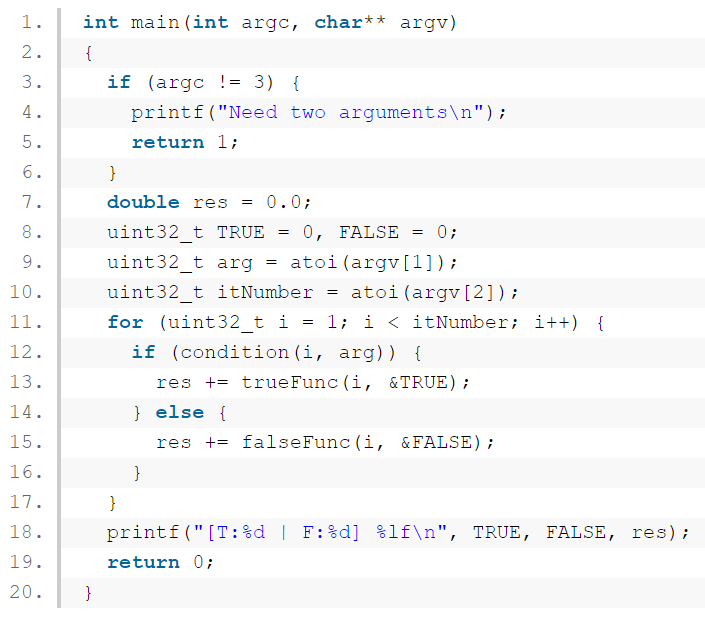
\includegraphics[width=0.8\linewidth]{5}
    }
    \caption{Пример оптимизируемого демонстрационного приложения}\label{fig:TestCode}
\end{figure}

BOLT найдёт символ main в таблице символов, перейдёт по указанному адресу в бинарном файле, дизассемблирует тело функции и выстроит поток управления данной функции (рисунок \cref{fig:CFG}).

\begin{figure}[!h]
    \centerfloat{
        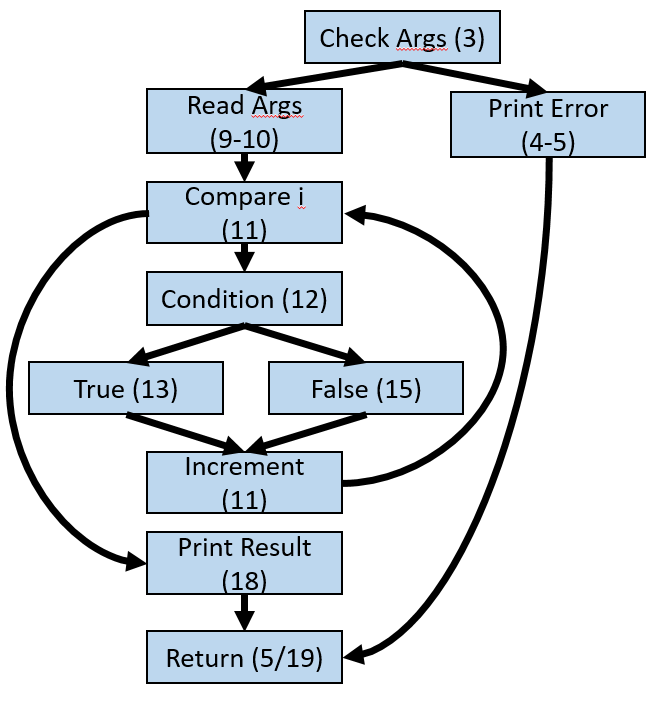
\includegraphics[width=0.6\linewidth]{6}
    }
    \caption{Граф потока управления (в скобках соответствующие строки кода)}\label{fig:CFG}
\end{figure}

Каждому узлу в графе потока управления соответствует один бинарный базовый блок, которым будет оперировать BOLT. При компиляции без профильной информации компилятор размещает код последовательно в одной .text секции, как указано на рисунке \cref{fig:BBOpt} слева. После запуска программы с профилировщиком на конкретных аргументах получим следующий профиль (рисунок \cref{fig:CFGProfile}).

\begin{figure}[!h]
    \centerfloat{
        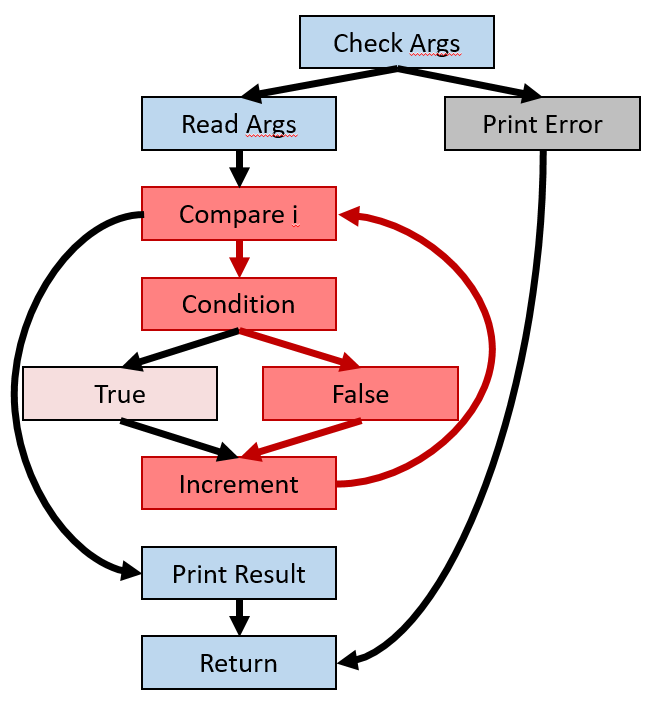
\includegraphics[width=0.6\linewidth]{7}
    }
    \caption{Граф потока управления с профильной информацией}\label{fig:CFGProfile}
\end{figure}

С учетом полученной информации от профилировщика известна частота исполнения базовых блоков, размещенных в бинарном файле (рисунок \cref{fig:BBOpt}, в центре). Получается, что самый часто исполняемый (горячий код) разбит холодным бинарным базовым блоком True, который будет попадать в кэш-линию при копировании кода в L1I и понижать его среднюю температуру.

\begin{figure}[!h]
    \centerfloat{
        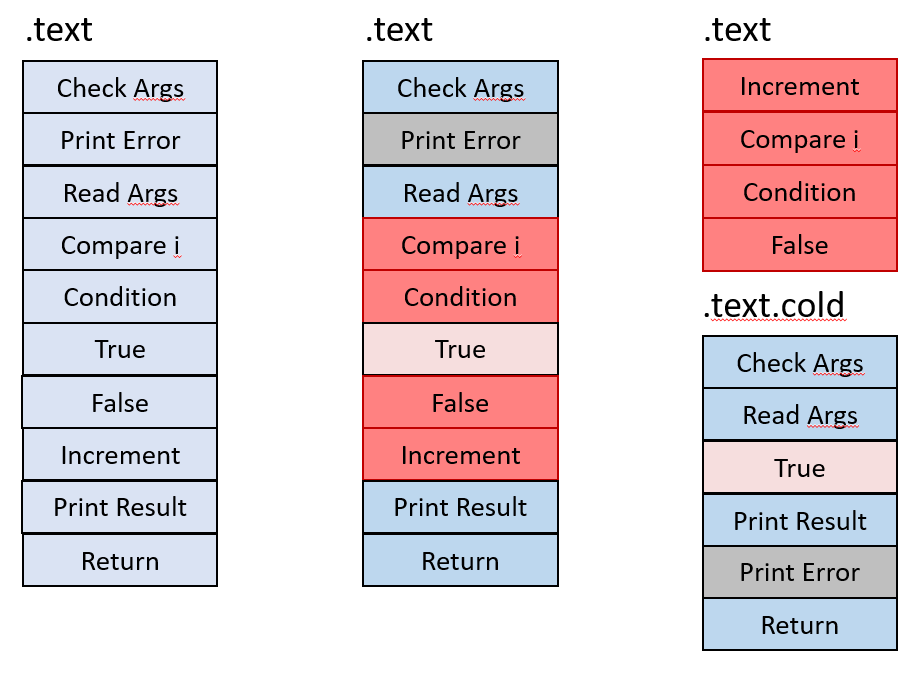
\includegraphics[width=0.8\linewidth]{8}
    }
    \caption{Расположение базовых блоков в секции (без профильной информации – с профильной информацией – после перекомпоновки кода)}\label{fig:BBOpt}
\end{figure}

Оптимизация BOLT переставляет бинарные базовые блоки (рисунок \cref{fig:BBOpt}, справа). Самые горячие блоки попадут в горячую секцию .text, остальные будут скопированы в секцию .text.cold. В итоге за счёт повышения средней температуры L1I  и iTLB полученный бинарный файл будет работать быстрее.

Как было сказано раньше, основной архитектурой для оптимизации была заявлена x86. Также заявлена поддержка 64-битной ARM архитектуры (Aarch64), но на деле возникает множество проблем при попытке использования оптимизатора на ней. Они будут рассмотрены в следующих разделах.


\subsection{Результаты тестирования BOLT на архитектуре x86}\label{subsec:ch1/sec3/sub3}
Для приведенного кода (рисунок \cref{fig:TestCode}) был получен профиль на x86 архитектуре с (таблица \cref{tab:X86LBR}) и без (таблица \cref{tab:X86noLBR}) информацией о взятых переходах из LBR.

no\_LBR\_mode – режим сбора статистики без LBR, в котором профильная информация включает в себя только количество исполнений конкретных инструкций.
\begin{table} [!h]% Пример записи таблицы с номером, но без отображаемого наименования
    \centering
    \begin{threeparttable}% выравнивание подписи по границам таблицы
        \caption{Профиль демонстрационного примера на x86 архитектуре, собранного с учетом информации из LBR}%
        \label{tab:X86LBR}%
        \begin{SingleSpace}
            \begin{tabular}{| c | c | c | c | c | c | c | c |}
                \hline
                	1 & main &      75 & 1 & main &      7b & 0 &   452 \\ \hline
				1 & main &      9e & 1 & main &      a4 & 0 &   421 \\ \hline
				1 & main &      ec & 1 & main &      f1 & 0 &   331 \\ \hline
				1 & main &      e2 & 1 & falseFunc & 0 &  0 &   665 \\ \hline
				1 & main &      c8 & 1 & main &      f1 & 0 &   98 \\ \hline
				1 & main &      9e & 1 & main &      cd & 317 &  730 \\ \hline
				1 & main &      b9 & 1 & trueFunc &  0 &  0 &   159 \\ \hline
				1 & main &      f1 & 1 & main &      f6 & 0 &   494 \\ \hline
				1 & main &      96 & 1 & condition & 0 &  0 &   4535 \\ \hline
				1 & main &      ff & 1 & main &      6e & 0 &   490 \\ \hline
				1 & main &      8c & 1 & atoi@PLT &  0 &  0 &   468 \\ \hline
				0 & [unknown] & 0 &  1 & main &      91 & 0 &   4346 \\ \hline
				1 & falseFunc & 1e & 1 & falseFunc & 25 & 0 &   569 \\ \hline
				1 & falseFunc & 2b & 1 & falseFunc & 31 & 0 &   2558 \\ \hline
				1 & falseFunc & 2b & 1 & falseFunc & 5f & 303 & 378 \\ \hline
				1 & falseFunc & 5a & 1 & falseFunc & 25 & 0 &   2657 \\ \hline
				1 & falseFunc & 65 & 1 & main &      e7 & 0 &   372 \\ \hline
				1 & condition & 7b & 1 & main &      9b & 1 &   891 \\ \hline
				1 & condition & 38 & 1 & sin@PLT &   0 &  0 &   4695 \\ \hline
				0 & [unknown] & 0 &  1 & condition & 3d & 1 &   1528 \\ \hline
				1 & sin@PLT &   0 &  0 & [unknown] & 0 &  34 &  4826 \\ \hline
				1 & trueFunc &  1e & 1 & trueFunc &  25 & 0 &   147 \\ \hline
				1 & trueFunc &  2b & 1 & trueFunc &  31 & 0 &   656 \\ \hline
				1 & trueFunc &  2b & 1 & trueFunc &  5f & 83 &  105 \\ \hline
				1 & trueFunc &  65 & 1 & main &      be & 0 &   102 \\ \hline
				1 & trueFunc &  5a & 1 & trueFunc &  25 & 0 &   678 \\ \hline
				1 & atoi@PLT &  0 &  0 & [unknown] & 0 &  9 &   541 \\ \hline

            \end{tabular}%
        \end{SingleSpace}
    \end{threeparttable}
\end{table}

\begin{table} [!h]% Пример записи таблицы с номером, но без отображаемого наименования
    \centering
    \begin{threeparttable}% выравнивание подписи по границам таблицы
        \caption{Профиль демонстрационного примера на x86 архитектуре, собранного без учета информации от LBR}%
        \label{tab:X86noLBR}%
        \begin{SingleSpace}
            \begin{tabular}{| c | c | c | c | c | c | c | c | c |}
            \hline
			1& main&      b3& 2 & &
			1& main&      de& 4 \\ \hline
			1& main&      75& 1 & &
			1& main&      6e& 13 \\ \hline
			1& main&      a9& 3 & &
			1& main&      7e& 5 \\ \hline
			1& main&      7b& 1 & &
			1& main&      ec& 34 \\ \hline
			1& main&      89& 1 & &
			1& main&      e2& 12 \\ \hline
			1& main&      dc& 1 & &
			1& main&      d9& 47 \\ \hline
			1& main&      c3& 3 & &
			1& main&      8c& 6 \\ \hline
			1& main&      f1& 4 & &
			1& main&      e7& 7 \\ \hline
			1& main&      ff& 11 & &
			1& main&      be& 1 \\ \hline
			1& main&      f6& 9 & &
			1& main&      82& 14 \\ \hline
			1& main&      b0& 9 & &
			1& main&      cd& 15 \\ \hline
			1& main&      d0& 8 & &
			1& condition& 33& 11 \\ \hline
			1& condition& 7b& 16 & &
			1& condition& 47& 4 \\ \hline
			1& condition& 8&  1 & &
			1& condition& 6d& 136 \\ \hline
			1& condition& 70& 38 & &
			1& condition& 73& 22 \\ \hline
			1& condition& 5e& 49 & &
			1& condition& 0 & 11 \\ \hline
			1& condition& 2b& 6 & &
			1& condition& 4c& 9 \\ \hline
			1& condition& 3d& 10 & &
			1& condition& 26& 14 \\ \hline
			1& condition& 1b& 20 & &
			1& condition& 63& 18 \\ \hline
			1& condition& 4 & 14 & &
			1& condition& 55& 406 \\ \hline
			1& falseFunc& f & 7 & &
			1& falseFunc& 16& 10 \\ \hline
			1& falseFunc& 19& 1 & &
			1& falseFunc& 51& 20 \\ \hline
			1& falseFunc& 3c& 25 & &
			1& falseFunc& 4c& 85 \\ \hline
			1& falseFunc& 25& 34 & &
			1& falseFunc& 4 & 9 \\ \hline
			1& falseFunc& 5a& 6 & &
			1& falseFunc& 57& 6 \\ \hline
			1& falseFunc& 43& 22 & &
			1& falseFunc& 3e& 14 \\ \hline
			1& falseFunc& 1 & 1 & &
			1& falseFunc& 64& 12 \\ \hline
			1& falseFunc& 54& 4 & &
			1& falseFunc& 39& 9 \\ \hline
			1& falseFunc& 47& 99 & &
			1& falseFunc& 31& 19 \\ \hline
			1& falseFunc& b & 9 & &
			1& falseFunc& 5f& 12 \\ \hline
			1& falseFunc& 28& 9 & &
			1& trueFunc&  43& 1 \\ \hline
			1& trueFunc&  25& 8 & &
			1& trueFunc&  5f& 3 \\ \hline
			1& trueFunc&  57& 5 & &
			1& trueFunc&  0 & 6 \\ \hline
			1& trueFunc&  3c& 16 & &
			1& trueFunc&  64& 2 \\ \hline
			1& trueFunc&  5a& 1 & &
			1& trueFunc&  3e& 1 \\ \hline
			1& trueFunc&  4c& 14 & &
			1& trueFunc&  31& 4 \\ \hline
			1& trueFunc&  51& 9 & &
			1& trueFunc&  f & 1 \\ \hline
			1& trueFunc&  7 & 7 & &
			1& trueFunc&  47& 23 \\ \hline
			1& trueFunc&  14& 1 & &
			1& atoi@PLT&  0 & 13 \\ \hline
            \end{tabular}%
        \end{SingleSpace}
    \end{threeparttable}
\end{table}

На данном приложении удалось получить 10\% прирост производительности на x86 архитектуре. Прирост производительности без информации из LBR был в два раза ниже.

\subsection{Поддержка ARM архитектуры бинарным оптимизатором}\label{subsec:ch1/sec3/sub4}
Основной проблемой при использовании ARM архитектуры является отсутствие стандартного подхода для сбора профилировочной информации. Для использования BOLT предлагается использовать no\_LBR\_mode. При этом согласно статье разработчиков BOLT и тестированию, информации профиля будет недостаточно для полноценного получения прироста производительности с помощью оптимизатора \cite{Panchenko2019}.


\begin{table} [h]% Пример записи таблицы с номером, но без отображаемого наименования
    \centering
    \begin{threeparttable}% выравнивание подписи по границам таблицы
        \caption{Профиль демонстрационного примера на ARM архитектуре, собранного в режиме no LBR}%
        \label{tab:ARMnoLBR}%
        \begin{SingleSpace}
            \begin{tabular}{| c | c | c | c | c | c | c | c | c |}
            \hline
			1& main& 94& 1 & &
			1& main& cc& 4 \\ \hline
			1& main& 9c& 1 & &
			1& main& 80& 7 \\ \hline
			1& main& a0& 14 & &
			1& main& e0& 106 \\ \hline
			1& main& e4& 4 & &
			1& main& 100& 21 \\ \hline
			1& main& 74& 52 & &
			1& main& 11c& 16 \\ \hline
			1& main& 7c& 20 & &
			1& main& ec& 6 \\ \hline
			1& main& 118& 8 & &
			1& main& d4& 4 \\ \hline
			1& main& ac& 20 & &
			1& main& 108& 3 \\ \hline
			1& condition& 48& 1 & &
			1& condition& 14& 2 \\ \hline
			1& condition& 34& 4 & &
			1& condition& 1c& 1 \\ \hline
			1& condition& 64& 111 & &
			1& condition& 60& 356 \\ \hline
			1& condition& 8 &2 & &
			1& condition& 18& 15 \\ \hline
			1& condition& 20& 7 & &
			1& condition& 44& 63 \\ \hline
			1& condition& 3c& 7 & &
			1& condition& 30& 1 \\ \hline
			1& condition& 50& 2 & &
			1& condition& 24& 3 \\ \hline
			1& falseFunc& 5c& 4 & &
			1& falseFunc& 38& 2 \\ \hline
			1& falseFunc& 58& 42 & &
			1& falseFunc& 54& 2 \\ \hline
			1& falseFunc& 3c& 49 & &
			1& falseFunc& 68& 79 \\ \hline
			1& falseFunc& 18& 3 & &
			1& falseFunc& 30& 44 \\ \hline
			1& falseFunc& 40& 3 & &
			1& falseFunc& 14& 4 \\ \hline
			1& falseFunc& 1c& 13 & &
			1& falseFunc& 20& 3 \\ \hline
			1& falseFunc& 4c& 207 & &
			1& falseFunc& 2c& 2 \\ \hline
			1& trueFunc& 1c& 2 & &
			1& trueFunc& 4c& 42 \\ \hline
			1& trueFunc& 3c& 13 & &
			1& trueFunc& 20& 1 \\ \hline
			1& trueFunc& 68& 26 & &
			1& trueFunc& 2c& 1 \\ \hline
			1& trueFunc& 30& 15 & &
			1& trueFunc& 58& 15 \\ \hline

            \end{tabular}%
        \end{SingleSpace}
    \end{threeparttable}
\end{table}


Для ARMv8 есть расширения для серверных процессоров, которые близки по функциональности к LBR, но отсутствуют на других, например, на мобильных процессорах. Также в ARM архитектуре предусмотрен ETM (ARM Embedded Trace Macrocell), позволяющий собрать нужную для профиля информацию, но его использование в пользовательском режиме не представляется возможным. Поэтому предлагается иной подход к сбору профильной информации \cite{Fu2018}.

Альтернативный способ получения профиля (no\_LBR\_mode) – это сбор значений программного счетчика (таблица \cref{tab:ARMnoLBR}). С их помощью собирается информация о частоте исполнения кода в процессе исполнения. Однако, такой подход не позволяет использовать весь список оптимизаций, включенных в BOLT. Данный способ применяется аналогично с использованием инструмента perf.

Столкнувшись с проблемой неполноценной оптимизации на ARM архитектуре, было принято решение разработать метод получения полноценного профиля с использованием динамической бинарной инструментации.

\clearpage
           % Глава 1
\chapter{Получение профильной информации из трасс исполнения}\label{ch:ch2}

В данной главе рассматривается разработанный универсальный метод получения профильной информации приложения из трасс исполнения.

В разделе 2.1 описывается метод получения трасс исполнения приложений на основе динамической бинарной инструментации и приводится предлагаемая схема оптимизации бинарного файла на ARM архитектуре.

В разделе 2.2 изложен алгоритм работы модели предсказателя переходов по трассе исполнения приложения, необходимый для получения информации о промахах предсказателя для профиля.

В разделе 2.3 приводится сравнение предлагаемого решения с уже существующим подходом работы бинарного оптимизатора BOLT. Сопоставляются профили, полученные на ARM и x86 архитектурах. Сравниваются подходы получения профильной информации с помощью аппаратной поддержки LBR и трасс исполнения приложения.

В разделе 2.4 описываются используемые синтетические тесты для проверки корректности работы предлагаемого метода получения профильной информации.

В разделе 2.5 приводятся результаты запусков оптимизированных на основе профильной информации, собранной из трасс исполнения, синтетических тестов.

\section{Получение трасс исполнения приложений}\label{sec:ch2/sec2}
Для анализа исполняемого файла без исходного кода применяется динамическая бинарная инструментация (DBI, Dynamic Binary Instrumentation). Во время работы приложения производится модификация программы с целью её анализа. С помощью инструментирующих процедур происходит вставка дополнительного кода \cite{Nethercote2007}. Это позволяет производить анализ во время возникновения в программе необходимых событий, таких как исключения, взятие переходов, создание процессов и т.д. \cite{Li2007}.

На основе данного подхода были реализованы DBI фреймворки, такие как Valgring \cite{Nethercote2003}, PIN, DynamoRIO \cite{Bruening2003} и DynInst \cite{Rimsa2019}. На их основе реализуются динамические бинарные анализаторы (DBA, Dynamic Binary Analysis), один из них был использован для сбора профильной информации для ARM архитектуры\cite{Hazelwood2006}. 

С помощью DBI фреймворка производится запись трассы исполнения приложения \cite{Hong2019}. Записывается последовательность инструкций, поступающих на процессор. После исполнения последовательность анализируется конвертером для генерации профиля исполнения, который записывается в формате BOLT (рисунок \cref{fig:NewSteps}). Такое решение приводит к замедлению работы оптимизируемого приложения в несколько раз, но создаёт трассу, которую можно анализировать без привязки к конкретной микроархитектуре. \cite{vakbib1} \cite{confbib2}

\begin{figure}[ht]
    \centerfloat{
        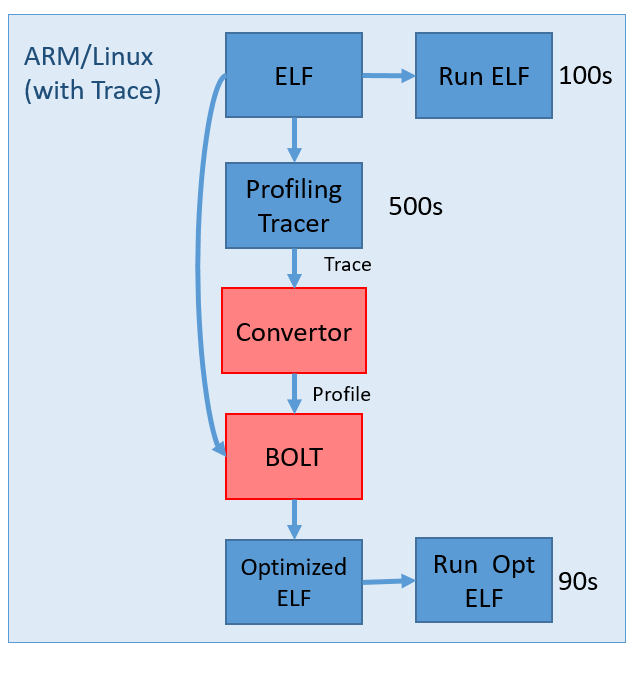
\includegraphics[width=0.6\linewidth]{9}
    }
    \caption{Предлагаемая схема оптимизации бинарного файла на ARM архитектуре}\label{fig:NewSteps}
\end{figure}

\section{Моделирование предсказателя переходов}\label{sec:ch2/sec3}
Чтобы получить информацию о переходах для профиля, конвертер проходит по всей трассе и находит инструкции меняющие поток управления: B, BR, BL, BLR, B.cond, TBZ, TBNZ, CBZ, CBNZ, RET (рисунок \cref{fig:ProfilefromTrace}) \cite{Kalla2017}. После чего информация поступает в модель предсказателя переходов (Branch Predictor Model). Данная модель выбирается в зависимости от конкретной микроархитектуры процессора, для которого оптимизируется приложение. В итоге собирается информация для получения количества не предсказанных и количества взятых переходов \cite{Ball1993} \cite{Fisher1992}.

\begin{figure}[ht]
    \centerfloat{
        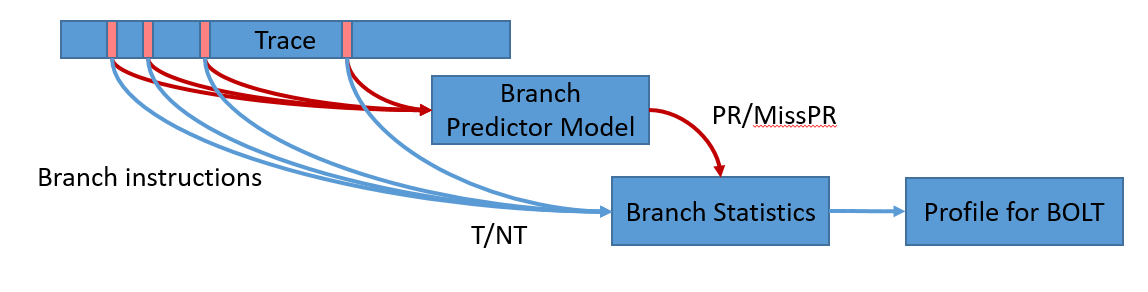
\includegraphics[width=1.0\linewidth]{10}
    }
    \caption{Схема генерации профиля из трассы исполнения}\label{fig:ProfilefromTrace}
\end{figure}

Для используемых в рамках данной работы устройств была реализована модель обрабатывающая три типа событий:
\begin{enumerate}[beginpenalty=10000]
  \item Безусловный переход по адресу.
  \item Условный переход по адресу.
  \item Косвенный переход по регистру.
\end{enumerate}

Безусловный переход по адресу обрабатывается без работы модели. Событие перехода сразу попадает в статистику переходов программы со значением предсказания 100\%.

Во втором случае необходимо получить данные из модели предсказателя перехода о том, был ли сделан переход, или исполнение пошло на следующую инструкцию, то есть условие перехода было на выполнено. После чего производится сравнение с реальным ходом исполнения трассы и проверяется, было ли верно сделано предсказание. Этот результат записывается в статистику переходов.

Для обработки данных вариантов была реализована модель, наиболее близкая к заявленной на ARM Cortex A76: гибридная модель, сочетающая в себе бимодальный и глобальный предсказатели. Глобальный предсказатель использовался с 16--битной историей, а для вычисления индекса производилась операция исключающее <<ИЛИ>> с 6 битами адреса текущего перехода \cite{Smith1981}.

В случае события косвенного перехода по регистру с помощью предсказателя целевого адреса вычисляется возможный переход, который сверяется по трассе с реально сделанным. Для этой задачи используется буфер целевых адресов (BTB, Branch Target Buffer) размером 8 со случайным замещением записей \cite{Ajorpaz2018}.

В итоге процессирования всей трассы и работы моделей получается результирующая статистика со значениями количества сделанных и предсказанных переходов, из которой генерируется профиль в формате BOLT.

Также стоит отметить, что описанный подход позволяет процессировать несколько трасс подряд, позволяя объединять информацию о нескольких запусках и более полно покрывать оптимизируемое приложение.

\section{Проверка профильной информации, полученной с трасс исполнения}\label{sec:ch2/sec4}
В сравнении с оригинальным методом сбора профиля на основе LBR данный подход имеет ряд преимуществ. Во-первых, трасса исполнения зависит только от архитектуры, но не микроахитетктуры устройства, на котором происходит динамическая бинарная инструментация, что означает возможность повторной оптимизации приложения под другую микроархитектуру с другой моделью предсказателя переходов. Во-вторых, собранный профиль покрывает всё исполнение оптимизируемого приложения, а не часть исполнения как в случае с LBR. Таким образом, полученная информация более корректна, так как избавляет профиль от искажений, связанных с ожиданием готовности периферии процессора, например, обращение в память.
На рисунке \cref{fig:LBRvsTRace} продемонстрирована разница между сбором информации с помощью LBR и трассы исполнения. В данном примере берётся упрощенная модель LBR с 4 записями о последней инструкции, которые будут попадать в профиль при срабатывании события записи. Конвертер при анализе будет учитывать каждую инструкцию перехода.

 
\begin{figure}[ht]
    \centerfloat{
        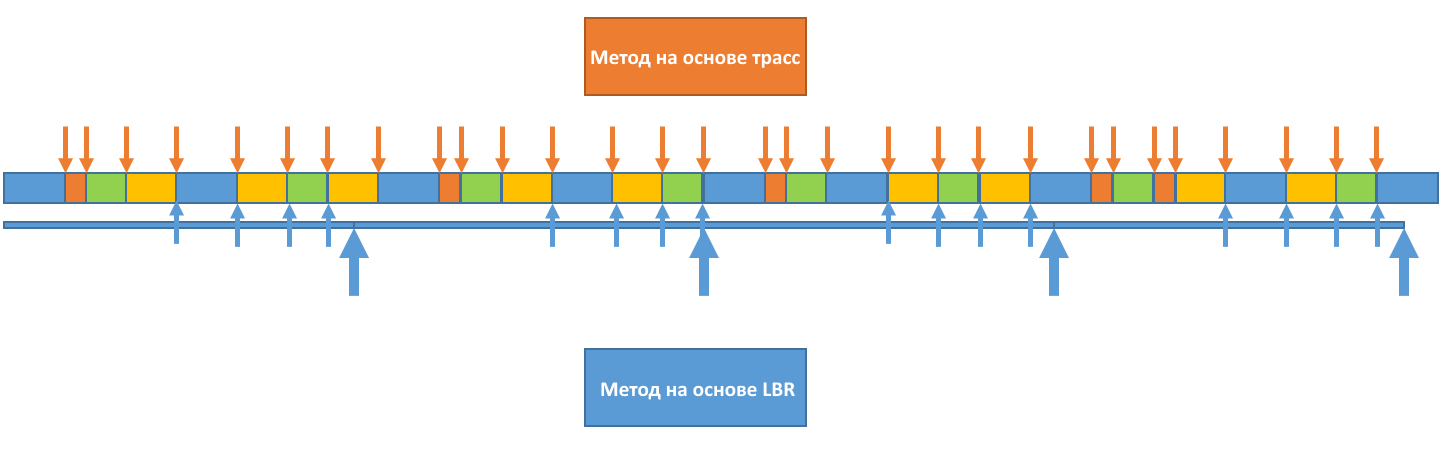
\includegraphics[width=1.0\linewidth]{vs1}
    }
    \caption{Сравнение методов сбора профильной информации}\label{fig:LBRvsTRace}
\end{figure}

Разные методы сбора профильной информации приводят к генерации различных профилей. В данном примере LBR не будет учитывать горячий переход между синим и красным базовыми блоками, что приведёт к не оптимальным преобразованиям бинарного файла (рисунок \cref{fig:LBRvsTraceRes}).
 
\begin{figure}[ht]
    \centerfloat{
        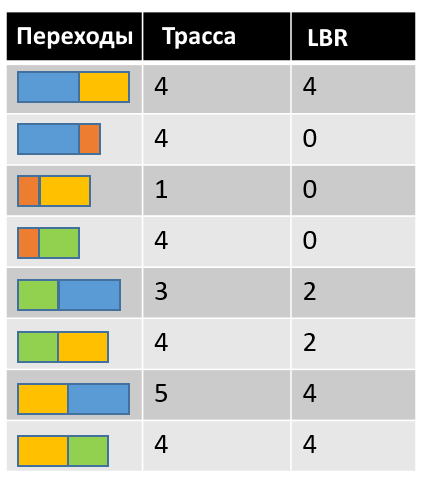
\includegraphics[width=0.5\linewidth]{vs2}
    }
    \caption{Профили, полученные с помощью трассы и LBR}\label{fig:LBRvsTraceRes}
\end{figure}

	Если рассматривать данный пример при большем времени исполнения, то статистически профили будут получены одинаковые. При этом если добавить задержку на обращение в память, то более горячими базовыми блоками станут те, на которых происходило ожидание чтение/записи данных и N-1 предыдущих базовых блоков, где N – размер буфера LBR. Так как основная цель данной оптимизации является улучшение работы инструкционного кэша, то возникает искажение профиля, приводящая к понижению средней температуры L1i.

Метод сбора профильной информации с использованием трассы исполнения был проверен на приложениях, собранных под архитектуру ARM. Для аналогичных программ под x86 собранные с помощью LBR профили коррелируют с полученными выше, что позволяет использовать динамическую бинарную инструментацию с последующим анализом переходов для использования с BOLT.

Профиль, сгенерированный с помощью трасс, для демонстрационного примера изображен в таблице \cref{tab:ARMTrace}.
\begin{table} [h]% Пример записи таблицы с номером, но без отображаемого наименования
    \centering
    \begin{threeparttable}% выравнивание подписи по границам таблицы
        \caption{Профиль демонстрационного примера на ARM архитектуре, собранный с трассы исполнения приложения}%
        \label{tab:ARMTrace}%
        \begin{SingleSpace}
            \begin{tabular}{| c | c | c | c | c | c | c | c |}
                \hline
				1& main& 150& 0& [unknown]& 0& 1& 1 \\ \hline
				0& [unknown]& 0& 1& main& 13c& 1& 1 \\ \hline
				1& falseFunc& 6c& 1& main& 104& 6309097& 6309097 \\ \hline
				1& falseFunc& 60& 1& falseFunc& 28& 0& 28391358 \\ \hline
				1& falseFunc& 34& 1& falseFunc& 64& 6256725& 6309097 \\ \hline
				1& falseFunc& 34& 1& falseFunc& 38& 0& 28391358 \\ \hline
				1& falseFunc& 24& 1& falseFunc& 28& 0& 6309097 \\ \hline
				1& main& 100& 1& falseFunc& 0& 0& 6309097 \\ \hline
				1& main& 120& 1& main& 68& 0& 9999999 \\ \hline
				1& main& dc& 1& main& 110& 0& 3690902 \\ \hline
				1& trueFunc& 6c& 1& main& d0& 3690902& 3690902 \\ \hline
				1& main& cc& 1& trueFunc& 0& 0& 3690902 \\ \hline
				1& condition& 78& 1& main& a8& 9999999& 9999999 \\ \hline
				1& main& a4& 1& condition& 0& 0& 9999999 \\ \hline
				0& [unknown]& 0& 1& main& 94& 9999999& 9999999 \\ \hline
				1& main& 78& 1& main& 124& 75& 1 \\ \hline
				1& main& 78& 1& main& 7c& 0& 9999999 \\ \hline
				1& main& 64& 1& main& 68& 0& 1 \\ \hline
				0& [unknown]& 0& 1& main& 0& 1& 1 \\ \hline
				1& trueFunc& 60& 1& trueFunc& 28& 0& 16608642 \\ \hline
				1& trueFunc& 34& 1& trueFunc& 64& 4429145& 3690902 \\ \hline
				1& trueFunc& 34& 1& trueFunc& 38& 0& 16608642 \\ \hline
				1& trueFunc& 24& 1& trueFunc& 28& 0& 3690902 \\ \hline
				1& \_start& 4& 1& do\_arm64\_start/1& 0& 0& 1 \\ \hline
				0& [unknown]& 0& 1& \_start& 0& 1& 1 \\ \hline
				1& main& a8& 1& main& e0& 2347424& 6309097 \\ \hline
				1& main& a8& 1& main& ac& 0& 3690902 \\ \hline
				0& [unknown]& 0& 1& condition& 3c& 9999999& 9999999 \\ \hline
				1& main& 110& 1& main& 114& 0& 9999999 \\ \hline
				1& main& 10c& 1& main& 110& 0& 6309097 \\ \hline
				1& main& 20& 1& main& 54& 0& 1 \\ \hline
            \end{tabular}%
        \end{SingleSpace}
    \end{threeparttable}
\end{table}
	
Точное сравнение профилей невозможно сделать по двум причинам:
\begin{enumerate}[beginpenalty=10000]
  \item Различие в архитектурах и самих бинарных файлов.
  \item Различие методов сбора профильной информации приложения.
\end{enumerate}

Поэтому сравнение производилось по соотношению основных показателей статистики по тем переходам, по которым можно построить соответствие с исходным кодом. Например, 12 строчка демонстрационного кода (рисунок \cref{fig:TestCode}) соответствует инструкции CBZ по адресу 0x98C (Приложение \cref{lst:ARM}, Листинг Б.1) в бинарном файле для ARM архитектуры и инструкции JE по адресу 0x135E (Приложение \cref{lst:X86}, Листинг Б.2) в бинарном файле для x86 архитектуры.

Полученные адреса инструкций необходимо найти в соответствующей профильной информации. Для ARM архитектуры из таблицы \cref{tab:ARMTrace} следует запись \textbf{1 main a8 1 main e0 2347424 6309097} (так как адрес начала функции main 0x8E4), а для x86 архитектуры запись из таблицы \cref{tab:X86LBR} \textbf{1 main 9e 1 main cd 317 730} (так как адрес начала функции main 0x12C0).

Также в профильной информации есть особенность записи для условных переходов. Для каждой такой инструкции будет сгенерировано две записи:
\begin{enumerate}[beginpenalty=10000]
  \item Запись из инструкции перехода в целевой адрес с указанием предсказанных и взятых исполнений.
  \item Запись из инструкции перехода на следующую инструкцию (при не выполнении условия). При этом в информации от предсказателя переходов нет необходимости.
\end{enumerate}

Для выбранного перехода второй тип записи будет следующим: \textbf{1 main a8 1 main ac 0 3690902} для примера на ARM (таблица \cref{tab:ARMTrace}) и \textbf{1 main 9e 1 main a4 0 421} для x86 (таблица \cref{tab:X86LBR}).

Чтобы проверить корректность полученного профиля для ARM, необходимо сравнить соотношение взятых переходов первого типа записи ко второму. Для обеих архитектур оно должно получиться одинаковым в том случае, если функция condition работает идентично на всех случаях. Полученные значения: 0.58 для ARM и 0.57 для x86 показывают корректность полученного профиля.

\begin{figure}[!h]
    \centerfloat{
        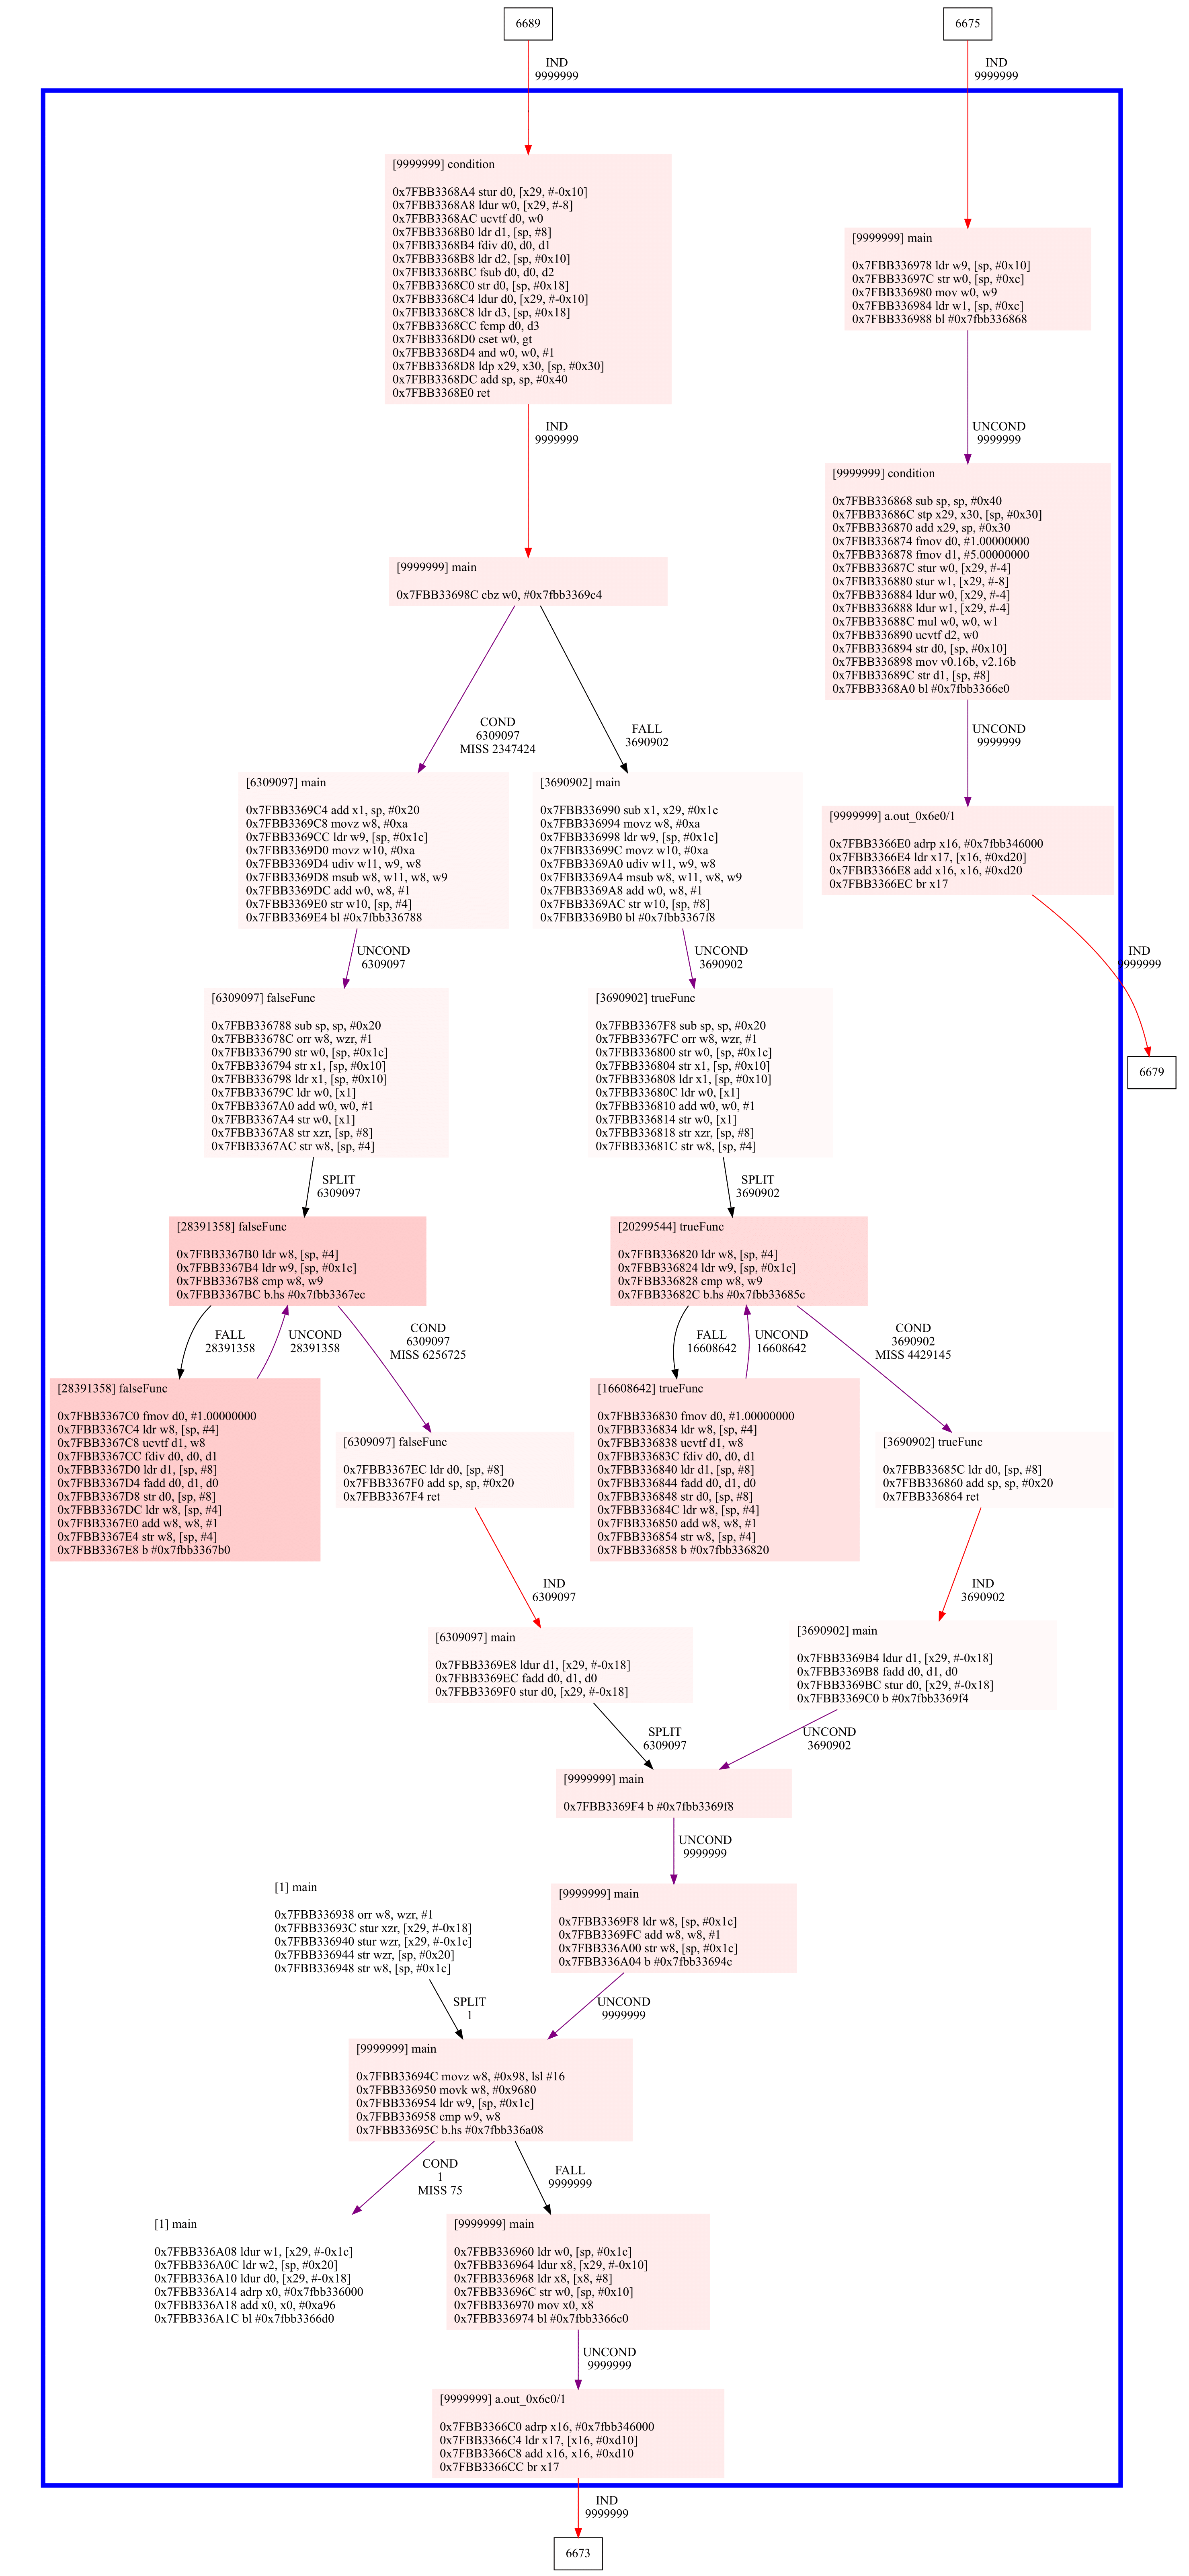
\includegraphics[width=0.6\linewidth]{ARM_graph-1}
    }
    \caption{Граф управления синтетического теста с профильной информацией}\label{fig:DEMOCFG}
\end{figure}

По синтетическому примеру с записанной трассы был собран граф потока управления (рисунок \cref{fig:DEMOCFG}), позволяющий проанализировать работу приложения и часто исполняемые участки кода (более красные линейные участки - чаще исполняемые).

\section{Описание синтетических тестов}\label{sec:ch2/sec5}
Для проверки прироста производительности предложенного метода  сбора профильной информации искусственно были созданы тесты, в которых исполняемый код перемешан с неисполняемым холодным кодом, что приводит к неэффективному использованию инструкционного кэша. Для генерации бинарного файла большого размера (> 10 МБ) применяется рекурсивный вызов шаблонных функций в языке программирования C++. С их помощью компилятор создавал множественные копии функций с разными шаблонными константами, тем самым увеличивая размер кода до нужного значения. Исполняемый код равномерно распределяется по секции, перемежаясь с холодными функциями. 
Примеры синтетических тестов приведены в Приложении \cref{app:A}.

Изначально был сделан тест без стандартной библиотеки для того, чтобы потенциально сложных для бинарного оптимизатора мест было как можно меньше (Приложение \cref{app:A}, Листинг A.1).

В тестовом примере в цикле hot\_repeat раз  производятся рекурсивные вычисления с помощью функций hotFunc<CODE\_SIZE>. Шаблонный параметр выбирается таким, чтобы компилятор сгенерировал бинарный файл большого размера, так как будут созданы экземпляры для всех функций, используемых в программе, с параметрами от CODE\_SIZE до 0 с шагом 1.

\begin{ListingEnv}[h]
    \captiondelim{ } % разделитель идентификатора с номером от наименования
    \caption{Функция main синтетического примера без стандартной библиотеки}\label{lst:hwplain}
    \begin{lstlisting}[language={[ISO]C++}]
    calcFunc<CODE_SIZE>(1);
    for (unsigned int i = 0; i < hot_repeat; i++)
    {
        hotFunc<CODE_SIZE>(1);
    }
    return 0;
    \end{lstlisting}
\end{ListingEnv}%

Для того чтобы генерация всех шаблонов прошла успешно, перед циклом вызывается функция calcFunc<CODE\_SIZE>, заставляющая компилятор создать все экземпляры. Эта функция отвечает за вычисления значений и несёт в себе вычислительную нагрузку данного теста. Она является аналогом демонстрационного приложения с рисунка \cref{fig:TestCode}.

\begin{ListingEnv}[!h]
    \captiondelim{ }
    \caption{Функция calcFunc синтетического примера без стандартной библиотеки}\label{lst:hwbeauty}
    \begin{lstlisting}[language={[ISO]C++}]
template<unsigned int param>
double calcFunc(unsigned int calc_args) 
{
    double res = 0.0;
    unsigned int TRUE = 0, FALSE = 0;
    unsigned int arg = param % 3;
    unsigned int itNumber = calc_args;
    
    if (itNumber == UINT_MAX) {
        calcFunc<param-1>(calc_args);
    }

    for (unsigned int i = 1; i <= itNumber; i++)
    {
        if (condition<param>(i, arg))
        {
            res += trueFunc<param>(i, &TRUE);
        } else {
            res += falseFunc<param>(i, &FALSE);
        }
    }
    return res;
}
    \end{lstlisting}
\end{ListingEnv}%

В теле функции есть вызов самой себя, но с декрементированным шаблонным параметром. Это создаст рекурсивный вызов шаблонных функций до нулевого параметра, так как в коде прописана специализация случая calcFunc<0>. При этом условие написано так, что на входных значения оно выполняться не будет, но код компилятор должен сгенерировать.

После того как один раз были созданы все экземпляры функций calcFunc, condition, trueFunc и falseFunc, размер бинарного файла стал нужного размера. В цикле функции main будет исполняться hotFunc, которая рекурсивно вызывает себя с шагом шаблонного параметра CODE\_STEP. Данный подход помогает чередовать часто используемые функции с не используемыми в бинарном файле.

\begin{ListingEnv}[!h]
    \captiondelim{ }
    \caption{Функция hotFunc синтетического примера без стандартной библиотеки}\label{lst:hwbeauty}
    \begin{lstlisting}[language={[ISO]C++}]
template<unsigned int param>
double hotFunc(unsigned int calc_args)
{
    return calcFunc<param>(calc_args) + hotFunc<param - CODE_STEP>(calc_args);
}
    \end{lstlisting}
\end{ListingEnv}%

Для компиляции примера без использования стандартной библиотеки необходимо написать стартовый файл на ассемблере целевой архитектуры. Примеры стартовых файлов приведены в Приложении \cref{app:A}, Листинг A.2 для ARM архитектуры и Листинг A.3 для архитектуры x86.

Второй тест написан уже с использованием стандартной библиотеки, что позволяет использовать вывод в консоль и проверить корректность вычисляемых значений (Приложение \cref{app:A}, Листинг A.4).

Последний тест написан с дополнением в виде использования исключений и виртуальных функций для проверки работы бинарного оптимизатора BOLT на подобных примерах (Приложение \cref{app:A}, Листинг A.5).

\section{Результаты тестирования}\label{sec:ch2/sec6}
Полученные статистические данные (рисунок \cref{fig:SynRes}) показывают понижение практически до нуля количество промахов по iTLB, увеличение IPC (instruction per clock) на 41\% и уменьшение времени работы на 29\%. Как было сказано выше, для тестирования была выбрана микроархитектура ARM Cortex A76 \cite{vakbib1}.
\begin{figure}[!h]
    \centerfloat{
        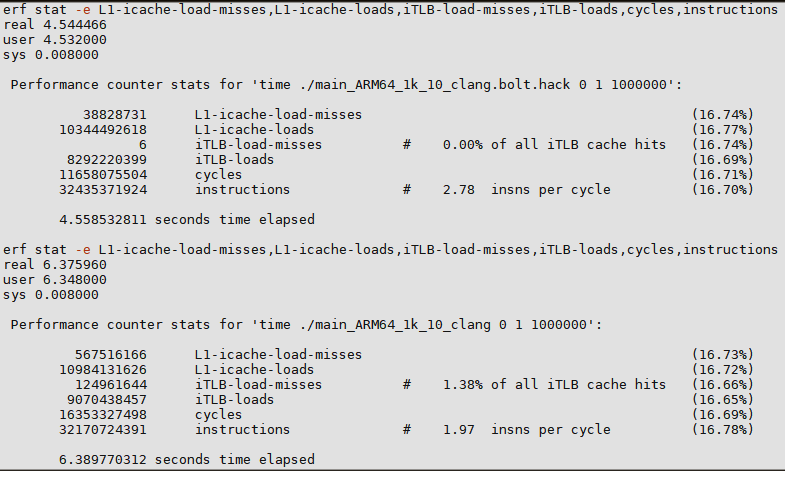
\includegraphics[width=1.0\linewidth]{13}
    }
    \caption{Сравнение результатов запусков оригинального и оптимизированного бинарных файлов синтетического теста}\label{fig:SynRes}
\end{figure}

Данные результаты повторяются на всех синтетических тестах, включая три теста, описанных в предыдущем разделе. На всех оптимизированных тестах отсутствуют промахи по iTLB в случае, когда суммарный размер часто исполняемых линейных участков не превышает размера отображаемого кода iTLB.

\section{Вывод по главе}\label{sec:ch2/sec7}
Во второй главе проводится анализ существующего подхода в бинарном оптимизаторе BOLT, который позволил предложить альтернативный способ получения профильной информации приложения на основе трасс исполнения.

Предлагаемая схема оптимизации бинарного файла на ARM архитектуре была протестирована на синтетических тестах.
\newpage
Также было проведено сравнение подходов на основе аппаратной поддержки с LBR и на основе трасс исполнения. Анализ полученных профилей подтверждает корректность применения предложенного подхода.

Приводимые результаты запусков, которые были оптимизированы на основе профильной информации, собранной из трасс исполнения синтетических тестов, подтверждают возможность использования данного метода.

\clearpage           % Глава 2
\chapter{Улучшения бинарного оптимизатора BOLT}\label{ch:ch3}
Данная глава посвящена вопросам улучшения бинарного оптимизатора BOLT под ARM архитектуру.

В разделе 3.1 рассматривается проблема длинных переходов в бинарной оптимизации. Предлагается метод оптимизации трамплинов, позволяющий уменьшить количество добавляемых для трамплина инструкций и не использовать дополнительный регистр.

В разделе 3.2 обсуждается проблема бинарной оптимизации исполняемых файлов под ARM архитектуру, в которых используются таблицы переходов. Предлагается метод обхода данной проблемы.

В разделе 3.3 предлагается метод верификации оптимизированного бинарного файла. Приводится описание разработанного формата преобразования, позволяющего проверить корректность перекомпоновки кода. Приводятся разработанные правила верификации и разрешенные преобразования. Показаны результаты верификации и найденные ошибки.

В разделе 3.4 описываются результаты тестирования синтетических тестов и общих наборов тестов после оптимизации модифицированным бинарным транслятором BOLT.

\section{Оптимизация длинных переходов}\label{sec:ch3/sect1}
Помимо отсутствия LBR, ARM архитектура накладывает дополнительные ограничения на перемещение горячих базовых блоков. Перекомпоновка кода проще реализуется на CISC архитектуре за счёт возможности добавления длинных прыжков одной инструкцией. На RISC архитектурах количество битов смещения в инструкциях переходов меньше, что приводит к ограничению диапазона возможного перемещения. Также инструкция загрузки в регистр адреса, который зависит от счетчика инструкций, на ARM архитектуре ограничена 20 битами, выделенными на смещение, и накладывает возможный диапазон перемещения ± 1 мегабайт (рисунок \cref{fig:CmpPcRel}). Все инструкции, зависящие от адреса инструкции (переходы, загрузка адреса, загрузка по регистру/смещению) после оптимизации необходимо проверить на возможность записи нового смещения в отведенные для этого биты \cite{Blem2013} \cite{confbib1}.

\begin{figure}[ht]
    \centerfloat{
        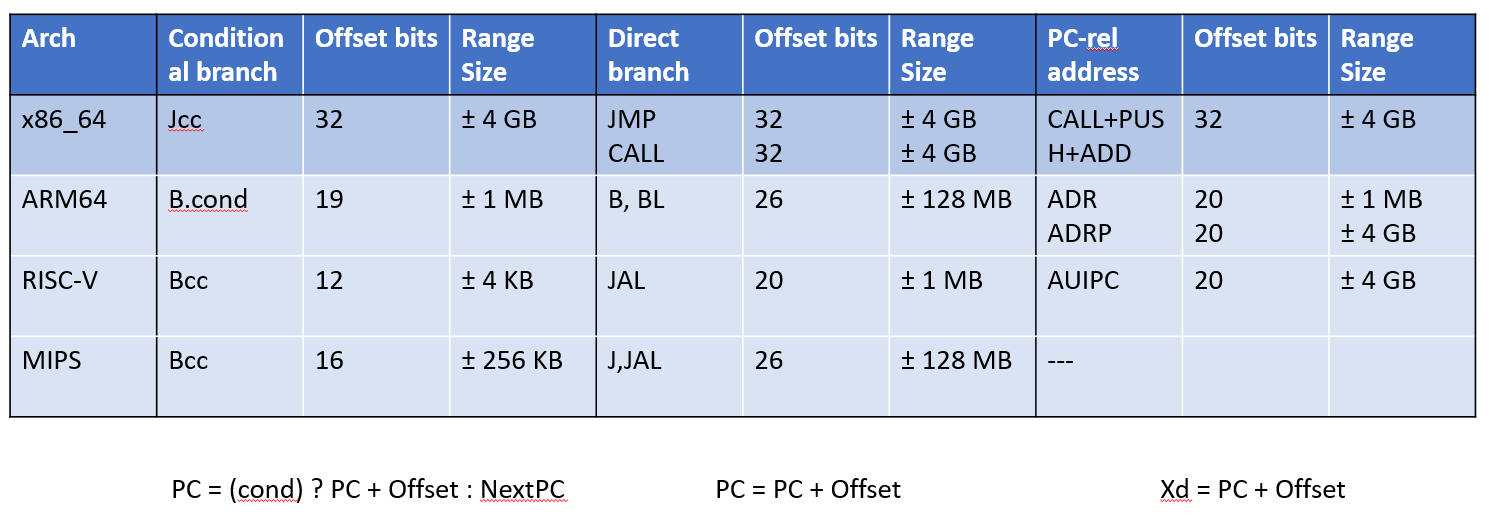
\includegraphics[width=1.0\linewidth]{pcrel}
    }
    \caption{Сравнение инструкций, зависящих от счетчика инструкций}\label{fig:CmpPcRel}
\end{figure}

Таким образом, при перемещении горячего кода, который ссылается на холодный участок (черная стрелка), происходит переполнение значения смещения и оптимизация становится некорректной (рисунок \cref{fig:HotMove}).

\begin{figure}[ht]
    \centerfloat{
        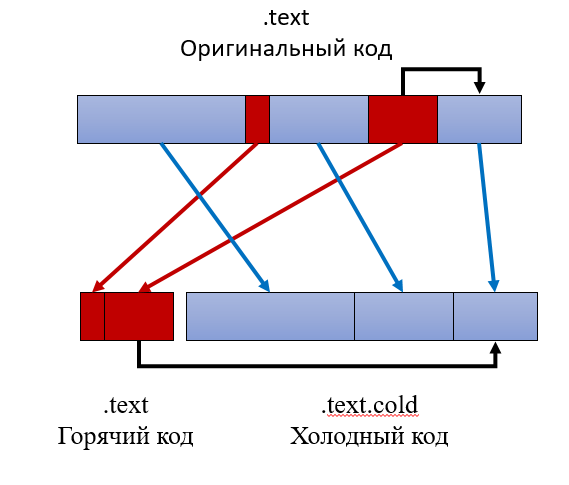
\includegraphics[width=0.8\linewidth]{11}
    }
    \caption{Пример перекомпоновки горячего кода}\label{fig:HotMove}
\end{figure}

Для решения данной проблемы необходимо добавить трамплин – дополнительный код, позволяющий генерировать произвольный адрес и произвести переход либо загрузку по данному значению (рисунок \cref{fig:Tramp}). Подобное решение будет увеличивать размер кода, что приведёт к понижению производительности, при этом диапазон перемещаемого кода будет увеличен. Также необходимо наличие свободного регистра, в который будет записываться данный адрес.

\begin{figure}[ht]
    \centerfloat{
        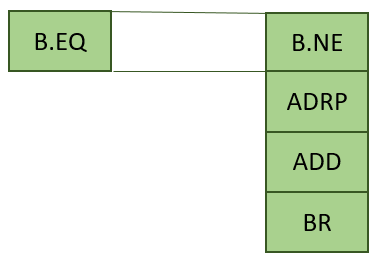
\includegraphics[width=0.5\linewidth]{opt3}
    }
    \caption{Генерация трамплина для инструкции условного перехода}\label{fig:Tramp}
\end{figure}

Альтернативный подход – генерация таблицы трамплинов рядом с горячим кодом. Таким образом, поток управления будет проходить через неё в случае прыжка из горячего кода в холодный. Данный подход решит проблему инструкций переходов без увеличения размера горячего кода. В обратном направлении можно вставлять трамплины прямо в холодный код, так как его размер не сильно повлияет на изменение производительности.

Для условных переходов можно написать маленькие трамплины размером в одну инструкцию с помощью добавления одного безусловного перехода, если смещение занимает больше 19, но меньше 26 бит (рисунок \cref{fig:CmpBranch}).

\begin{figure}[ht]
    \centerfloat{
        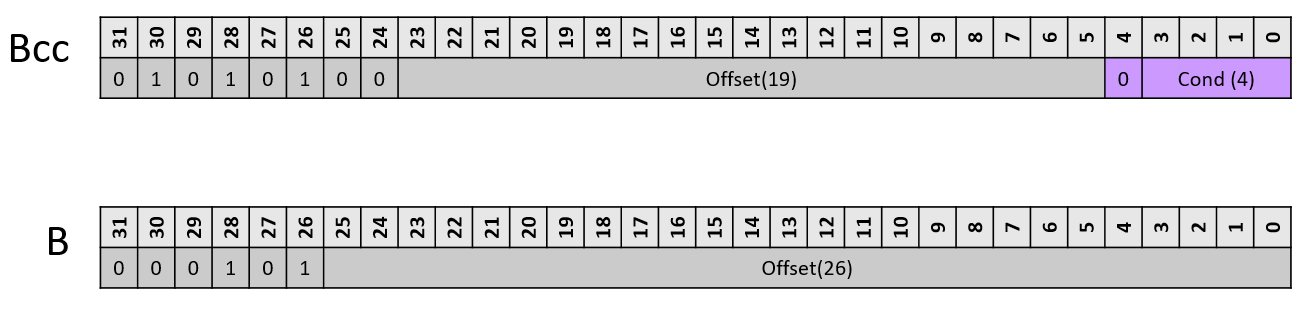
\includegraphics[width=1.0\linewidth]{opt1}
    }
    \caption{Сравнение условного и безусловного перехода}\label{fig:CmpBranch}
\end{figure}

\begin{figure}[ht]
    \centerfloat{
        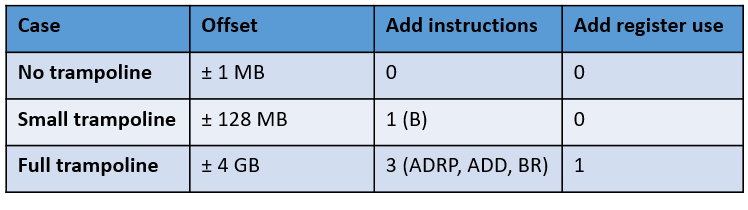
\includegraphics[width=1.0\linewidth]{opt4}
    }
    \caption{Сравнение трамплинов}\label{fig:CmpTramp}
\end{figure}

В этом случае необходимо инвертировать условие инструкции, а метку для прыжка поставить через одну инструкцию прямого перехода, вставленную оптимизатором непосредственно после условного перехода (рисунок \cref{fig:CmpTramp}). В результате региона перемещения увеличивается в 128 раз за счёт отличий в кодировке Bcc и B, а увеличение кода произошло всего на 1 инструкцию (рисунок \cref{fig:ExTramp}).
 
\begin{figure}[ht]
    \centerfloat{
        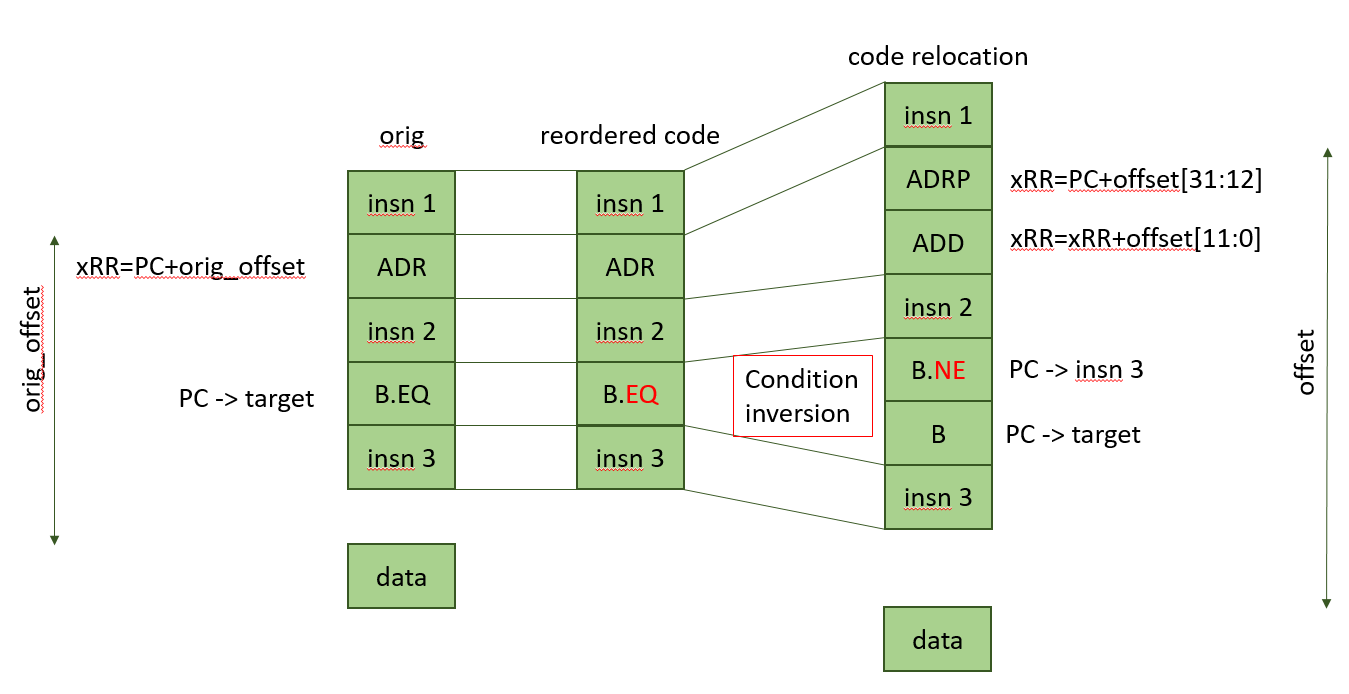
\includegraphics[width=1.0\linewidth]{opt2}
    }
    \caption{Схема добавления трамплинов для ADR (сверху) и Bcc (снизу) инструкций}\label{fig:ExTramp}
\end{figure}

В верхней части рисунка \cref{fig:ExTramp} изображено решение для ADR инструкции. Если увеличение смещения больше возможного, инструкция заменяется на пару ADRP+ADD, это увеличивает возможный регион перемещений с 1 мегабайт до 4 гигабайт и покрывает все необходимые расстояния.
И последний тип инструкций, зависящий от адреса команды - загрузки по регистру/смещению. В простейшем варианте проблемы с большим смещением решается добавлением одной инструкции ADR.
Данные подходы позволили оптимизировать большинство приложений, при добавлении лишь одной дополнительной инструкции на каждый случай.

\section{Исправление преобразования таблиц переходов}\label{sec:ch3/sect2}

Помимо проблем с недостаточным количеством битов в инструкциях на ARM архитектуре, была найдена проблема с таблицей переходов (jump table). При перемещении кода конкретного варианта конструкции switch-case необходимо модифицировать запись в таблице, используемую в косвенном переходе. Оптимизатор узнает адрес записи из релокационной информации, которая для некоторых случаев кода ARM архитектуры не будет корректной. Это происходит по причине несоответствия адреса, от которого вычисляется целевой адрес для прыжка при исполнении и генерации релокационной информации.

Рассмотрим пример, приведенный на рисунке \cref{fig:SC1}. Конструкция switch-case реализуется через трамплин на код конкретного case-кода, расположенного по адресу \textbf{CASE2\_ADR}. За 3 инструкции (ADD, LDR, ADD) происходит вычисление этого адреса в регистре X2, а четвертой инструкцией BR - перемещение на код case2.

Для вычисления этого адреса предварительно были подготовлены следующие значения: регистр X0 - номер рассматриваемого case, регистр X1 - адрес начала таблицы переходов, память по адресу \textbf{JTR2\_ADR} - смещение относительно данного адреса до \textbf{<case2 code>} \textbf{JTR2\_VAL}.

Вычисление регистра X2 для перехода по нему происходит в три этапа:
\begin{enumerate}[beginpenalty=10000]
  \item Вычисление \textbf{JTR2\_ADR} в регистре X3.
  \item Загрузка значения \textbf{JTR2\_VAL} в регистр X2.
  \item Вычисление \textbf{CASE2\_ADR} в регистре X2.
\end{enumerate}


\begin{figure}[!h]
    \centerfloat{
        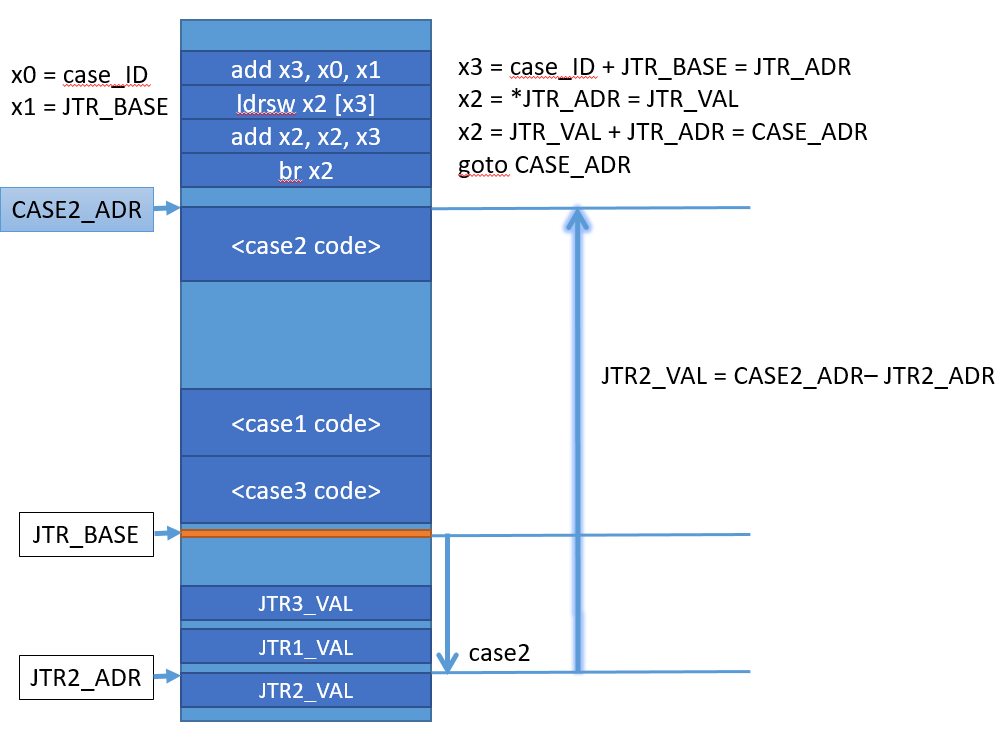
\includegraphics[width=1.0\linewidth]{jt2}
    }
    \caption{Пример ассемблерного кода для switch-case случая}\label{fig:SC1}
\end{figure}

В бинарном файле есть специальная релокационная секция, где записана вся информация об инструкциях и данных, зависящих от счетчика инструкций (PC-relative). В данном примере таким значением является  \textbf{JTR2\_VAL}. Для него записываются три поля релокационной записи: адрес, тип (PREL32 -- PC Relative 32 bit) и в нём хранящееся значение. Для \textbf{JTR2\_VAL} запись приведена на рисунке \cref{fig:Rel1}.

\begin{figure}[!h]
    \centerfloat{
        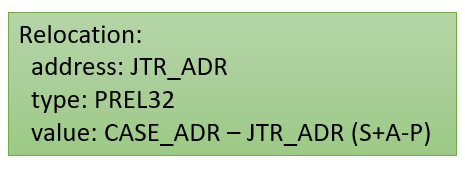
\includegraphics[width=0.6\linewidth]{jt_1}
    }
    \caption{Заполненная структура релокационной записи для перехода по значению регистра}\label{fig:Rel1}
\end{figure}

Релокационная информация необходима для того, чтобы после перестановки кода в бинарном файле можно было переписать все значения, зависящие от счетчика инструкций. На рисунке \cref{fig:SC2} приведен пример перемещения \textbf{<case2 code>}, в результате которого \textbf{JTR2\_VAL} будет переписан, чтобы указывать на новое местоположение кода (зеленые поля).

\begin{figure}[!h]
    \centerfloat{
        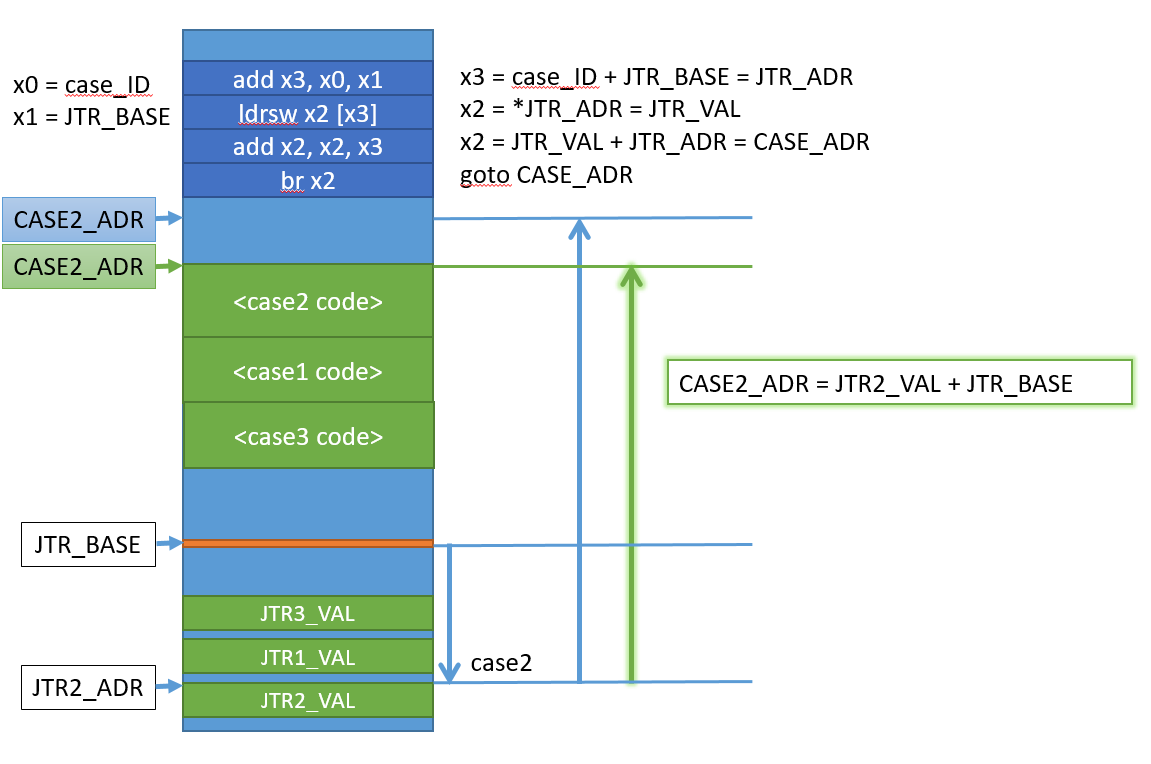
\includegraphics[width=1.0\linewidth]{jt3}
    }
    \caption{Преобразование смещений при перекомпоновке кода}\label{fig:SC2}
\end{figure}

На ARM архитектуре возможно произвести оптимизацию данного примера, уменьшив на одну инструкцию процесс вычисления адреса \textbf{CASE2\_ADR} и освободив один регистр (рисунок \cref{fig:SC3}). Для этого необходимо хранить в таблице переходов смещения не между кодом case и записью в таблице переходов, а между кодом case и началом таблицы перехода. В этом случае второй этап подготовки адреса \textbf{CASE2\_ADR} будет использовать инструкцию LDR, которая будет загружать данные по результату сложения регистров X0 и X1. Тогда первое сложение тогда будет не нужно, и освободится регистр X3, в который до этого записывалось значение \textbf{JTR2\_ADR}.

\begin{figure}[!h]
    \centerfloat{
        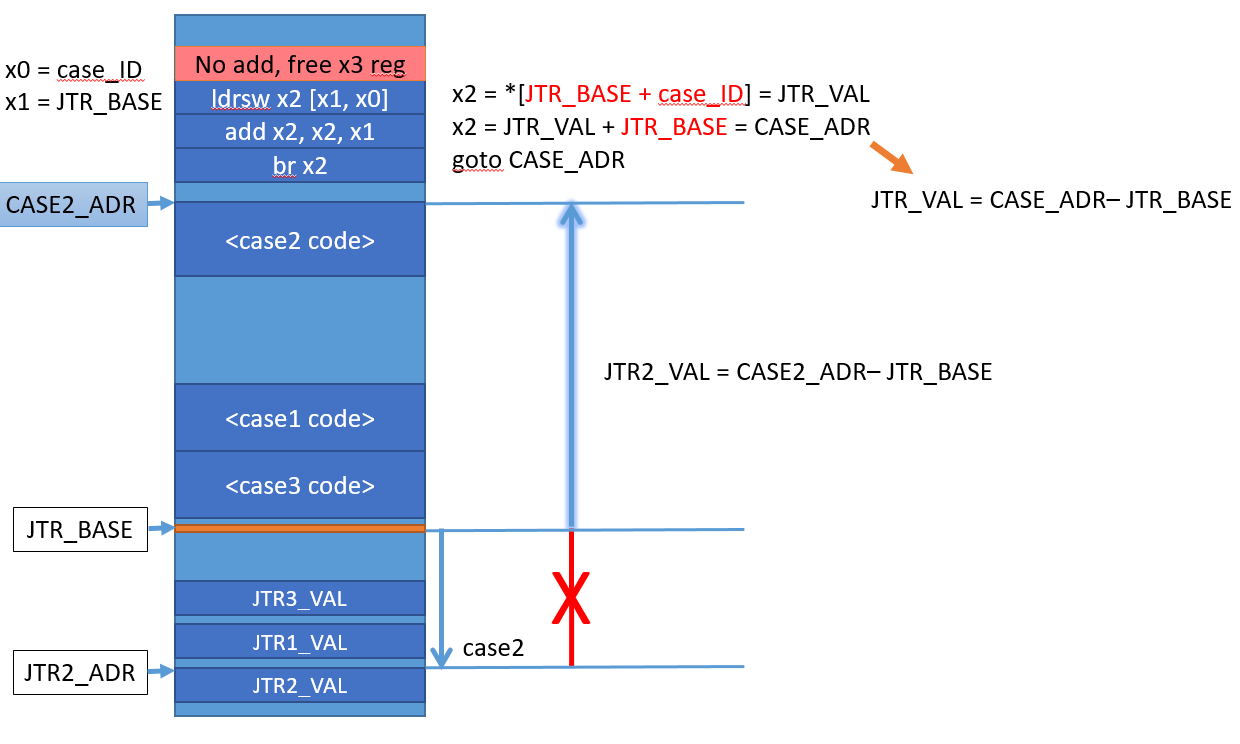
\includegraphics[width=1.0\linewidth]{jt4}
    }
    \caption{Оптимизированный вариант ассемблерного кода для switch-case случая}\label{fig:SC3}
\end{figure}

При данной оптимизации запись в релокационной секции станет не корректной, так как теперь записанный адрес \textbf{JTR2\_ADR} не соответствует базе, от которой отсчитывается  смещение до \textbf{<case2 code>} (рисунок \cref{fig:Rel2}).

\begin{figure}[!h]
    \centerfloat{
        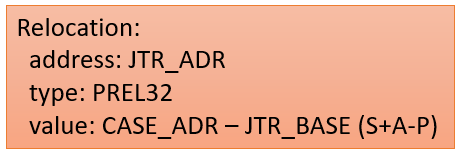
\includegraphics[width=0.6\linewidth]{jt_2}
    }
    \caption{Оптимизированный вариант структуры релокационной записи для перехода по значению регистра}\label{fig:Rel2}
\end{figure}

В данном случае бинарный оптимизатор, прочитав релокационную секцию, будет воспринимать смещение не относительно начала таблицы переходов, а относительно записи в таблице (рисунок \cref{fig:SC4}), и произойдёт смещение на значение \textbf{case\_ID}. То есть релокационная запись указывает на какой-то случайный код \textbf{<some code>} по адресу \textbf{CASE2\_REL}.

\begin{figure}[!h]
    \centerfloat{
        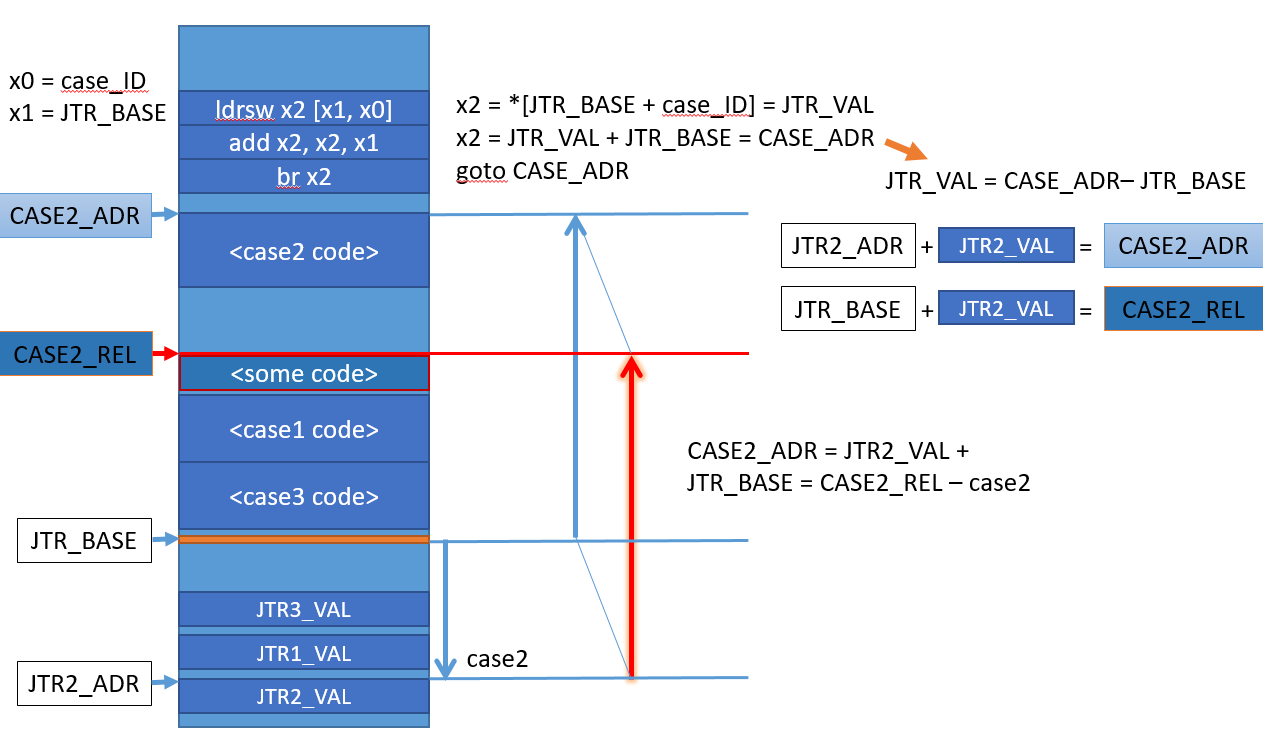
\includegraphics[width=0.8\linewidth]{jt5}
    }
    \caption{Ошибочный расчет целевого адреса бинарным оптимизатором}\label{fig:SC4}
\end{figure}

Когда будет происходить перекомпоновка кода, бинарным оптимизатором будет отслеживаться неверный код, из-за чего таблица переходов будет модифицирована некорректно, если \textbf{<some code>} сместится относительно \textbf{<case2 code>} (рисунок \cref{fig:SC5}).

\begin{figure}[!h]
    \centerfloat{
        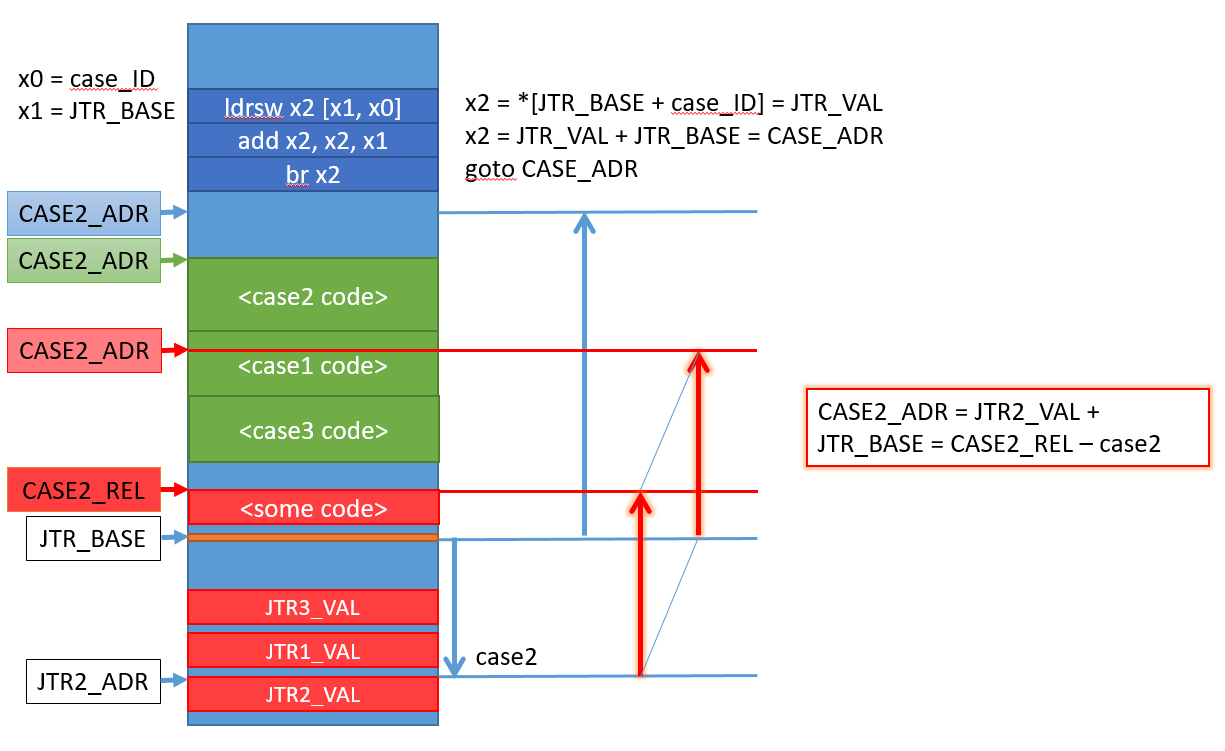
\includegraphics[width=1.0\linewidth]{jt6}
    }
    \caption{Преобразование смещений при перекомпоновке оптимизированного кода}\label{fig:SC5}
\end{figure}

Данная проблема была найдена при оптимизации бинарного файла набора тестов GeekBench (рисунок \cref{fig:SCEx1}). Оптимизация обработки switch-case случая компилятором привела к некорректной релокационной записи и ошибочной модификации записи таблицы перехода (рисунок \cref{fig:SCEx2}).

\begin{figure}[!h]
    \centerfloat{
        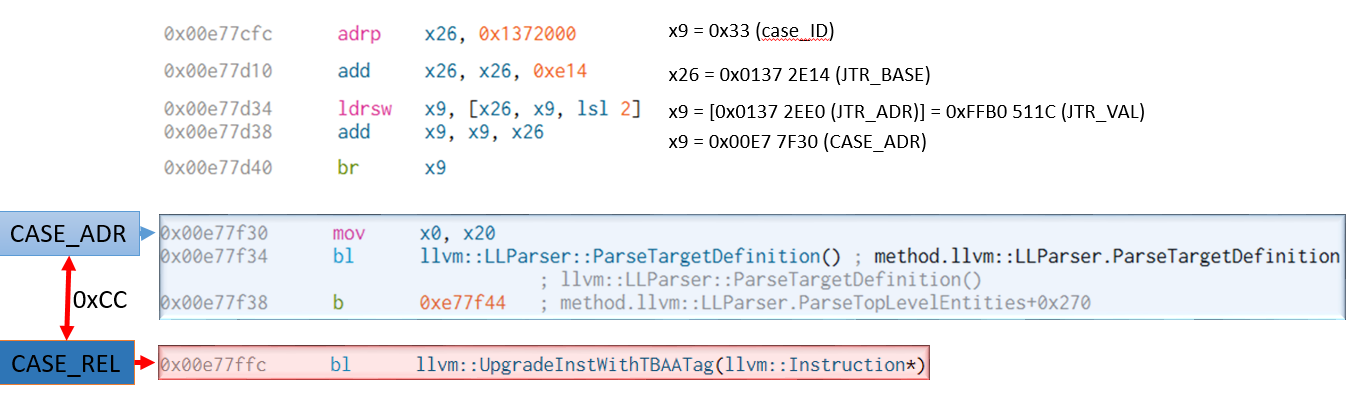
\includegraphics[width=1.0\linewidth]{jt7}
    }
    \caption{Пример кода с переходом по значению регистра (тестовый набор GeekBench)}\label{fig:SCEx1}
\end{figure}

\begin{figure}[!h]
    \centerfloat{
        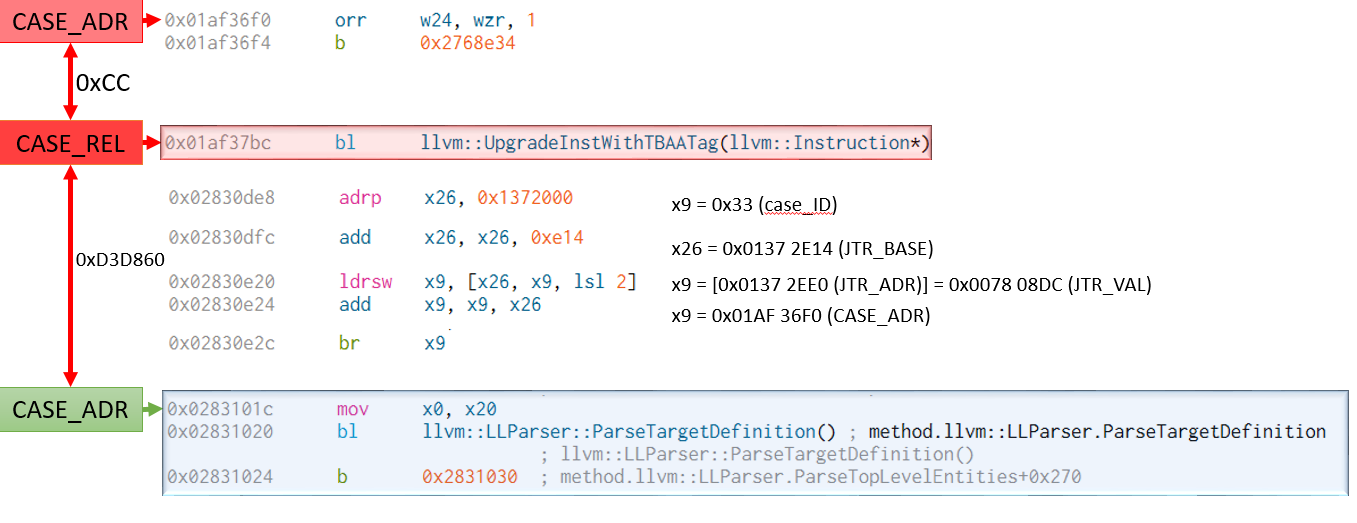
\includegraphics[width=1.0\linewidth]{jt8}
    }
    \caption{Пример кода с переходом по значению регистра после перекомпоновки(тестовый набор GeekBench)}\label{fig:SCEx2}
\end{figure}

Данная проблема была решена переиспользованием оригинального участка кода с данным косвенным переходом. То есть необходимо сохранить копию оригинальной секции .bolt.org.text, так как вычислить из данных релокационной записи адрес начала таблицы переходов в общем случае невозможно.

\section{Верификация бинарной оптимизации}\label{sec:ch3/sect3}
В результате работы бинарного оптимизатора BOLT генерируется новый исполняемый файл, в котором добавлены новые оптимизированные секции. Этот файл показывает лучшие характеристики производительности в сравнении с оригинальным, но помимо перестановки кода есть возможность провести другие оптимизации как общие, так и микроархитектурные. BOLT позволяет дописывать дополнительные проходы, соответствующие новым оптимизациям, но усложнение транслятора ведёт к более сложной отладке возможных проблем и верификации полученного оптимизированного исполняемого файла.

Для решения данной задачи было предложено разработать специальный формат, описывающий преобразования исполняемого файла в оптимизированный, так называемый remap-файл (рисунок \cref{fig:Remap}). В нём записывается информация о всех совершенных перестановках кода и дополнительная информация, обозначающая инструкции, подвергнутые преобразованиям в процессе перекомпоновки (PC-relative инструкции).


\begin{figure}[!h]
    \centerfloat{
        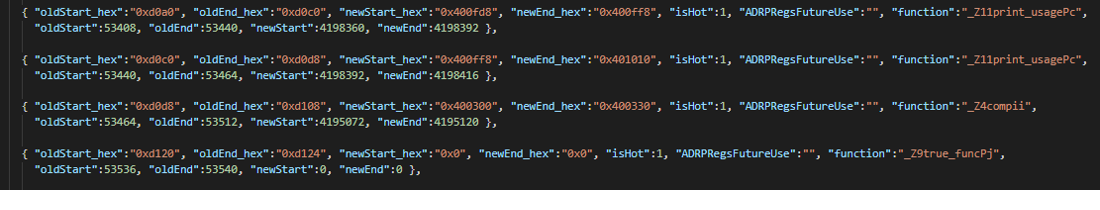
\includegraphics[width=1.0\linewidth]{v1}
    }
    \caption{Пример файла преобразований бинарного файла}\label{fig:Remap}
\end{figure}

Каждая запись относится к одному линейному участку и включает в себя новые и старые начальные и конечные адреса в бинарном файле. Соответствующие начальный и конечный адреса могут совпадать, указывая на пустой блок. Это возможно, если оптимизатор удаляет линейный участок или добавляет новый. Атрибуты с суффиксом <<\_hex>> - это строки с шестнадцатеричным представлением значений в соответствующих атрибутах без суффикса, которые применяются для отладки. <<isHot>> равен 1, если линейный участок часто используемый и был перемещен в секцию горячего кода.

\begin{figure}[!h]
    \centerfloat{
        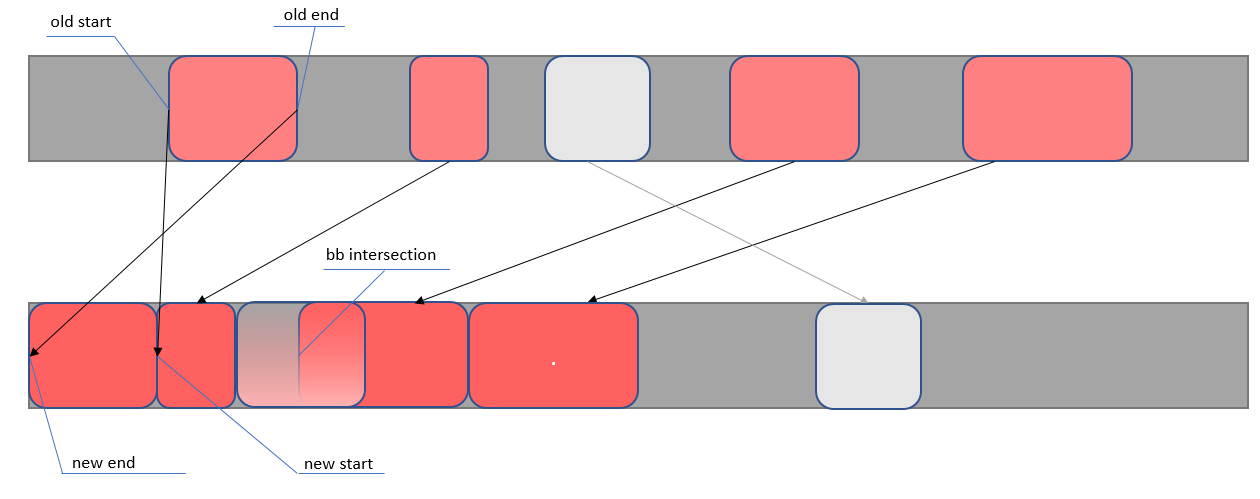
\includegraphics[width=1.0\linewidth]{v2}
    }
    \caption{Схема верификации бинарного файла}\label{fig:Verif}
\end{figure}

В рамках данной работы в BOLT был добавлен проход, генерирующий remap-файл, а также написан статический анализатор, сравнивающий оригинальный и оптимизированный исполняемые файлы по данному remap-файлу (рисунок \cref{{fig:Verif}}). Реализованы следующие проверки:

\begin{enumerate}[beginpenalty=10000]
  \item Проверка корректности оптимизированных линейных участков кода.
  \item Проверка корректности создания теневых точек.
  \item Сравнение инструкций оптимизированных и исходный линейных участков.
\end{enumerate}	

\begin{figure}[!h]
    \centerfloat{
        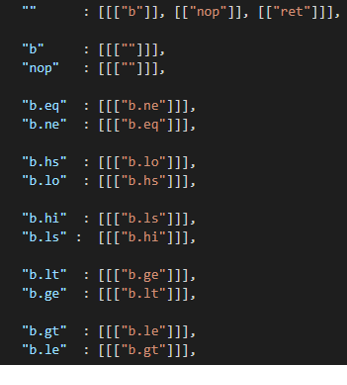
\includegraphics[width=0.6\linewidth]{v3}
    }
    \caption{Пример файла разрешенных преобразований}\label{fig:Access}
\end{figure}

Последний тип проверки использует файл разрешенных преобразований, где описывается преобразования линейного участка (рисунок \cref{fig:Access}).

\begin{figure}[!h]
    \centerfloat{
        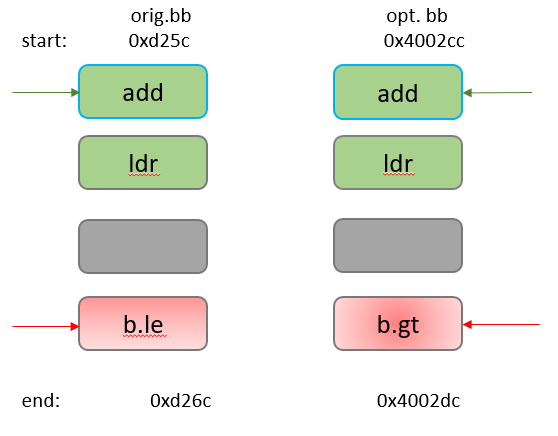
\includegraphics[width=0.6\linewidth]{v4}
    }
    \caption{Проверка линейного участка без изменения количества инструкций}\label{fig:VerifEx1}
\end{figure}

Проверка запускает рекурсивный анализ преобразования линейного участка, последовательно набирая разрешенные преобразования до тех пор, пока линейные участки не совпадут (рисунки \cref{fig:VerifEx1} и  \cref{fig:VerifEx2}).

\begin{figure}[!h]
    \centerfloat{
        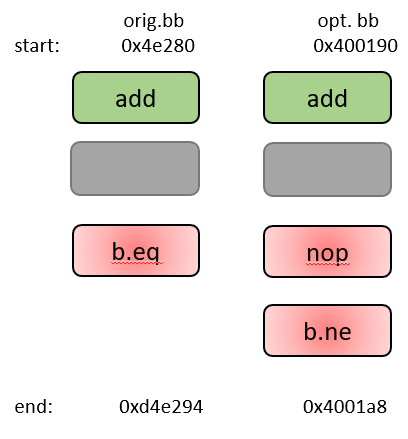
\includegraphics[width=0.5\linewidth]{v5}
    }
    \caption{Проверка линейного участка с измененным количества инструкций}\label{fig:VerifEx2}
\end{figure}

В результате проделанной работы была обеспечена статическая верификация оптимизированных BOLT-ом приложений, что обеспечило выявление ошибок оптимизатора на наборах тестов SPEC CPU 2017 и GeekBench.

\section{Результаты тестирования модифицированного оптимизатора}\label{sec:ch3/sect4}
Реализованный метод генерации профиля и модифицированная версия BOLT для ARM архитектуры были протестированы на описанных выше синтетических тестах.

Для проверки оптимизации на реальном приложении был выбран набор тестов производительности GeekBench. Среди всего набора был выбран тест с наибольшим числом iTLB и L1I промахов – Clang. При компиляции набора тестов были использован флаг <<-O2>>, который соответствует оптимизациям при стандартной сборке приложений \cite{vakbib1}.

\begin{figure}[!h]
    \centerfloat{
        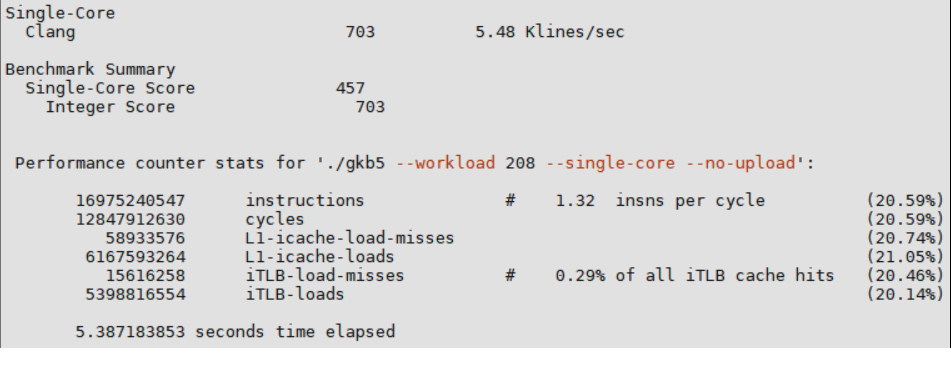
\includegraphics[width=1.0\linewidth]{14}
    }
    \caption{Результаты исполнения оригинального Clang теста}\label{fig:ClangRes1}
\end{figure}

По результатам тестов был получен прирост в показателях теста на 10\%, уменьшение iTLB и L1I промахов на 32\% и 38\% соответственно, что является показателем увеличения средней температуры кода (рисунки \cref{fig:ClangRes2} и \cref{fig:ClangRes2}). При этом остальные тесты из набора GeekBench либо не улучшили производительность, либо ухудшили её.

\begin{figure}[!h]
    \centerfloat{
        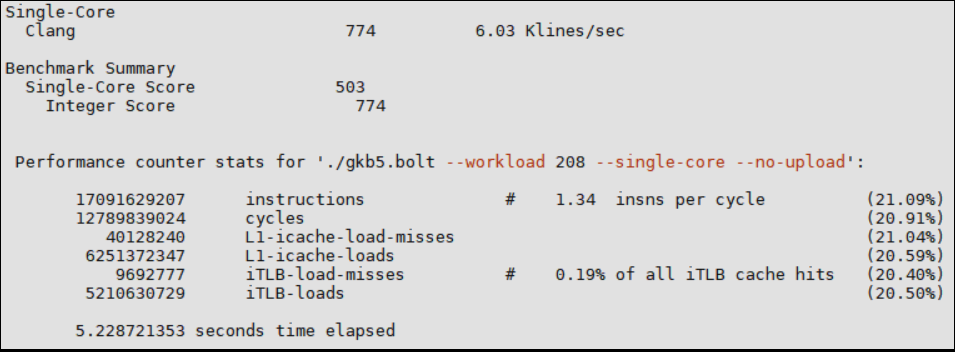
\includegraphics[width=1.0\linewidth]{15}
    }
    \caption{Результаты исполнения оптимизированного Clang теста}\label{fig:ClangRes2}
\end{figure}

Регрессии возникают из-за стандартной проблемы оптимизации на основе профильной информации. Когда исполнение приложения отклоняется от использованного для оптимизации, начинается использование не оптимизированного кода. В случае с BOLT происходит уход исполнения в холодную секцию кода, и средняя температура L1I понижается, приводя к понижению производительности. 

Для решения данной проблемы был реализован режим обработки нескольких трасс одновременно, что исключило регрессии на остальных тестах, а в некоторых случаях и увеличило производительность. Данный режим является аналогом приложения для объединения нескольких профилей, предоставляемого вместе с BOLT.


\section{Вывод по главе}\label{sec:ch3/sect5}
В третьей главе были исследованы существующие проблемы бинарного оптимизатора BOLT, не позволяющие полноценно оптимизировать приложения под ARM архитектуру. В результате проделанной работы удалось реализовать альтернативный способ сбора информации с использованием динамической бинарной инструментации. Исправлены возникающие для данной архитектуры проблемы, связанные с особенностью кодировки команд. Добавлена верификация оптимизированного бинарного файла. Подход протестирован на синтетических тестах и наборе тестов производительности GeekBench и показал ожидаемые результаты.

\clearpage
           % Глава 3
\chapter{Бинарные оптимизации на основе трасс исполнения}\label{ch:ch4}

В этой главе приведено описание бинарных оптимизаций на основе трасс исполнения приложения.

В разделе 4.1 описываются проблемы оптимизаций с профильной информацией. Приводится пример приложения, когда от выбранного сценария зависит, будет получен прирост, или регрессия производительности на приложении.

В разделе 4.2 рассматривается дополнительная информация, которую возможно извлечь из трассы исполнения и применить для последующей бинарной оптимизации приложения.

В разделе 4.3 приводится описание мультипрофильного анализа трасс исполнения приложения. Вводятся основные необходимые термины для данного анализа: интервалы инструкций, фазы исполнения и мультипрофиль.

В разделе 4.4 описывается бинарная оптимизация - дублирование кода на основе мультипрофиля. Рассматриваются основные случаи применимости данной оптимизации.

В разделе 4.5 приводятся результаты запусков тестов, оптимизированных с помощью дублирования кода на основе мультипрофиля.

\section{Проблемы оптимизации с профильной информацией}\label{sec:ch4/sect1}
Профилирование программы – это сбор характеристик работы программы. При работе оптимизатора BOLT необходимы значения счетчика команд и последние взятые переходы с информацией от предсказателя переходов. Во время сбора характеристик программа исполняется по определенному сценарию: конкретные входные данные, параметры окружения, контекст и т.д. Полученная профильная информация будет показывать характеристики этого выбранного сценария.

После оптимизации приложения с данным профилем запуск по данному сценарию будет показывать прирост производительности, но при проверке производительности с другими входными параметрами на данном приложении такого же прироста производительности получить не удастся (вероятно будет происходить регрессия) \cite{Valiante2021}.

Рассмотрим демонстрационное приложение (рисунок \cref{fig:TestCode}), которое может иметь два сценария исполнения.

После сбора профилировочной информации и прохождений оптимизаций BOLT расположит часто использованные линейные участки в секции кода .text, остальные будут размещены в секции кода .text.cold (рисунок \cref{fig:CFGProfile1}).
 
\begin{figure}[!h]
    \centerfloat{
        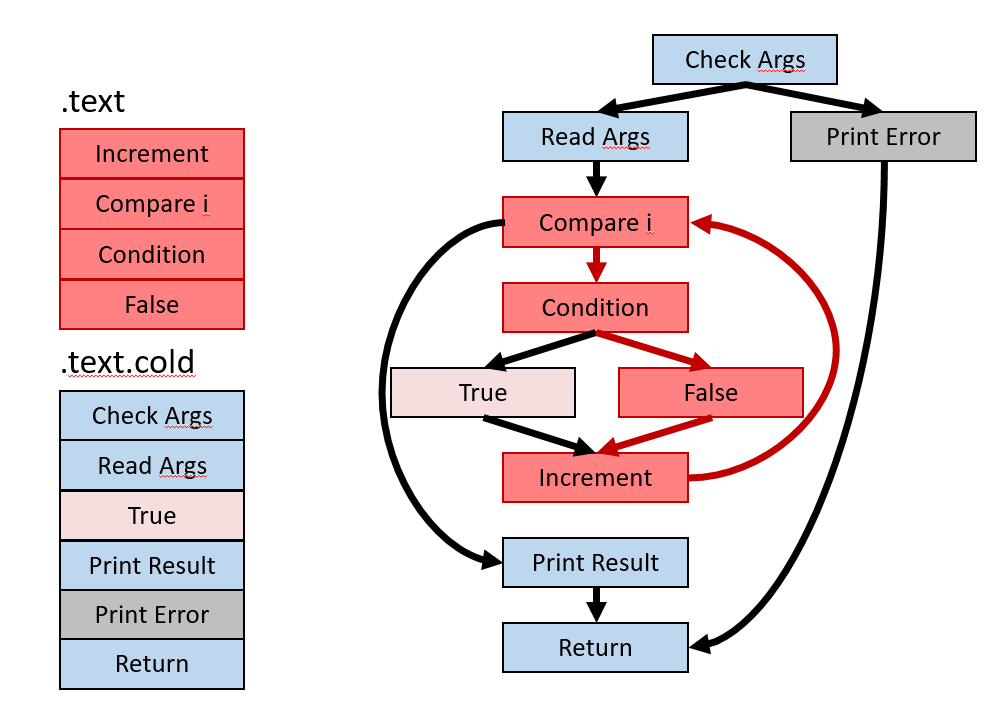
\includegraphics[width=0.8\linewidth]{_3}
    }
    \caption{Граф потока управления с профилем}\label{fig:CFGProfile1}
\end{figure}
Для собранного профиля приложение стало более производительным за счёт расположения всего горячего кода в одном месте. Однако, если исполнение пойдет по другому пути, то производительность понизится из-за перехода в горячий линейный участок «True», расположенный в другой секции (рисунок \cref{fig:CFGProfile2}).

\begin{figure}[!h]
    \centerfloat{
        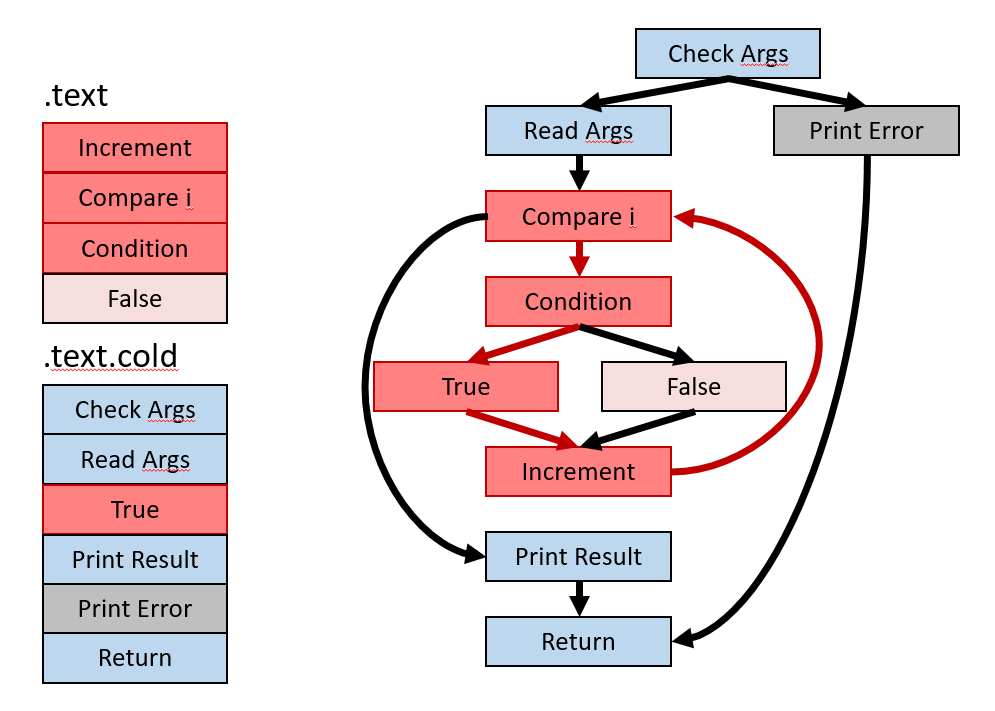
\includegraphics[width=0.8\linewidth]{_4}
    }
    \caption{Граф потока управления с измененным профилем}\label{fig:CFGProfile2}
\end{figure}

Для решения данной проблемы необходимо покрыть все возможные сценарии работы данного приложения. В итоге получив запуски с горячими линейными участками как «True», так и «False», суммарная профильная информация позволит BOLT расположить обе ветки исполнения в оптимизированной секции вместе (рисунок \cref{fig:CFGProfile3})\cite{Lin2021}.
 
\begin{figure}[!h]
    \centerfloat{
        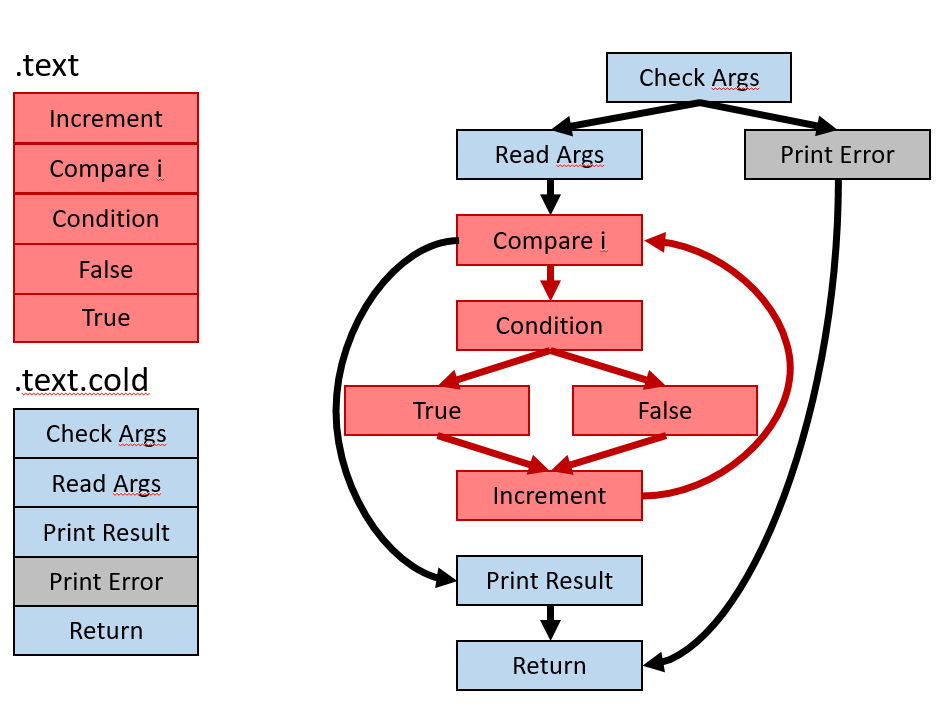
\includegraphics[width=0.8\linewidth]{_5}
    }
    \caption{Граф потока управления с суммарным профилем}\label{fig:CFGProfile3}
\end{figure}
Теперь выделенными в горячую секцию оказываются два сценария. Если при запуске используется только один сценарий, то второй будет занимать место в оптимизированной секции. Учитывая расположение в новой секции линейных участков, предпочтительнее использовать «False» ветку, так как она лежит непосредственно после участка «Condition». В случае с веткой «True» будет происходить захват линейного участка «False».

Для того чтобы этого не происходило, необходимо произвести копирование горячих линейных участков, которые относятся к различным сценариям: линейные участки «Increment» «Compare i» «Condition». Таким образом, будут созданы их копии сценария «True»: «Increment*» «Compare i*» «Condition*» (рисунок \cref{fig:CFGProfile4}).
 
\begin{figure}[!h]
    \centerfloat{
        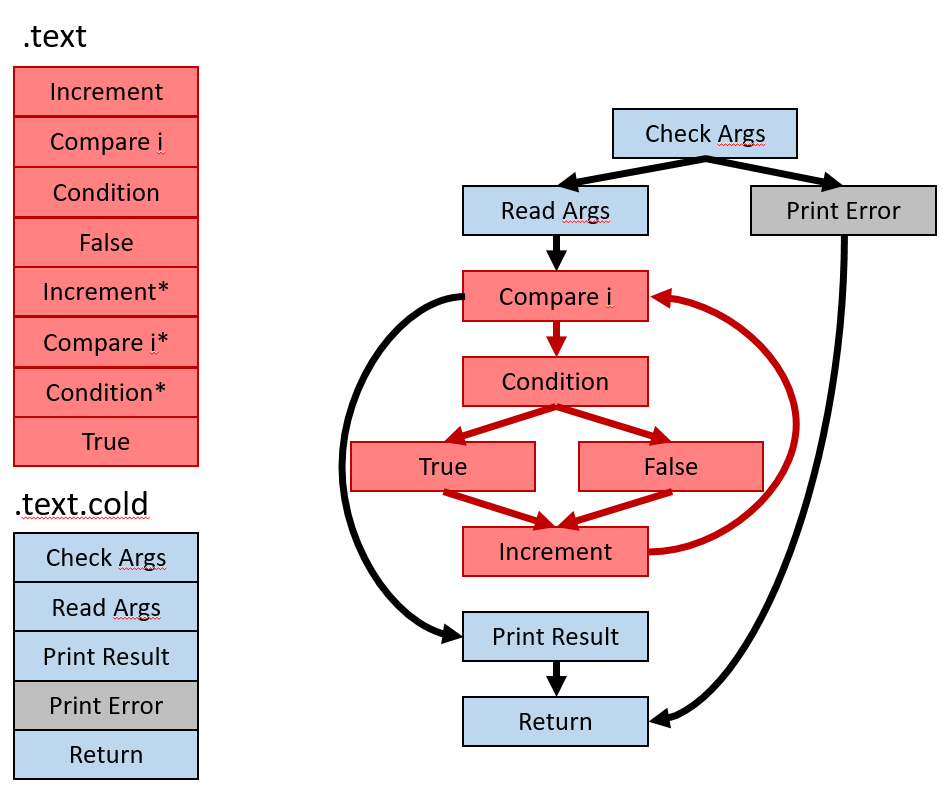
\includegraphics[width=0.8\linewidth]{_6}
    }
    \caption{Оптимизированная секция с дублированием кода}\label{fig:CFGProfile4}
\end{figure}
После всех преобразований полученная оптимизированная секция будет содержать в себе два непересекающихся сценария.

Рассмотрим, как будет происходить выбор исполняемого сценария (рисунок \cref{fig:CFGSec1}). После запуска приложения, проверки и считывания аргументов исполнение переходит в линейный участок «Compare i» произвольного сценария (для определенности «False»). После этого в линейном участке «Condition» будет происходить выбор нужной ветки исполнения. Это приведет к выбору сценария, по которому пойдёт дальнейшее исполнение.

 
\begin{figure}[!h]
    \centerfloat{
        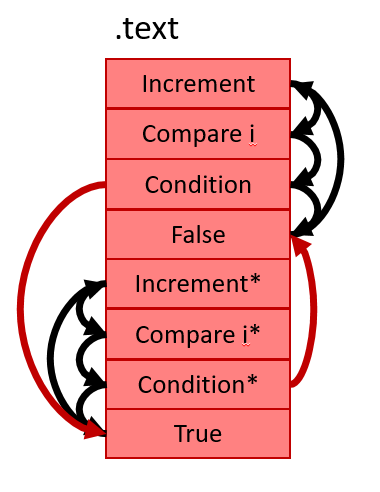
\includegraphics[width=0.5\linewidth]{_7}
    }
    \caption{Поток управления по секции с дублированием кода}\label{fig:CFGSec1}
\end{figure}
На рисунке красными стрелками отображены переходы между сценариями. Из-за дублирования кода размер секции стал больше, но таким образом удалось изолировать сценарии друг от друга. Однако, если будут частые переключения между ними, то в итоге количество постоянно исполняемого кода будет включать себя и оригинальные линейные участки, и их дубликаты. Самый сложный случай – чередование сценариев «True» и «False». В этом случае последовательность исполнения будет следующая:
«Condition» => «True» => «Increment*» => «Compare i*» => «Condition*» => «False» => «Increment» => «Compare i» => «Condition» => «True» => …
В итоге получается 4 варианта реализации оптимизированной секции (рисунок \cref{fig:CFGSec2}).
 
\begin{figure}[!h]
    \centerfloat{
        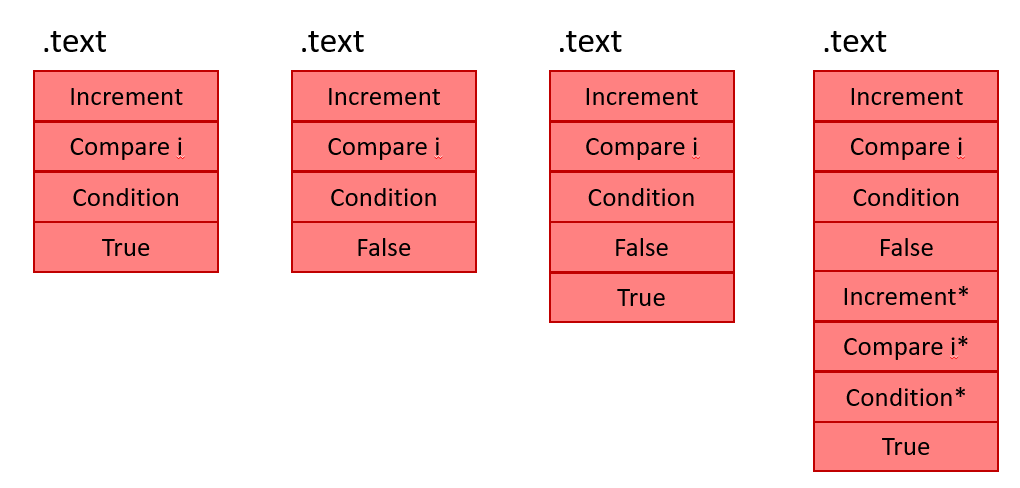
\includegraphics[width=1.0\linewidth]{_8}
    }
    \caption{Варианты оптимизированных секций}\label{fig:CFGSec2}
\end{figure}
Первые два варианта подходят только в том случае, если есть уверенность в отсутствии запусков сценариев, не помещенных в секцию. При наличии исполнения обоих сценариев и частом переключении между ними необходимо использовать третий вариант секции. И если переключения между сценариями редкие, то необходимо использовать 4 вариант, вариант оптимизированной секции с дублированием общего кода.
На практике можно реализовать несколько случаев в бинарном файле и поставить специальные счетчики, которые будут перенаправлять между вариантами оптимизированных секций, но данный вариант рассматриваться не будет.

Приведенный пример содержит в себе мало исполняемого кода, поэтому дублирование кода не сильно увеличит размер секции, но если рассмотреть примеры реальных приложений, пересечение между сценариями могут покрывать больше половины секции кода. В данном варианте анализ сценариев исполнения и доказательство необходимости дублирования кода становится важной задачей для повышения производительности приложения.

Трасса исполнения содержит в себе гораздо больше информации, чем профиль, который в конечном итоге используется для оптимизации приложения. Помимо количества сделанных переходов на каждой инструкции изменения программного счетчика есть информация о последовательности сделанных переходов, которую можно учитывать во время оптимизации.

Также для оптимизации можно добавить в трассу информацию про использованные адреса в инструкциях загрузки и выгрузки. Таким образом, можно достать подробную информацию для оптимизации данных в бинарном файле.

\section{Мультипрофильный анализ трасс исполнения}\label{sec:ch4/sect3}
Для проведения анализа приложения необходимы трассы исполнения, собранные с помощью динамической бинарной инструментации\cite{Rimsa2021} и покрывающие большинство сценариев использования приложения \cite{confbib3}. В итоге необходимо получить соотношение кода с выявленными сценариями. Для операций с первой величиной будет использоваться понятие линейного участка кода (базовый блок). Для действий, связанных со сценариями, будет использоваться понятие фазы из статьи \cite{Vandeputte2007}. В итоге в ходе анализа многопрофильности необходимо построить соответствие между линейными участками и выявленными фазами \cite{Lin2016}.

Трасса разбивается на одинаковые интервалы по количеству инструкций. Это необходимо для анализа исполнения в рамках одного отрезка времени – интервала инструкций, так как требуется найти похожие интервалы и объединить их в фазы \cite{Lebras2019}.

Для большей наглядности граф исполнения отображается в виде тепловой карты. По оси X – интервалы инструкций согласно времени исполнения, по оси Y – номер линейного участка кода (рисунок \cref{fig:HeatMap1}).

\begin{figure}[!h]
    \centerfloat{
        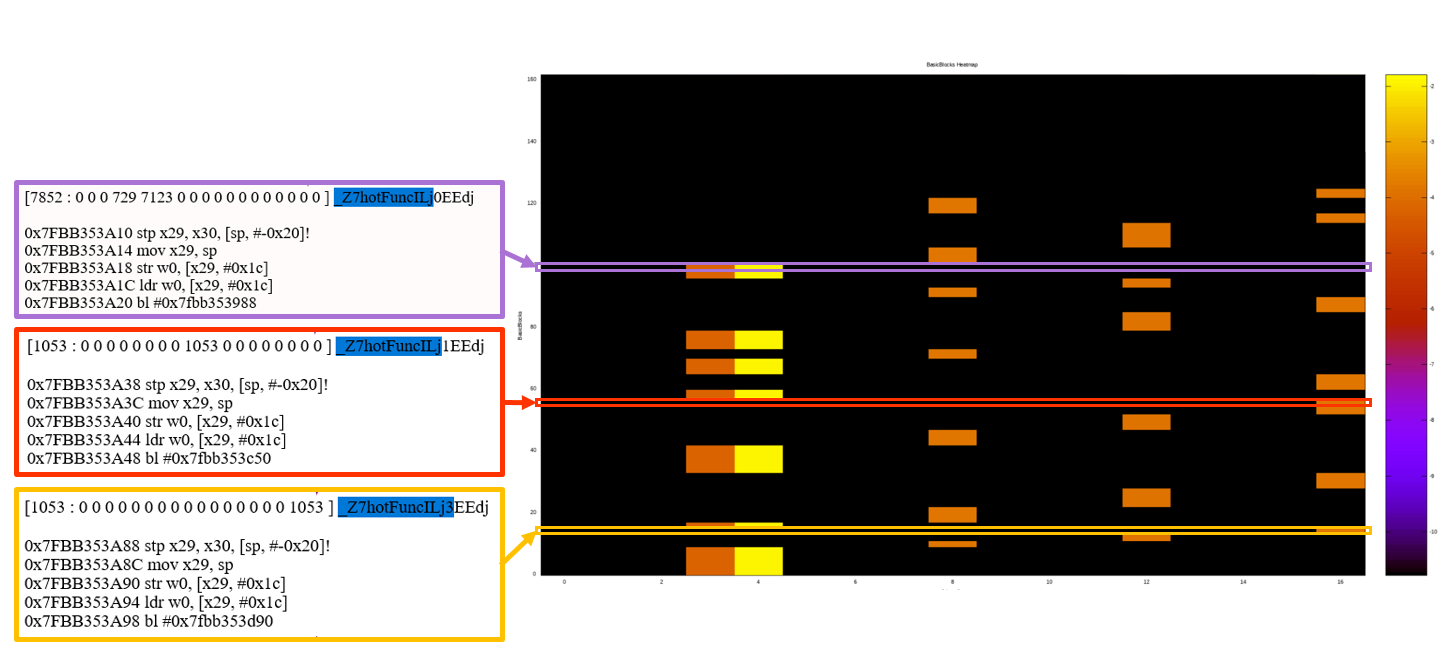
\includegraphics[width=1.0\linewidth]{_9}
    }
    \caption{Построение тепловой карты линейных участков}\label{fig:HeatMap1}
\end{figure}

На каждом интервале исполняется определенный набор линейных участков кода, который характеризует интервал инструкций. Если составить n-мерное пространство, где n – количество линейных участков кода, а координаты – количество исполненных соответствующих линейных участков на выбранном интервале, то каждому интервалу в данном пространстве будет соответствовать точка.

Необходимо произвести кластеризацию интервалов: каждый полученный кластер интервалов инструкций будет означать определенную фазу. Кластеризация будет проводиться с помощью итеративного алгоритма объединения фаз \cite{Vandeputte2007}.

В начале алгоритма каждый интервал считается отдельной фазой. Вычисляются расстояния между текущими фазами, выбирается наименьшее из полученных, и выбранная пара ближайших фаз объединяются. После чего итерация повторяется до тех пор, пока не останется необходимое количество фаз (рисунок \cref{fig:HeatMap2}). Данный алгоритм является жадной кластеризацией, параллельная версия которой была реализована в рамках проделанного исследования.
 
\begin{figure}[!h]
    \centerfloat{
        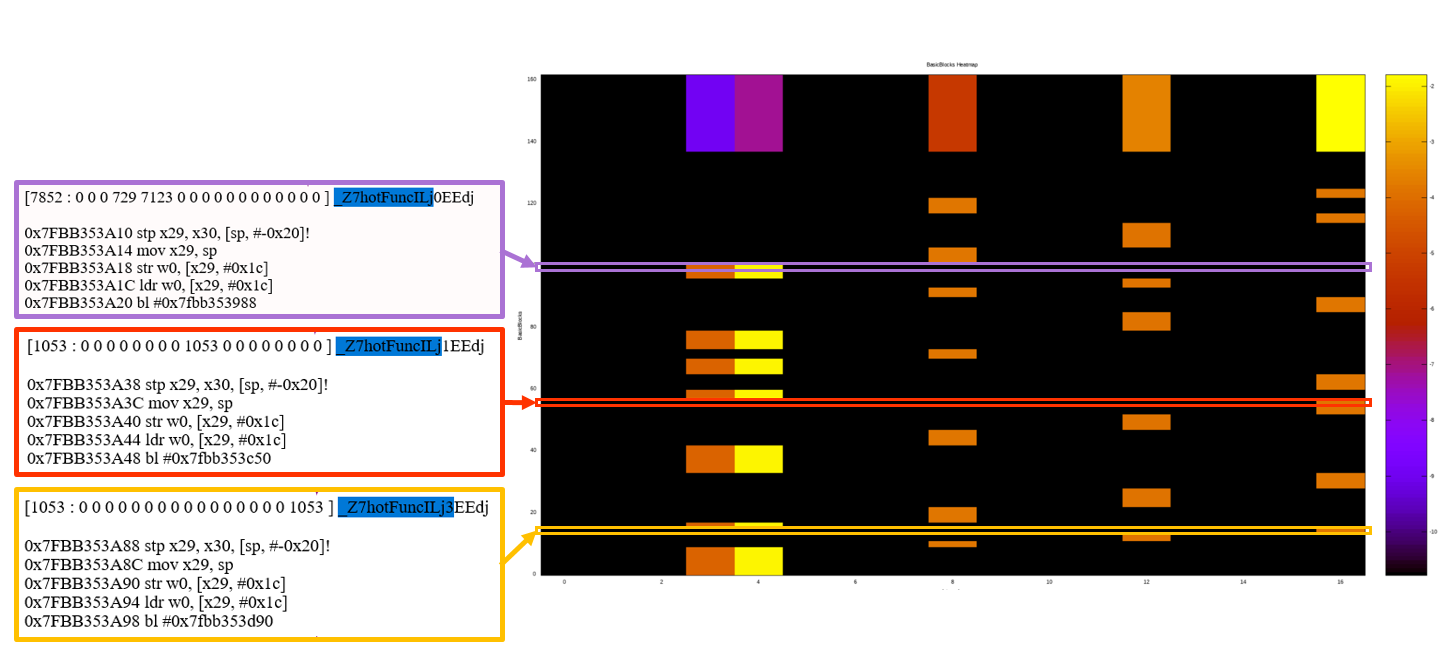
\includegraphics[width=1.0\linewidth]{_10}
    }
    \caption{Добавление фаз исполнения в тепловую карту (верхняя строка тепловой карты)}\label{fig:HeatMap2}
\end{figure}

После выделения фаз начинается стадия их анализа. Для примера анализа рассмотрим приложение с тремя режимами исполнения и без пересечения кода (рисунок \cref{fig:HeatmapEx}).

 
\begin{figure}[!h]
    \centerfloat{
        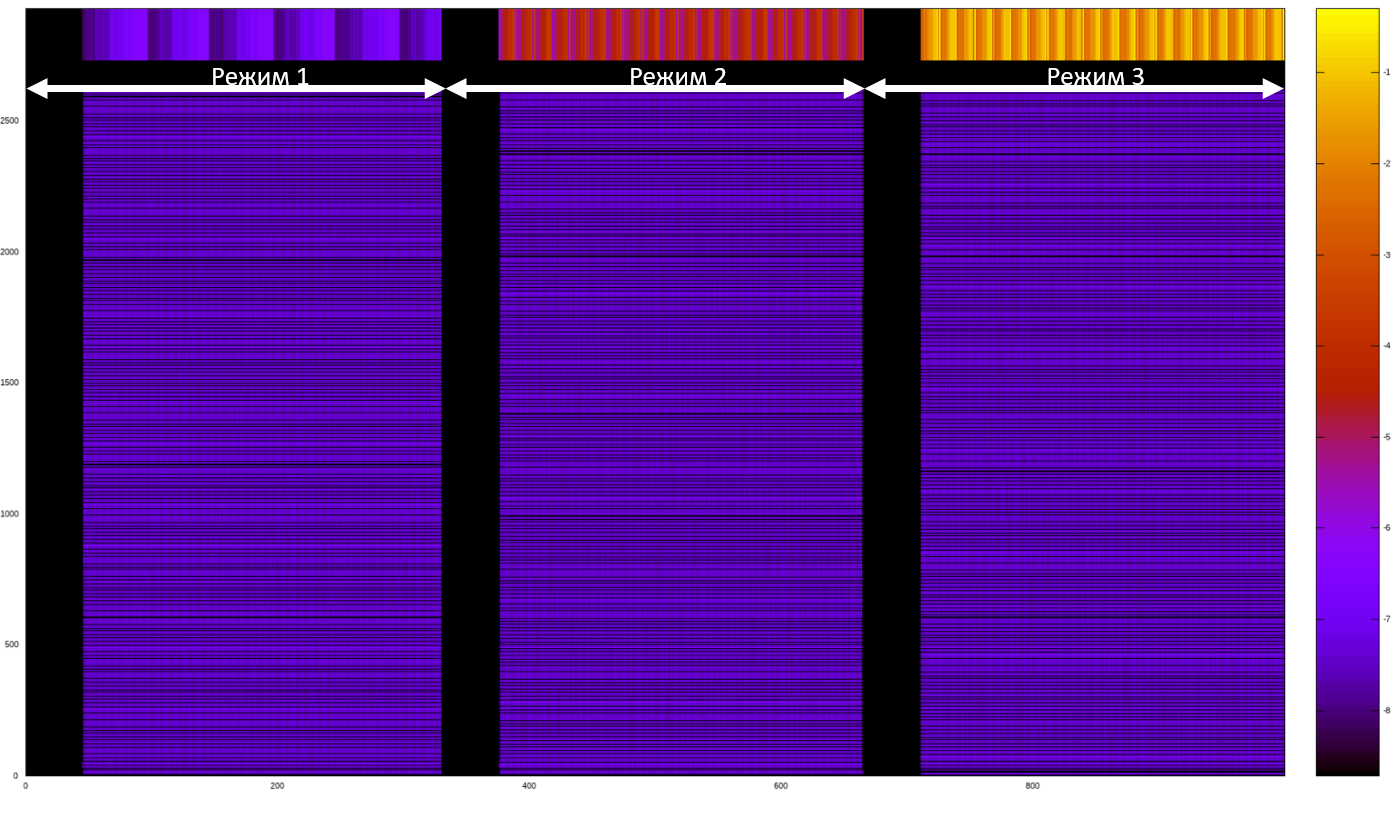
\includegraphics[width=1.0\linewidth]{_11}
    }
    \caption{Тепловая карта приложения, запущенного в трех разных режимах}\label{fig:HeatmapEx}
\end{figure}
По переключениям между фазами строится граф исполнения (рисунок \cref{fig:Phase1}). Он является аналогом графа потока управления, но на более высоком уровне, показывая переключения не между линейными участками, а между макросостояниями исполнения программы.
 

\begin{figure}[!h]
    \centerfloat{
        \includegraphics[width=1.0\linewidth]{_12}
    }
    \caption{Граф потока управления по фазам}\label{fig:Phase1}
\end{figure}
Получив граф фаз состояний можно проанализировать сценарии приложения и выделить характерные особенности, используемые затем в оптимизациях.

Если произвести сравнение фаз со сценариями исполнения приложения, то заметна корреляция: на каждый запуск приходятся свои собственные фазы без пересечения (рисунок \cref{fig:Phase2}).
 
\begin{figure}[!h]
    \centerfloat{
        \includegraphics[width=1.0\linewidth]{_13}
    }
    \caption{Соответствие графа потока управления по фазам со сценариями}\label{fig:Phase2}
\end{figure}
Однако, это синтетический пример, поэтому пересечения между сценариями исключены, что позволяет провести оптимизацию перекомпоновки кода без применения дублирования. В реальных приложениях пересечения могут встречаться, и для повышения локальности кода его части необходимо будет дублировать.

Завершение анализа приложения требует построения соответствия между фазами и линейными участками приложения. Для этого каждый линейный участок анализируется отдельно, выбирается интервал с его наибольшим количеством исполнений. Линейному участку кода будет соответствовать фаза, которая включает в себя этот интервал.

В итоге каждому линейному участку кода соответствует фаза, обозначенная на тепловой карте в столбце слева (рисунок \cref{fig:MP1}).
 
\begin{figure}[!h]
    \centerfloat{
        \includegraphics[width=1.0\linewidth]{_14}
    }
    \caption{Пример построения соответствия линейных участков фазам}\label{fig:MP1}
\end{figure}

Получив соответствие линейных участков кода и фаз (рисунок \cref{fig:MP2}), расположение в оптимизированной секции кода будет производиться при размещении всего кода в одной фазе. Для этого производится модификация профильной информации для бинарного оптимизатора BOLT, с прибавлением константы смещения между фазами. Таким образом бинарные функции одной фазы вероятнее окажутся на соседних адресах в оптимизированном бинарном файле (рисунок \cref{fig:MP3}).

Если рассмотреть синтетический тест с разделенными сценариями использованию, то после анализа и оптимизации код будет расположен в оптимизированной секции таким образом, что регионы исполнения сценариев не будут пересекаться.

\begin{figure}[!h]
    \centerfloat{
        \includegraphics[width=1.0\linewidth]{_15а}
    }
    \caption{Пример тепловой карты приложения до сортировки}\label{fig:MP2}
\end{figure}

\begin{figure}[!h]
    \centerfloat{
        \includegraphics[width=1.0\linewidth]{_15б}
    }
    \caption{Пример тепловой карты приложения после сортировки}\label{fig:MP3}
\end{figure}

Без проведения мультипрофильного анализа бинарный оптимизатор BOLT имеет профильную информацию, по которой можно получить подобный результат. На более сложных примерах восстановление глобального потока управления становится неподъемной для BOLTа задачей.

При использовании данного анализа на реальном приложении визуально видно различия в режимах исполнения (рисунок \cref{fig:MP4}). Данные различия позволяют провести отдельный класс приложений, основанный на пересечениях фаз.

\begin{figure}[!h]
    \centerfloat{
        \includegraphics[width=1.0\linewidth]{fortnite}
    }
    \caption{Пример тепловой карты для реальной библиотеки приложения}\label{fig:MP4}
\end{figure}

\section{Дублирование кода на основе мультипрофиля}\label{sec:ch4/sect3}
Выстраивая соответствие между линейными участками кода и фазами, выбиралась фаза, которой принадлежит интервал инструкций с наибольшим количеством исполнений данного линейного участка. Однако, может сложиться ситуация, когда линейный участок одинаково часто исполнялся на интервалах инструкций из разных фаз. В этом случае необходимо запоминать такие линейные участки для последующего анализа необходимости дублирования данного кода \cite{Desmond2009}.

Используя эвристически подобранные соотношения, выбираются те линейные участки, которые относятся одновременно к нескольким фазам. После этого данные участки помечаются для дублирования бинарным оптимизатором BOLT (рисунок \cref{fig:MPOpt}).

\begin{figure}[!h]
    \begin{minipage}[b][][b]{0.49\linewidth}\centering
        \includegraphics[width=1.0\linewidth]{mi1} \\ а)до оптимизации
    \end{minipage}
    \hfill
    \begin{minipage}[b][][b]{0.49\linewidth}\centering
        \includegraphics[width=1.0\linewidth]{mi2} \\ б)после оптимизации
    \end{minipage}
    \caption{Дублирование кода на основе мультипрофиля}
    \label{fig:MPOpt}
\end{figure}

\section{Результаты тестирования оптимизации дублирования}\label{sec:ch4/sect3}
Для проверки анализа был использован набор тестов GeekBench (рисунок \cref{fig:GKBMP}). Были записаны трассы его исполнения на различных задачах. На тепловой карте выделены запуски различных задач, представляющие в данном случае сценарии запуска приложения. По верхней строке тепловой карты видно корректное выделение фаз на каждый отдельный тест из набора.

\begin{figure}[!h]
    \centerfloat{
        \includegraphics[width=1.0\linewidth]{_16}
    }
    \caption{Тепловая карта набора тестов Geekbench с выделенными тестами}\label{fig:GKBMP}
\end{figure}

После проведенного анализа и модификации профильной информации производится оптимизация с помощью бинарного оптимизатора BOLT (рисунок \cref{fig:CmpPerfGKB}). По результатам запуска удалось получить прирост производительности до 4\% для некоторых отдельных тестов из набора. При этом прирост на всех тестах не превышает 1\%, это связано с отсутствием больших пересечений в коде набора тестов \cite{vakbib2}.
 
\begin{figure}[!h]
    \centerfloat{
        \includegraphics[width=1.0\linewidth]{_18}
    }
    \caption{Сравнение прироста производительности}\label{fig:CmpPerfGKB}
\end{figure}

При использовании оптимизации дублирования кода на основе мультипрофильной информации получаются результаты, приведенные на рисунке \cref{fig:MPResGKB}.


\begin{figure}[!h]
    \centerfloat{
        \includegraphics[width=1.0\linewidth]{scores}
    }
    \caption{Результаты тестирования мультипрофильного дублирования кода}\label{fig:MPResGKB}
\end{figure}

\section{Вывод по главе}\label{sec:ch4/sect3}
В четвертой главе были рассмотрены дополнительные оптимизации, которые можно реализовать, используя информацию из трасс исполнения. В результате проделанной работы исследованы алгоритмы мультипрофильного анализа и написан анализатор приложений на основе трасс исполнения. Разработана визуализация тепловой карты линейных участков. Анализ с оптимизацией проверены на синтетических тестах и на тестовом наборе Geekbench.


\clearpage
           % Глава 4
\chapter*{Заключение}                       % Заголовок
\addcontentsline{toc}{chapter}{Заключение}  % Добавляем его в оглавление

%% Согласно ГОСТ Р 7.0.11-2011:
%% 5.3.3 В заключении диссертации излагают итоги выполненного исследования, рекомендации, перспективы дальнейшей разработки темы.
%% 9.2.3 В заключении автореферата диссертации излагают итоги данного исследования, рекомендации и перспективы дальнейшей разработки темы.
%% Поэтому имеет смысл сделать эту часть общей и загрузить из одного файла в автореферат и в диссертацию:

Оптимизация приложений является сложной научно-технической задачей. При этом постоянное улучшение аппаратного обеспечения 
В диссертационной работе были рассмотрены существующие технологии бинарной трансляции и, в частности, бинарной оптимизации. Главным направлением исследования являлось улучшение бинарной оптимизации под ARM архитектуру.
Основные результаты работы заключаются в следующем:
%% Согласно ГОСТ Р 7.0.11-2011:
%% 5.3.3 В заключении диссертации излагают итоги выполненного исследования, рекомендации, перспективы дальнейшей разработки темы.
%% 9.2.3 В заключении автореферата диссертации излагают итоги данного исследования, рекомендации и перспективы дальнейшей разработки темы.
\begin{enumerate}
  \item В диссертации был реализован новый алгоритм получения профильной информации формата BOLT на основе трасс исполнения приложения. В работе показано, что для определенных классов устройств это единственный способ получения полноценного профиля приложения.
  \item Было разработано ПО, транслирующее трассу исполнения приложения для архитектуры ARM в профильную информацию.
  \item Была реализована полноценная поддержка бинарного оптимизатора BOLT для ARM архитектуры, необходимая для проведения тестовых замеров на целевых приложениях. Исходная версия BOLT изначально не поддерживала оптимизацию нужных приложений.
  \item Был получен прирост производительности на 10\% при использовании бинарного оптимизатора BOLT для  целевых приложений на ARM архитектуре.
  \item Был разработан специальный универсальный формат, описывающий преобразования исполняемого файла в оптимизированный.
  \item Был разработан статический анализатор, верифицирующий оптимизированный исполняемый файл на основе оригинального файла и файла преобразования.
  \item Был создан алгоритм мультипрофильного анализа, выделяющий профили приложения на основе трасс исполнения. На его основе реализована оптимизация копирования кода.
\end{enumerate}
%% Для Диссертации поставить

      % Заключение
\nocite{Panchenko2021}
\nocite{Panchenko2019}
\nocite{Li2019}
\nocite{Moreira2021}
\nocite{Licker2020}
\nocite{Gadioli2018}
\nocite{Newell2020}
\nocite{Hazelwood2006}
\nocite{Ball1993}
\nocite{Blem2013}
\nocite{Rimsa2019}
\nocite{Desmet2005}
\nocite{Ashouri2018}
\nocite{Khan2021}
\nocite{Bruening2004}
\nocite{Neves2021}
\nocite{ODea2020}
\nocite{Savage2020}
\nocite{Fisher1992}
\nocite{Al-Tashi2019}
\nocite{Valiante2021}
\nocite{Pereira2019}
\nocite{Rimsa2021}
\nocite{Nethercote2007}
\nocite{Smith1981}
\nocite{Ottoni2021}
\nocite{Ottoni2017}
\nocite{Sari2021}
\nocite{Hong2019}
\nocite{Li2010}
\nocite{Fu2018}
\nocite{Wu1994}
\nocite{Luk2004}
\nocite{Desmond2009}
\nocite{Arif2021}
\nocite{Ottoni2018}
\nocite{Ajorpaz2018}
\nocite{Lavaee2019}
\nocite{Zhou2019}
\nocite{Zhou2021}
\nocite{Lattner2004}
\nocite{Holzle1994}
\nocite{Li2007}
\nocite{Bruening2003}
\nocite{Lin2016}
\nocite{Vandeputte2007}
\nocite{Lebras2019}
\nocite{Ying2020}
\nocite{Nethercote2003}
\nocite{Ovasapyan2020}
\nocite{Chen2016}
\nocite{Lin2021}
\nocite{Khan2020}
\nocite{Kalla2017}

\clearpage                                  % В том числе гарантирует, что список литературы в оглавлении будет с правильным номером страницы
%\hypersetup{ urlcolor=black }               % Ссылки делаем чёрными
%\providecommand*{\BibDash}{}                % В стилях ugost2008 отключаем использование тире как разделителя
\urlstyle{rm}                               % ссылки URL обычным шрифтом
\ifdefmacro{\microtypesetup}{\microtypesetup{protrusion=false}}{} % не рекомендуется применять пакет микротипографики к автоматически генерируемому списку литературы
\insertbibliofull                           % Подключаем Bib-базы: все статьи единым списком
% Режим с подсписками
%\insertbiblioexternal                      % Подключаем Bib-базы: статьи, не являющиеся статьями автора по теме диссертации
% Для вывода выберите и расскомментируйте одно из двух
%\insertbiblioauthor                        % Подключаем Bib-базы: работы автора единым списком 
%\insertbiblioauthorgrouped                 % Подключаем Bib-базы: работы автора сгруппированные (ВАК, WoS, Scopus и т.д.)
\ifdefmacro{\microtypesetup}{\microtypesetup{protrusion=true}}{}
\urlstyle{tt}                               % возвращаем установки шрифта ссылок URL
%\hypersetup{ urlcolor={urlcolor} }          % Восстанавливаем цвет ссылок      % Список литературы
\include{Dissertation/lists}           % Список изображений (иллюстративный материал)

\setcounter{totalchapter}{\value{chapter}} % Подсчёт количества глав

%%% Настройки для приложений
\appendix
% Оформление заголовков приложений ближе к ГОСТ:
\setlength{\midchapskip}{20pt}
\renewcommand*{\afterchapternum}{\par\nobreak\vskip \midchapskip}
\renewcommand\thechapter{\Asbuk{chapter}} % Чтобы приложения русскими буквами нумеровались

\chapter{Программный код основных синтетических тестов}\label{app:A}

В данном приложении приводится исходный код трёх основных синтетических тестов, которые использовались для проверки бинарного оптимизатора BOLT. Основным методом получения большого размера бинарного файла (> 10 МБ) было использование рекурсивных шаблонов. С их помощью компилятор создавал множественные копии функций с разными шаблонными константами, тем самым увеличивая размер кода до нужного значения.

\begingroup
\captiondelim{ } % разделитель идентификатора с номером от наименования
\lstinputlisting[lastline=140,language={[ISO]C++},caption={Синтетический тест без стандартной библиотеки},label={lst:external1}]{listings/start.cpp}
\endgroup

\begingroup
\captiondelim{ } % разделитель идентификатора с номером от наименования
\lstinputlisting[lastline=78,language={[x86masm]Assembler},caption={Стартовый ассемблерный код для ARM архитектуры для теста без стандартной библиотеки},label={lst:external1}]{listings/start_ARM.S}
\endgroup

\begingroup
\captiondelim{ } % разделитель идентификатора с номером от наименования
\lstinputlisting[lastline=78,language={[x86masm]Assembler},caption={Стартовый ассемблерный код для x86 архитектуры для теста без стандартной библиотеки},label={lst:external1}]{listings/start_x86.S}
\endgroup

\begingroup
\captiondelim{ } % разделитель идентификатора с номером от наименования
\lstinputlisting[lastline=160,language={[ISO]C++},caption={Синтетический тест с использованием стандартной библиотеки},label={lst:external1}]{listings/1k.cpp}
\endgroup

\begingroup
\captiondelim{ } % разделитель идентификатора с номером от наименования
\lstinputlisting[lastline=192,language={[ISO]C++},caption={Синтетический тест с использованием исключений и виртуальных функций},label={lst:external1}]{listings/except+virt.cpp}
\endgroup

\chapter{Ассемблерный код демонстрационного примера}\label{app:B}
В данном приложении приводится ассемблерный код демонстрационного примера, на котором были получены профиль на x86 и ARM архитектурах.

\begingroup
\captiondelim{ } % разделитель идентификатора с номером от наименования
\lstinputlisting[lastline=264,language={[x86masm]Assembler},caption={Ассемблерный код демонстрационного примера для ARM архитектуры},label={lst:ARMobj}]{listings/ARMobjdump.s}
\label{lst:ARM}
\endgroup

\begingroup
\captiondelim{ } % разделитель идентификатора с номером от наименования
\lstinputlisting[lastline=221,language={[x86masm]Assembler},caption={Ассемблерный код демонстрационного примера для x86 архитектуры},label={lst:x86obj}]{listings/x86objdump.s}
\label{lst:X86}
\endgroup


\chapter{Акты о внедрении}\label{app:С}

    \centerfloat{
        \includegraphics[width=1.0\linewidth]{Act_teach}
    }

    \centerfloat{
        \includegraphics[width=1.0\linewidth]{Act_company}
    }        % Приложения

\setcounter{totalappendix}{\value{chapter}} % Подсчёт количества приложений

\end{document}
